% LaTeX source for ``Think Stats:
% Probability and Statistics for Programmers''
% Copyright 2011  Allen B. Downey.

% License: Creative Commons Attribution-NonCommercial 3.0 Unported License.
% http://creativecommons.org/licenses/by-nc/3.0/
%

%\documentclass[10pt,b5paper]{book}
\documentclass[12pt]{book}
\usepackage[width=5.5in,height=8.5in,
  hmarginratio=3:2,vmarginratio=1:1]{geometry}

% for some of these packages, you might have to install
% texlive-latex-extra (in Ubuntu)

\usepackage[T1]{fontenc}
\usepackage{textcomp}
\usepackage{mathpazo}

%\usepackage{pslatex}

\usepackage{url}
\usepackage{fancyhdr}
\usepackage{graphicx}
\usepackage{subfig}
\usepackage{amsmath}
\usepackage{amsthm}
%\usepackage{amssymb}
\usepackage{makeidx}
\usepackage{setspace}
\usepackage{hevea}                           
\usepackage{upquote}

\title{Think Stats}
\author{Allen B. Downey}

\newcommand{\thetitle}{Think Stats: Probability and Statistics for Programmers}
\newcommand{\theversion}{1.5.7}

% these styles get translated in CSS for the HTML version
\newstyle{a:link}{color:black;}
\newstyle{p+p}{margin-top:1em;margin-bottom:1em}
\newstyle{img}{border:0px}

% change the arrows in the HTML version
\setlinkstext
  {\imgsrc[ALT="Previous"]{back.png}}
  {\imgsrc[ALT="Up"]{up.png}}
  {\imgsrc[ALT="Next"]{next.png}} 

\makeindex

\newif\ifplastex
\plastexfalse

\begin{document}

\frontmatter

\ifplastex
    \newcommand{\dd}{\mathit{d}}
    \newcommand{\e}{\mathit{e}}
    \newcommand{\f}{\mathit{f}}
    \newcommand{\gee}{\mathit{g}}
    \newcommand{\ii}{\mathit{i}}
    \newcommand{\kk}{\mathit{k}}
    \newcommand{\n}{\mathit{n}}
    \newcommand{\m}{\mathit{m}}
    \newcommand{\w}{\mathit{w}}
    \newcommand{\p}{\mathit{p}}
    \newcommand{\s}{\mathit{s}}
    \newcommand{\x}{\mathit{x}}
    \newcommand{\X}{\mathit{X}}
    \newcommand{\y}{\mathit{y}}
    \newcommand{\Y}{\mathit{Y}}
    \newcommand{\z}{\mathit{z}}
    \newcommand{\Z}{\mathit{Z}}
    \newcommand{\E}{\mathit{E}}
    \newcommand{\OO}{\mathit{O}}
    \newcommand{\HH}{\mathit{H}}
    \newcommand{\A}{\mathit{A}}
    \newcommand{\B}{\mathit{B}}
    \newcommand{\D}{\mathit{D}}
    \newcommand{\N}{\mathit{N}}
    \newcommand{\R}{\mathit{R}}
    \newcommand{\Ssq}{$S^2$}
    \newcommand{\Snsq}{$S_{n-1}^2$}
    \newcommand{\mya}{\mathit{a}}
    \newcommand{\myb}{\mathit{b}}
    \newcommand{\Prob}{\mathit{P}}
    \newcommand{\xsubi}{\mathit{x}\sub{i}}
    \newcommand{\psubi}{\mathit{p}\sub{i}}
    \newcommand{\mymu}{\mathit{\mu}}
    \newcommand{\mychi}{\mathit{\chi}}
    \newcommand{\myalpha}{\mathit{\alpha}}
    \newcommand{\mysigma}{\mathit{\sigma}}
    \newcommand{\myrho}{\mathit{\rho}}
    \newcommand{\mylambda}{\mathit{\lambda}}
    \newcommand{\mydelta}{\mathit{\delta}}
    \newcommand{\sigmasq}{\mathit{\sigma}\super{2}}

    \newcommand{\plus}{+}
    \newcommand{\mytimes}{\times}
    \newcommand{\mydivide}{/}
    \newcommand{\mystar}{\lowast}
    \newcommand{\mysim}{\sim}
    \newcommand{\myapprox}{\approx}
    \newcommand{\mynormal}{$\mathcal{N}$}

    \newcommand{\myslope}{\mathit{\beta}}
    \newcommand{\myinter}{\mathit{\alpha}}

    \newcommand{\myeps}{\mathit{\varepsilon}}
    \newcommand{\myxbar}{\uxbar}
    \newcommand{\myybar}{\uybar}
    \newcommand{\mynhat}{$\nhat$}
    \newcommand{\myle}{\ule}
\else
    \newcommand{\dd}{$d$}
    \newcommand{\e}{$e$}
    \newcommand{\f}{$f$}
    \newcommand{\gee}{$g$}
    \newcommand{\ii}{$i$}
    \newcommand{\kk}{$k$}
    \newcommand{\n}{$n$}
    \newcommand{\m}{$m$}
    \newcommand{\w}{$w$}
    \newcommand{\p}{$p$}
    \newcommand{\s}{$s$}
    \newcommand{\x}{$x$}
    \newcommand{\X}{$X$}
    \newcommand{\y}{$y$}
    \newcommand{\Y}{$Y$}
    \newcommand{\z}{$z$}
    \newcommand{\Z}{$Z$}
    \newcommand{\E}{$E$}
    \newcommand{\OO}{$O$}
    \newcommand{\HH}{$H$}
    \newcommand{\A}{$A$}
    \newcommand{\B}{$B$}
    \newcommand{\D}{$D$}
    \newcommand{\N}{$N$}
    \newcommand{\R}{$R$}
    \newcommand{\Ssq}{$S^2$}
    \newcommand{\Snsq}{$S_{n-1}^2$}
    \newcommand{\mya}{$a$}
    \newcommand{\myb}{$b$}
    \newcommand{\Prob}{$P$}
    \newcommand{\xsubi}{$x_i$}
    \newcommand{\psubi}{$p_i$}
    \newcommand{\mymu}{$\mu$}
    \newcommand{\mychi}{$\chi$}
    \newcommand{\myalpha}{$\alpha$}
    \newcommand{\mysigma}{$\sigma$}
    \newcommand{\myrho}{$\rho$}
    \newcommand{\mylambda}{$\lambda$}
    \newcommand{\mydelta}{$\delta$}
    \newcommand{\sigmasq}{$\sigma^2$}

    \newcommand{\plus}{$+$}
    \newcommand{\minus}{$-$}
    \newcommand{\mytimes}{$\times$}
    \newcommand{\mydivide}{$/$}

    \newcommand{\sub}[1]{$_{#1}$}
    \newcommand{\super}[1]{$^{#1}$}
    \newcommand{\mystar}{$\star$}
    \newcommand{\mysim}{$\sim$}
    \newcommand{\myapprox}{$\approx$}
    \newcommand{\normal}{\mathcal{N}}
    \newcommand{\mynormal}{$\mathcal{N}$}

    \newcommand{\myslope}{$\beta$}
    \newcommand{\myinter}{$\alpha$}

    \newcommand{\myeps}{$\varepsilon$}

    \newcommand{\myxbar}{$\xbar$}
    \newcommand{\myybar}{$\ybar$}
    \newcommand{\mynhat}{$\nhat$}
    \newcommand{\myle}{$\le$}
    \newcommand{\Eqn}[1]{\quad #1}
\fi

\newcommand{\Erdos}{Erd\H{o}s}
\newcommand{\nhat}{\hat{N}}
\newcommand{\eps}{\varepsilon}
\newcommand{\slope}{\beta}
\newcommand{\inter}{\alpha}
\newcommand{\xbar}{\bar{x}}
\newcommand{\ybar}{\bar{y}}
\newcommand{\PMF}{\mathrm{PMF}}
\newcommand{\PDF}{\mathrm{PDF}}
\newcommand{\CDF}{\mathrm{CDF}}
\newcommand{\ICDF}{\mathrm{ICDF}}

\ifplastex
    \usepackage{localdef}
    \maketitle

\newcount\anchorcnt
\newcommand*{\Anchor}[1]{%
  \@bsphack%
    \Hy@GlobalStepCount\anchorcnt%
    \edef\@currentHref{anchor.\the\anchorcnt}% 
    \Hy@raisedlink{\hyper@anchorstart{\@currentHref}\hyper@anchorend}% 
    \M@gettitle{}\label{#1}% 
    \@esphack%
}


\else

%%% EXERCISE

\newtheoremstyle{exercise}% name of the style to be used
  {\topsep}% measure of space to leave above the theorem. E.g.: 3pt
  {\topsep}% measure of space to leave below the theorem. E.g.: 3pt
  {}% name of font to use in the body of the theorem
  {0pt}% measure of space to indent
  {\bfseries}% name of head font
  {}% punctuation between head and body
  { }% space after theorem head; " " = normal interword space
  {}% Manually specify head

\theoremstyle{exercise}
\newtheorem{exercise}{Exercise}[chapter]

%\newcounter{exercise}[chapter]
%\newcommand{\nextexercise}{\refstepcounter{exercise}}

%\newenvironment{exercise}{\nextexercise \noindent \textbf{Exercise \thechapter.\theexercise} \begin{itshape} \noindent}{\end{itshape}}

\input{latexonly}

\begin{latexonly}

\renewcommand{\blankpage}{\thispagestyle{empty} \quad \newpage}

%\blankpage
%\blankpage

% TITLE PAGES FOR LATEX VERSION

%-half title--------------------------------------------------
\thispagestyle{empty}

\begin{flushright}
\vspace*{2.0in}

\begin{spacing}{3}
{\huge Think Stats: Probability and Statistics for Programmers}\\
{\Large }
\end{spacing}

\vspace{0.25in}

Version \theversion

\vfill

\end{flushright}

%--verso------------------------------------------------------

\blankpage
\blankpage
%\clearemptydoublepage
%\pagebreak
%\thispagestyle{empty}
%\vspace*{6in}

%--title page--------------------------------------------------
\pagebreak
\thispagestyle{empty}

\begin{flushright}
\vspace*{2.0in}

\begin{spacing}{3}
{\huge Think Stats}\\
{\Large Probability and Statistics for Programmers}
\end{spacing}

\vspace{0.25in}

Version \theversion

\vspace{1in}


{\Large
Allen B. Downey\\
}


\vspace{0.5in}

{\Large Green Tea Press}

{\small Needham, Massachusetts}

%\includegraphics[width=1in]{figs/logo1.eps}
\vfill

\end{flushright}


%--copyright--------------------------------------------------
\pagebreak
\thispagestyle{empty}

{\small
Copyright \copyright ~2011 Allen B. Downey.


\vspace{0.2in}

\begin{flushleft}
Green Tea Press       \\
9 Washburn Ave \\
Needham MA 02492
\end{flushleft}

Permission is granted to copy, distribute, and/or modify this document
under the terms of the Creative Commons Attribution-NonCommercial 3.0 Unported
License, which is available at \url{http://creativecommons.org/licenses/by-nc/3.0/}.

The original form of this book is \LaTeX\ source code.  Compiling this
code has the effect of generating a device-independent representation
of a textbook, which can be converted to other formats and printed.

The \LaTeX\ source for this book is available from
\url{http://thinkstats.com}.

The cover for this book is based on a photo by Paul Friel
(\url{http://flickr.com/people/frielp/}), who made it available under
the Creative Commons Attribution license.  The original photo
is at \url{http://flickr.com/photos/frielp/11999738/}.

\vspace{0.2in}

} % end small

\end{latexonly}


% HTMLONLY

\begin{htmlonly}

% TITLE PAGE FOR HTML VERSION

{\Large \thetitle}

{\large Allen B. Downey}

Version \theversion

\vspace{0.25in}

Copyright 2011 Allen B. Downey

\vspace{0.25in}

Permission is granted to copy, distribute, and/or modify this document
under the terms of the Creative Commons Attribution-NonCommercial 3.0
Unported License, which is available at
\url{http://creativecommons.org/licenses/by-nc/3.0/}.

\setcounter{chapter}{-1}

\end{htmlonly}

\fi
% END OF THE PART WE SKIP FOR PLASTEX

\chapter{Preface}
\label{preface}

\section*{Why I wrote this book}

{\em Think Stats: Probability and Statistics for Programmers} is a
textbook for a new kind of introductory prob-stat class.  
It emphasizes the use of statistics to explore large datasets.  It
takes a computational approach, which has several advantages:

\begin{itemize}

\item Students write programs as a way of developing and testing their
  understanding.  For example, they write functions to compute a least
  squares fit, residuals, and the coefficient of determination.
  Writing and testing this code requires them to understand the
  concepts and implicitly corrects misunderstandings.

\item Students run experiments to test statistical behavior.  For
  example, they explore the Central Limit Theorem (CLT) by generating
  samples from several distributions.  When they see that the sum of
  values from a Pareto distribution doesn't converge to normal, they
  remember the assumptions the CLT is based on.

\item Some ideas that are hard to grasp mathematically are easy to
  understand by simulation.  For example, we approximate p-values by
  running Monte Carlo simulations, which reinforces the meaning of the
  p-value.

\item Using discrete distributions and computation makes it possible
  to present topics like Bayesian estimation that are not usually
  covered in an introductory class.  For example, one exercise asks
  students to compute the posterior distribution for the ``German tank
  problem,'' which is difficult analytically but surprisingly easy
  computationally.

\item Because students work in a general-purpose programming language
  (Python), they are able to import data from almost any
  source.  They are not limited to data that has been cleaned and
  formatted for a particular statistics tool.

\end{itemize}

The book lends itself to a project-based approach.  In my class, students
work on a semester-long project that requires them to pose a statistical
question, find a dataset that can address it, and apply each of the
techniques they learn to their own data.

To demonstrate the kind of analysis I want students to do,
the book presents a case study that runs through all of the chapters.
It uses data from two sources:

\begin{itemize}

\item The National Survey of Family Growth (NSFG), conducted by the
  U.S. Centers for Disease Control and Prevention (CDC) to gather
  ``information on family life, marriage and divorce, pregnancy,
  infertility, use of contraception, and men's and women's health.''
  (See \url{http://cdc.gov/nchs/nsfg.htm}.)

\item The Behavioral Risk Factor Surveillance System (BRFSS),
  conducted by the National Center for Chronic Disease Prevention and
  Health Promotion to ``track health conditions and risk behaviors in
  the United States.''  (See \url{http://cdc.gov/BRFSS/}.)

\end{itemize}

Other examples use data from the IRS, the U.S. Census, and
the Boston Marathon.


\section*{How I wrote this book}

When people write a new textbook, they usually start by
reading a stack of old textbooks.  As a result, most books
contain the same material in pretty much the same order.  Often there
are phrases, and errors, that propagate from one book to the next;
Stephen Jay Gould pointed out an example in his essay, ``The Case of
the Creeping Fox Terrier\footnote{A breed of dog that is about half
  the size of a Hyracotherium (see
  \url{http://wikipedia.org/wiki/Hyracotherium}).}.''

I did not do that.  In fact, I used almost no printed material while I
was writing this book, for several reasons:

\begin{itemize}

\item My goal was to explore a new approach to this material, so I didn't
want much exposure to existing approaches.

\item Since I am making this book available under a free license, I wanted
to make sure that no part of it was encumbered by copyright restrictions.

\item Many readers of my books don't have access to libraries of
printed material, so I tried to make references to resources that are
freely available on the Internet.

\item Proponents of old media think that the exclusive
use of electronic resources is lazy and unreliable.  They might be right
about the first part, but I think they are wrong about the second, so
I wanted to test my theory.

% http://www.ala.org/ala/mgrps/rts/nmrt/news/footnotes/may2010/in_defense_of_wikipedia_bonnett.cfm

\end{itemize}

The resource I used more than any other is Wikipedia, the bugbear
of librarians everywhere.  In general, the articles I read on
statistical topics were very good (although I made a few small changes
along the way).  I include references to Wikipedia pages throughout
the book and I encourage you to follow those links; in many cases, the
Wikipedia page picks up where my description leaves off.  The
vocabulary and notation in this book are generally consistent with
Wikipedia, unless I had a good reason to deviate.

Other resources I found useful were Wolfram MathWorld and (of course)
Google.  I also used two books, David MacKay's {\em Information
  Theory, Inference, and Learning Algorithms}, which is the book that
got me hooked on Bayesian statistics, and Press et al.'s {\em
  Numerical Recipes in C}.  But both books are available online,
so I don't feel too bad.

Allen B. Downey \\*
Needham MA \\*

Allen B. Downey is a Professor of Computer Science at 
the Franklin W. Olin College of Engineering.




%\section*{Acknowledgements}



\section*{Contributor List}

If you have a suggestion or correction, please send email to 
{\tt downey@allendowney.com}.  If I make a change based on your
feedback, I will add you to the contributor list
(unless you ask to be omitted).
\index{contributors}

If you include at least part of the sentence the
error appears in, that makes it easy for me to search.  Page and
section numbers are fine, too, but not quite as easy to work with.
Thanks!

\small

\begin{itemize}

\item Lisa Downey and June Downey read an early draft and made many
corrections and suggestions.

\item Steven Zhang found several errors.

\item Andy Pethan and Molly Farison helped debug some of the solutions,
and Molly spotted several typos.

\item Andrew Heine found an error in my error function.

\item Dr. Nikolas Akerblom knows how big a Hyracotherium is.

\item Alex Morrow clarified one of the code examples.

\item Jonathan Street caught an error in the nick of time.

\item G\'{a}bor Lipt\'{a}k found a typo in the book and the relay race solution.

\item Many thanks to Kevin Smith and Tim Arnold for their work on
plasTeX, which I used to convert this book to DocBook.

\item George Caplan sent several suggestions for improving clarity.

\item Julian Ceipek found an error and a number of typos.

\item Stijn Debrouwere, Leo Marihart III, Jonathan Hammler, and Kent Johnson
found errors in the first print edition.

\item Dan Kearney found a typo.

% ENDCONTRIB

\end{itemize}

\normalsize

\clearemptydoublepage

% TABLE OF CONTENTS
\begin{latexonly}

\tableofcontents

\clearemptydoublepage

\end{latexonly}

% START THE BOOK
\mainmatter


\chapter{Statistical thinking for programmers}
\label{intro}

This book is about turning data into knowledge.  Data is cheap (at
least relatively); knowledge is harder to come by.

I will present three related pieces:

\begin{description}

\item[Probability] is the study of random events.  Most people have an
  intuitive understanding of degrees of probability, which is why you
  can use words like ``probably'' and ``unlikely'' without special
  training, but we will talk about how to make quantitative claims
  about those degrees.
\index{probability}

\item[Statistics] is the discipline of using data samples to support
  claims about populations.  Most statistical analysis is based on
  probability, which is why these pieces are usually presented
  together.
\index{statistics}

\item[Computation] is a tool that is well-suited to quantitative
  analysis, and computers are commonly used to process statistics.
  Also, computational experiments
  are useful for exploring concepts in probability and statistics.
\index{computation}

\end{description}

The thesis of this book is that if you know how to program, you can
use that skill to help you understand probability and statistics.
These topics are often presented from a mathematical perspective, and
that approach works well for some people.  But some important ideas
in this area are hard to work with mathematically and relatively
easy to approach computationally.

The rest of this chapter presents a case study motivated by a question
I heard when my wife and I were expecting our first child: do first
babies tend to arrive late?
\index{first babies}

\section{Do first babies arrive late?}

If you Google this question, you will find plenty of discussion.
Some people claim it's true, others say it's a myth, and some people
say it's the other way around: first babies come early.

In many of these discussions, people provide data to support their
claims.  I found many examples like these:

\begin{quote}

``My two friends that have given birth recently to their first babies,
BOTH went almost 2 weeks overdue before going into labour or being
induced.''

``My first one came 2 weeks late and now I think the second one is
going to come out two weeks early!!''

``I don't think that can be true because my sister was my mother's
first and she was early, as with many of my cousins.''

\end{quote}

Reports like these are called {\bf anecdotal evidence} because they
are based on data that is unpublished and usually personal.  In casual
conversation, there is nothing wrong with anecdotes, so I don't mean
to pick on the people I quoted.
\index{anecdotal evidence}

But we might want evidence that is more persuasive and
an answer that is more reliable.  By those standards, anecdotal
evidence usually fails, because:

\begin{description}

\item[Small number of observations:] If the gestation period is longer
  for first babies, the difference is probably small compared to the
  natural variation.  In that case, we might have to compare a large
  number of pregnancies to be sure that a difference exists.
\index{sample size}

\item[Selection bias:] People who join a discussion of this question
  might be interested because their first babies were late.  In that
  case the process of selecting data would bias the results.
\index{selection bias}
\index{bias!selection}

\item[Confirmation bias:] People who believe the claim might be more
  likely to contribute examples that confirm it.  People who doubt the
  claim are more likely to cite counterexamples.
\index{confirmation bias}
\index{bias!confirmation}

\item[Inaccuracy:] Anecdotes are often personal stories, and often
  misremembered, misrepresented, repeated
  inaccurately, etc.

\end{description}

So how can we do better?

\section{A statistical approach}

To address the limitations of anecdotes, we will use the tools
of statistics, which include:

\begin{description}

\item[Data collection:] We will use data from a large national survey
  that was designed explicitly with the goal of generating
  statistically valid inferences about the U.S. population.
\index{data collection}

\item[Descriptive statistics:] We will generate statistics that
  summarize the data concisely, and evaluate different ways to
  visualize data.
\index{descriptive statistics}

\item[Exploratory data analysis:] We will look for
  patterns, differences, and other features that address the questions
  we are interested in.  At the same time we will check for
  inconsistencies and identify limitations.
\index{exploratory data analysis}

\item[Hypothesis testing:] Where we see apparent effects, like a
  difference between two groups, we will evaluate whether the effect
  is real, or whether it might have happened by chance.
\index{hypothesis testing}

\item[Estimation:] We will use data from a sample to estimate
  characteristics of the general population.
\index{estimation}

\end{description}

By performing these steps with care to avoid pitfalls, we can
reach conclusions that are more justifiable and more likely to be
correct.


\section{The National Survey of Family Growth}
\label{nsfg}

Since 1973 the U.S. Centers for Disease Control and Prevention (CDC)
have conducted the National Survey of Family Growth (NSFG),
which is intended to gather ``information on family life, marriage and
divorce, pregnancy, infertility, use of contraception, and men's and
women's health. The survey results are used ... to plan health services and
health education programs, and to do statistical studies of families,
fertility, and health.''\footnote{See
  \url{http://cdc.gov/nchs/nsfg.htm}.}
\index{National Survey of Family Growth}
\index{NSFG}

We will use data collected by this survey to investigate whether first
babies tend to come late, and other questions.  In order to use this
data effectively, we have to understand the design of the study.

The NSFG is a {\bf cross-sectional} study, which means that it
captures a snapshot of a group at a point in time.  The most
common alternative is a {\bf longitudinal} study, which observes a
group repeatedly over a period of time.
\index{cross-sectional study}
\index{study!cross-sectional}
\index{longitudinal study}
\index{study!longitudinal}

The NSFG has been conducted seven times; each deployment is called
a {\bf cycle}.  We will be using data from Cycle 6, which was
conducted from January 2002 to March 2003.
\index{cycle}

The goal of the survey is to draw conclusions about a
{\bf population}; the target population of the NSFG is people in
the United States aged 15-44.
\index{population}

The people who participate in a survey are called {\bf respondents};
a group of respondents is called a {\bf cohort}.
In general, cross-sectional studies are meant to be {\bf
  representative}, which means that every member of the target
population has an equal chance of participating.  Of course that ideal
is hard to achieve in practice, but people who conduct surveys come as
close as they can.
\index{respondent}
\index{representative}

The NSFG is not representative; instead it is deliberately {\bf
  oversampled}.  The designers of the study recruited three
groups---Hispanics, African-Americans and teenagers---at rates higher
than their representation in the U.S. population.
The reason for oversampling is to make sure that the number of
respondents in each of these groups is large enough to draw valid
statistical inferences.
\index{oversampling}

Of course, the drawback of oversampling is that it is not as easy
to draw conclusions about the general population based on statistics
from the survey.  We will come back to this point later.

\begin{exercise}
Although the NSFG has been conducted seven times, it is not a
longitudinal study.  Read the Wikipedia pages
\url{http://wikipedia.org/wiki/Cross-sectional_study}
and
\url{http://wikipedia.org/wiki/Longitudinal_study}
to make sure you understand why not.

\end{exercise}

\begin{exercise}
In this exercise, you will download data from the NSFG; we will use
this data throughout the book.
\index{National Survey of Family Growth}
\index{NSFG}

\begin{enumerate}

\item Go to \url{http://thinkstats.com/nsfg.html}.  Read the terms of
use for this data and click ``I accept these terms'' (assuming that you do).

\item Download the files named {\tt 2002FemResp.dat.gz} and {\tt
  2002FemPreg.dat.gz}.  The first is the respondent file, which contains
  one line for each of the 7,643 female respondents.
  The second file contains one line for each pregnancy reported by a
  respondent.

\item Online documentation of the survey is at
  \url{http://nsfg.icpsr.umich.edu/cocoon/WebDocs/NSFG/public/index.htm}.
  Browse the sections in the left navigation bar to get a sense of
  what data are included.  You can also read the questionnaires
  at \url{http://cdc.gov/nchs/data/nsfg/nsfg_2002_questionnaires.htm}.

\item The web page for this book provides code to process the data
  files from the NSFG.  Download \url{http://thinkstats.com/survey.py}
  and run it in the same directory you put the data files in.  It
  should read the data files and print the number of lines in each:
\index{{\tt survey.py}}
%
\begin{verbatim}
Number of respondents 7643
Number of pregnancies 13593
\end{verbatim}

\item Browse the code to get a sense of what it does.  The next
section explains how it works.

\end{enumerate}

\end{exercise}

\section{Tables and records}

The poet-philosopher Steve Martin once said:
\index{Martin, Steve}
\index{oeuf}
\index{chapeau}
\index{French}
%
\begin{quote}
``Oeuf'' means egg, ``chapeau'' means hat.  It's like those French
  have a different word for everything.
\end{quote}
%
Like the French, database programmers speak a slightly
different language, and since we're working with a database we need
to learn some vocabulary.
\index{database}
\index{record (database)}
\index{field (database)}
\index{table (database)}

Each line in the respondents file contains information about one
respondent.  This information is called a {\bf record}.  The
variables that make up a record are called {\bf fields}.  A
collection of records is called a {\bf table}.
\index{{\tt survey.py}}

If you read {\tt survey.py} you will see class definitions for {\tt
  Record}, which is an object that represents a record, and {\tt
  Table}, which represents a table.

There are two subclasses of
{\tt Record}---{\tt Respondent} and {\tt Pregnancy}---which
contain records from the respondent and pregnancy tables.
For the time being, these classes are empty; in particular, there
is no init method to initialize their attributes.  Instead
we will use {\tt Table.MakeRecord} to convert a line of text into
a {\tt Record} object.
\index{init method}
\index{method!init}

There are also two subclasses of {\tt Table}: {\tt Respondents}
and {\tt Pregnancies}.  The init method in each class
specifies the default name of the data file and the type of
record to create.  Each {\tt Table} object has an attribute
named {\tt records}, which is a list of {\tt Record} objects.

For each {\tt Table}, the {\tt GetFields} method returns
a list of tuples that specify the fields from the record that
will be stored as attributes in each {\tt Record} object.  (You
might want to read that last sentence twice.)

For example, here is {\tt Pregnancies.GetFields}:
%
\begin{verbatim}
    def GetFields(self):
        return [
            ('caseid', 1, 12, int),
            ('prglength', 275, 276, int),
            ('outcome', 277, 277, int),
            ('birthord', 278, 279, int),
            ('finalwgt', 423, 440, float),
            ]
\end{verbatim}

The first tuple says that the field {\tt caseid} is in columns
1 through 12 and it's an integer.  Each tuple contains the following
information:

\begin{description}

\item[field:] The name of the attribute where the field
will be stored.  Most of the time I use the name from the
NSFG codebook, converted to all lower case.

\item[start:] The index of the starting column for this
field.
For example, the start index for {\tt caseid} is 1.
You can look up these indices in the NSFG codebook
at \url{http://nsfg.icpsr.umich.edu/cocoon/WebDocs/NSFG/public/index.htm}.

\item[end:] The index of the ending column for this
field; for example, the end index for {\tt caseid} is 12.
Unlike in Python, the end index is {\em inclusive}.

\item[conversion function:] A function that takes a string
and converts it to an appropriate type.  You can use built-in
functions, like {\tt int} and {\tt float}, or user-defined
functions.  If the conversion fails, the attribute gets the
string value {\tt 'NA'}.  If you don't want to convert a
field, you can provide an identity function or use {\tt str}.

\end{description}

For pregnancy records, we extract the following variables:

\begin{description}

\item[caseid] is the integer ID of the respondent.

\item[prglength] is the integer duration of the pregnancy in weeks.

\item[outcome] is an integer code for the outcome of the pregnancy.
The code 1 indicates a live birth.

\item[birthord] is the integer birth order of each live birth;
for example, the code for a first child is 1. 
For outcomes other than live birth, this field is blank.

\item[finalwgt] is the statistical weight associated with the respondent.
It is a floating-point value that indicates the number of people in
the U.S. population this respondent represents.  Members of oversampled
groups have lower weights.\index{weight!sample}

\end{description}

If you read the casebook carefully, you will see that most of these
variables are {\bf recodes}, which means that they are not part
of the {\bf raw data} collected by the survey, but they are
calculated using the raw data.
\index{recode}
\index{raw data}

For example, {\tt prglength} for live births is equal to the raw
variable {\tt wksgest} (weeks of gestation) if it is available;
otherwise it is estimated using {\tt mosgest * 4.33} (months of
gestation times the average number of weeks in a month).

Recodes are often based on logic that checks the consistency and
accuracy of the data.  In general it is a good idea to use recodes
unless there is a compelling reason to process the raw data
yourself.

You might also notice that {\tt Pregnancies} has a method called
{\tt Recode} that does some additional checking and recoding.

\begin{exercise}
In this exercise you will write a program to explore the data
in the Pregnancies table.

\begin{enumerate}

\item In the directory where you put {\tt survey.py} and the
data files, create a file named \verb"first.py" and
type or paste in the following code:
\index{{\tt survey.py}}
\index{{\tt first.py}}
%
\begin{verbatim}
import survey
table = survey.Pregnancies()
table.ReadRecords()
print 'Number of pregnancies', len(table.records)
\end{verbatim}

The result should be 13593 pregnancies.

\item Write a loop that iterates \verb"table" and counts
the number of live births.  Find the documentation of {\tt outcome}
and confirm that your result is consistent with the summary
in the documentation.

\item Modify the loop to partition the live birth records into
two groups, one for first babies and one for the others.  Again,
read the documentation of {\tt birthord} to see if your results
are consistent.

When you are working with a new dataset, these kinds of checks
are useful for finding errors and inconsistencies in the data,
detecting bugs in your program, and checking your understanding
of the way the fields are encoded.

\item Compute the average pregnancy length (in weeks) for first
babies and others.  Is there a difference between the groups?  How
big is it?
\index{pregnancy length}
\index{length!pregnancy}

\end{enumerate}

You can download a solution to this exercise from
\url{http://thinkstats.com/first.py}.\index{{\tt first.py}}

\end{exercise}


\section{Significance}

In the previous exercise, you compared the gestation period for first
babies and others; if things worked out, you found that first
babies are born about 13 hours later, on average.
\index{apparent effect}

A difference like that is called an {\bf apparent effect}; that is,
there might be something going on, but we are not yet sure.  There are
several questions we still want to ask:

\begin{itemize}

\item If the two groups have different means, what about other {\bf
  summary statistics}, like median and variance?  Can we be more
  precise about how the groups differ?
\index{summary statistic}

\item Is it possible that the difference we saw could occur by chance,
  even if the groups we compared were actually the same?  If so,
  we would conclude that the effect was not {\bf statistically
    significant}.
\index{statistically significant}
\index{significance}


\item Is it possible that the apparent effect is due to selection bias or
  some other error in the experimental setup?  If so, then we might
  conclude that the effect is an {\bf artifact}; that is, something we
  created (by accident) rather than found. 
\index{artifact}

\end{itemize}

Answering these questions will take most of the rest of this book.


\begin{exercise}
The best way to learn about statistics is to work on a project you are
interested in.  Is there a question like, ``Do first babies arrive
late,'' that you would like to investigate?

Think about questions you find personally interesting, or items of
conventional wisdom, or controversial topics, or questions that have
political consequences, and see if you can formulate a question that
lends itself to statistical inquiry.

Look for data to help you address the question.  Governments are good
sources because data from public research is often freely
available\footnote{On the day I wrote this paragraph, a court in the
  UK ruled that the Freedom of Information Act applies to scientific
  research data.}.

Another way to find data is Wolfram Alpha, which is a curated
collection of good-quality datasets at \url{http://wolframalpha.com}.
Results from Wolfram Alpha are subject to copyright
restrictions; you might want to check the terms before you commit
yourself.

Google and other search engines can also help you find data, but it
can be harder to evaluate the quality of resources on the web.

If it seems like someone has answered your question, look closely to
see whether the answer is justified.  There might be flaws in the data
or the analysis that make the conclusion unreliable.  In that case you
could perform a different analysis of the same data, or look for a
better source of data.

If you find a published paper that addresses your question, you
should be able to get the raw data.  Many authors make their data
available on the web, but for sensitive data you might have to
write to the authors, provide information about how you plan to use
the data, or agree to certain terms of use.  Be persistent!

\end{exercise}


\section{Glossary}

\begin{description}

\item[anecdotal evidence:] Evidence, often personal, that is collected
  casually rather than by a well-designed study.
\index{anecdotal evidence}

\item[population:] A group we are interested in studying, often a
  group of people, but the term is also used for animals, vegetables
  and minerals\footnote{If you don't recognize this phrase, see
    \url{http://wikipedia.org/wiki/Twenty_Questions}.}.
\index{population}

\item[cross-sectional study:] A study that collects data about a
population at a particular point in time.
\index{cross-sectional study}
\index{study!cross-sectional}

\item[longitudinal study:] A study that follows a population over
time, collecting data from the same group repeatedly.
\index{longitudinal study}
\index{study!longitudinal}

\item[respondent:] A person who responds to a survey.
\index{respondent}

\item[cohort:] A group of respondents
\index{cohort}

\item[sample:] The subset of a population used to collect data.
\index{sample}

\item[representative:] A sample is representative if every member
of the population has the same chance of being in the sample.
\index{representative}

\item[oversampling:] The technique of increasing the representation
of a sub-population in order to avoid errors due to small sample
sizes.
\index{oversampling}

\item[record:] In a database, a collection of information about
a single person or other object of study.
\index{record}

\item[field:] In a database, one of the named variables that makes
up a record.
\index{field}

\item[table:] In a database, a collection of records.
\index{table}

\item[raw data:] Values collected and recorded with little or no
checking, calculation or interpretation.
\index{raw data}

\item[recode:] A value that is generated by calculation and other
logic applied to raw data.
\index{recode}

\item[summary statistic:] The result of a computation that reduces
a dataset to a single number (or at least a smaller set of numbers)
that captures some characteristic of the data.
\index{summary statistic}

\item[apparent effect:] A measurement or summary statistic that
suggests that something interesting is happening.
\index{apparent effect}

\item[statistically significant:] An apparent effect is statistically
  significant if it is unlikely to occur by chance.
\index{statistically significant}

\item[artifact:] An apparent effect that is caused by bias,
  measurement error, or some other kind of error.
\index{artifact}

\end{description}



\chapter{Descriptive statistics}
\label{descriptive}

\section{Means and averages}
\label{mean}

In the previous chapter, I mentioned three summary statistics---mean,
variance and median---without explaining what they are.  So before
we go any farther, let's take care of that.
\index{mean}
\index{average}
\index{descriptive statistics}
\index{summary statistics}

If you have a sample of \n~values, \xsubi, the mean, \mymu, is
the sum of the values divided by the number of values; in other words
%
\[ \mu = \frac{1}{n} \sum_i x_i \]
%
The words ``mean'' and ``average'' are sometimes used interchangeably,
but I will maintain this distinction:

\begin{itemize}

\item The ``mean'' of a sample is the summary statistic computed with
  the previous formula.

\item An ``average'' is one of many summary statistics you might
  choose to describe the typical value or the
  {\bf central tendency} of a sample.
\index{central tendency}

\end{itemize}

Sometimes the mean is a good description of a set of values.  For
example, apples are all pretty much the same size (at least the ones
sold in supermarkets).  So if I buy 6 apples and the total weight is 3
pounds, it would be a reasonable summary to say they are about a half
pound each.
\index{weight!pumpkin}

But pumpkins are more diverse.  Suppose I grow several varieties in my
garden, and one day I harvest three decorative pumpkins that are 1
pound each, two pie pumpkins that are 3 pounds each, and one Atlantic
Giant\textregistered~pumpkin that weighs 591 pounds.  The mean of
this sample is 100 pounds, but if I told you ``The average pumpkin
in my garden is 100 pounds,'' that would be wrong, or at least
misleading.
\index{pumpkin}

In this example, there is no meaningful average because
there is no typical pumpkin.

\section{Variance}
\index{variance}

If there is no single number that summarizes pumpkin weights,
we can do a little better with two numbers: mean and {\bf variance}.

In the same way that the mean is intended to describe the central
tendency, variance is intended to describe the {\bf spread}.
The variance of a set of values is
%
\[ \sigma^2 = \frac{1}{n} \sum_i (x_i - \mu)^2 \]
%
The term \xsubi-\mymu~is called the ``deviation from the mean,'' so
variance is the mean squared deviation, which is why it is denoted
\sigmasq.  The square root of variance, \mysigma, is called the {\bf
  standard deviation}.
\index{deviation}
\index{standard deviation}

By itself, variance is hard to interpret.  One problem is that the
units are strange; in this case the measurements are in pounds, so the
variance is in pounds squared.  Standard deviation is more meaningful;
in this case the units are pounds.

\begin{exercise}
For the exercises in this chapter you should download
\url{http://thinkstats.com/thinkstats.py}, which contains general-purpose
functions we will use throughout the book.  You can read documentation
of these functions in \url{http://thinkstats.com/thinkstats.html}.
\index{{\tt thinkstats.py}}

Write a function called
{\tt Pumpkin} that uses functions from {\tt thinkstats.py} to compute
the mean, variance and standard deviation of the pumpkins weights in
the previous section.
\end{exercise}

\begin{exercise}
Reusing code from {\tt survey.py} and {\tt first.py}, compute the
standard deviation of gestation time for first babies and others.
Does it look like the spread is the same for the two groups?
\index{{\tt survey.py}}
\index{{\tt first.py}}

How big is the difference in the means compared to these standard
deviations?  What does this comparison suggest about the statistical
significance of the difference?
\end{exercise}

If you have prior experience, you might have seen a formula for
variance with \n~\minus~1 in the denominator, rather than \n.  This
statistic is called the ``sample variance,'' and it is used to
estimate the variance in a population using a sample.  We will come
back to this in Chapter~\ref{estimation}.  \index{sample variance}

\section{Distributions}
\label{distributions}
\index{distribution}

Summary statistics are concise, but dangerous, because they obscure
the data.  An alternative is to look at the {\bf distribution} of the
data, which describes how often each value appears.

The most common representation of a distribution is a {\bf histogram},
which is a graph that shows the frequency or probability
of each value.\index{histogram}

In this context, {\bf frequency} means the number of times a value
appears in a dataset---it has nothing to do with the pitch of a sound
or tuning of a radio signal.  A {\bf probability} is a frequency expressed
as a fraction of the sample size, \n.
\index{frequency}
\index{probability}
\index{dictionary}

In Python, an efficient way to compute frequencies is with a dictionary.
Given a sequence of values, {\tt t}:
%
\begin{verbatim}
hist = {}
for x in t:
    hist[x] = hist.get(x, 0) + 1
\end{verbatim}

The result is a dictionary that maps from values to frequencies.
To get from frequencies to probabilities, we divide through by \n,
which is called {\bf normalization}:\index{normalization}
%
\begin{verbatim}
n = float(len(t))
pmf = {}
for x, freq in hist.items():
    pmf[x] = freq / n
\end{verbatim}

The normalized histogram is called a {\bf PMF}, which stands for
``probability mass function''; that is, it's a function that maps from
values to probabilities (I'll explain ``mass'' in
Section~\ref{density}).
\index{PMF}
\index{probability mass function}

It might be confusing to call a Python dictionary a function.  In
mathematics, a function is a map from one set of values to
another.  In Python, we {\em usually} represent mathematical functions
with function objects, but in this case we are using a dictionary
(dictionaries are also called ``maps,'' if that helps).\index{map}


\section{Representing histograms}
\index{histogram}
\index{Hist object}
\index{{\tt pmf.py}@{\tt Pmf.py}}

I wrote a Python module called {\tt Pmf.py} that contains class
definitions for Hist objects, which represent histograms, and Pmf
objects, which represent PMFs.  You can read the documentation at {\tt
  thinkstats.com/Pmf.html} and download the code from {\tt
  thinkstats.com/Pmf.py}.

The function {\tt MakeHistFromList} takes a list of values and
returns a new Hist object.  You can test it in Python's interactive
mode:
%
\begin{verbatim}
>>> import Pmf
>>> hist = Pmf.MakeHistFromList([1, 2, 2, 3, 5])
>>> print hist
<Pmf.Hist object at 0xb76cf68c>
\end{verbatim}

{\tt Pmf.Hist} means that this object is a member of the Hist class,
which is defined in the Pmf module.  In general, I use upper case
letters for the names of classes and functions, and lower case letters
for variables.

Hist objects provide methods to look up values and their
probabilities.  {\tt Freq} takes a value and returns its frequency:
%
\begin{verbatim}
>>> hist.Freq(2)
2
\end{verbatim}

If you look up a value that has never appeared, the frequency is 0.
%
\begin{verbatim}
>>> hist.Freq(4)
0
\end{verbatim}

{\tt Values} returns an unsorted list of the values in the Hist:
%
\begin{verbatim}
>>> hist.Values()
[1, 5, 3, 2]
\end{verbatim}

To loop through the values in order, you can use the built-in function
{\tt sorted}:
%
\begin{verbatim}
for val in sorted(hist.Values()):
    print val, hist.Freq(val)
\end{verbatim}

If you are planning to look up all of the frequencies, it is more
efficient to use {\tt Items}, which returns an unsorted list of
value-frequency pairs:
%
\begin{verbatim}
for val, freq in hist.Items():
     print val, freq
\end{verbatim}

\begin{exercise}
The mode of a distribution is the most frequent value (see
\url{http://wikipedia.org/wiki/Mode_(statistics)}).  Write a function called
    {\tt Mode} that takes a Hist object and returns the most frequent
    value.\index{mode}

As a more challenging version, write a function called {\tt AllModes}
that takes a Hist object and returns a list of value-frequency
pairs in descending order of frequency.  Hint: the {\tt operator}
module provides a function called {\tt itemgetter} which you can
pass as a key to {\tt sorted}.

\end{exercise}


\section{Plotting histograms}
\index{plotting}
\index{{\tt pyplot}}

There are a number of Python packages for making figures and graphs.
The one I will demonstrate is {\tt pyplot}, which is part of
the {\tt matplotlib} package at \url{http://matplotlib.sourceforge.net}.

This package is included in many Python installations.  To see whether
you have it, launch the Python interpreter and run:
%
\begin{verbatim}
import matplotlib.pyplot as pyplot
pyplot.pie([1,2,3])
pyplot.show()
\end{verbatim}

If you have {\tt matplotlib} you should see a simple pie chart;
otherwise you will have to install it.
\index{matplotlib}
\index{bar plot}
\index{plot!bar}

Histograms and PMFs are most often plotted as bar charts.  The
{\tt pyplot} function to draw a bar chart is {\tt bar}.  Hist
objects provide a method called {\tt Render} that returns a sorted
list of values and a list of the corresponding frequencies, which
is the format {\tt bar} expects:
%
\begin{verbatim}
>>> vals, freqs = hist.Render()
>>> rectangles = pyplot.bar(vals, freqs)
>>> pyplot.show()
\end{verbatim}

I wrote a module called {\tt myplot.py} that provides functions
for plotting histograms, PMFs and other objects we will see soon.
You can read the documentation at {\tt
  thinkstats.com/myplot.html} and download the code from {\tt
  thinkstats.com/myplot.py}.  Or you can use
{\tt pyplot} directly, if you prefer.  Either way, you can find
the documentation for {\tt pyplot} on the web.
\index{{\tt myplot.py}}

Figure~\ref{nsfg_hist} shows histograms of pregnancy lengths for
first babies and others.
\index{pregnancy length}
\index{length!pregnancy}

\begin{figure}
% descriptive.py
\centerline{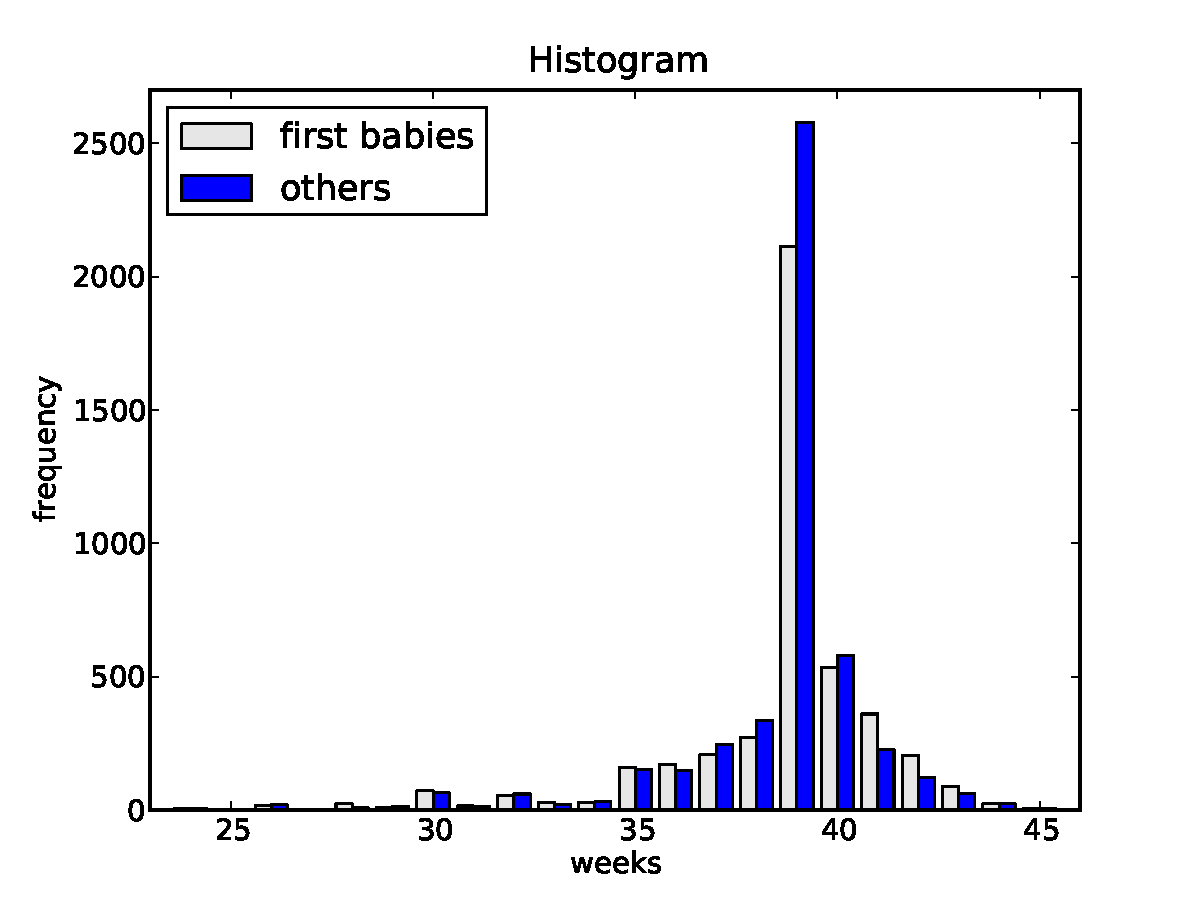
\includegraphics[height=2.5in]{figs/nsfg_hist.pdf}}
\caption{Histogram of pregnancy lengths.}
\label{nsfg_hist}
\end{figure}

Histograms are useful because they make the following features immediately
apparent:

\begin{description}

\item[Mode:] The most common value in a distribution is called the
  {\bf mode}.  In Figure~\ref{nsfg_hist} there is a clear mode at 39
  weeks.  In this case, the mode is the summary statistic that does
  the best job of describing the typical value.
\index{mode}

\item[Shape:] Around the mode, the distribution is asymmetric; it
  drops off quickly to the right and more slowly to the left.  From a
  medical point of view, this makes sense.  Babies are often born
  early, but seldom later than 42 weeks.  Also, the right side of the
  distribution is truncated because doctors often intervene after 42
  weeks.
\index{shape}

\item[Outliers:] Values far from the mode are called {\bf outliers}.
  Some of these are just unusual cases, like babies born at 30 weeks.
  But many of them are probably due to errors, either in the reporting
  or recording of data.
\index{outlier}

\end{description}

Although histograms make some features apparent, they are usually not
useful for comparing two distributions.  In this example, there are
fewer ``first babies'' than ``others,'' so some of the apparent
differences in the histograms are due to sample sizes.  We can
address this problem using PMFs.


\section{Representing PMFs}
\index{Pmf object}
\index{{\tt pmf.py}@{\tt Pmf.py}}

{\tt Pmf.py} provides a class called {\tt Pmf} that represents PMFs.
The notation can be confusing, but here it is: {\tt Pmf} is the
name of the module and also the class, so the full name of the class
is {\tt Pmf.Pmf}.  I often use {\tt pmf} as a variable name.
Finally, in the text, I use PMF to refer to the general concept
of a probability mass function, independent of my implementation.

To create a Pmf object, use {\tt MakePmfFromList}, which takes a list
of values:
%
\begin{verbatim}
>>> import Pmf
>>> pmf = Pmf.MakePmfFromList([1, 2, 2, 3, 5])
>>> print pmf
<Pmf.Pmf object at 0xb76cf68c>
\end{verbatim}

Pmf and Hist objects are similar in many ways.  The methods {\tt
  Values} and {\tt Items} work the same way for both types.  The
biggest difference is that a Hist maps from values to integer
counters; a Pmf maps from values to floating-point probabilities.

To look up the probability associated with a value, use {\tt Prob}:
%
\begin{verbatim}
>>> pmf.Prob(2)
0.4
\end{verbatim}

You can modify an existing Pmf by incrementing the probability
associated with a value:
%
\begin{verbatim}
>>> pmf.Incr(2, 0.2)
>>> pmf.Prob(2)
0.6
\end{verbatim}

Or you can multiply a probability by a factor:
%
\begin{verbatim}
>>> pmf.Mult(2, 0.5)
>>> pmf.Prob(2)
0.3
\end{verbatim}

If you modify a Pmf, the result may not be normalized; that is, the
probabilities may no longer add up to 1.  To check, you can call {\tt
  Total}, which returns the sum of the probabilities:
%
\begin{verbatim}
>>> pmf.Total()
0.9
\end{verbatim}

To renormalize, call {\tt Normalize}:
%
\begin{verbatim}
>>> pmf.Normalize()
>>> pmf.Total()
1.0
\end{verbatim}

Pmf objects provide a {\tt Copy} method so you can make and
and modify a copy without affecting the original.

\begin{exercise}
According to Wikipedia, ``Survival analysis is a branch of statistics
which deals with death in biological organisms and failure in
mechanical systems;'' see \url{http://wikipedia.org/wiki/Survival_analysis}.
\index{survival analysis}

As part of survival analysis, it is often useful to compute the
remaining lifetime of, for example, a mechanical component.  If we
know the distribution of lifetimes and the age of the component,
we can compute the distribution of remaining lifetimes.

Write a function called {\tt RemainingLifetime} that takes a
Pmf of lifetimes and an age, and returns a new Pmf that represents
the distribution of remaining lifetimes.

\end{exercise}


\begin{exercise}
%
\index{mean}
\index{variance}
\index{PMF}
%
In Section~\ref{mean} we computed the mean of a sample by adding up
the elements and dividing by \n.  If you are given a PMF, you can
still compute the mean, but the process is slightly different:
%
\[ \mu = \sum_i p_i x_i \]
%
where the \xsubi~are the unique values in the PMF and \psubi=PMF(\xsubi).
Similarly, you can compute variance like this:
%
\[ \sigma^2 = \sum_i p_i (x_i - \mu)^2\]
% 
Write functions called {\tt PmfMean} and {\tt PmfVar} that take a
Pmf object and compute the mean and variance.  To test these methods,
check that they are consistent with the methods {\tt Mean} and {\tt
  Var} in {\tt Pmf.py}.
\index{{\tt pmf.py}@{\tt Pmf.py}}

\end{exercise}




\section{Plotting PMFs}
\index{plotting}
\index{PMF}

There are two common ways to plot Pmfs:

\begin{itemize}

\item To plot a Pmf as a bar graph, you can use {\tt pyplot.bar}
or {\tt myplot.Hist}.  Bar graphs are most useful if the number
of values in the Pmf is small.
\index{bar plot}
\index{plot!bar}

\item To plot a Pmf as a line, you can use {\tt pyplot.plot}
or {\tt myplot.Pmf}.  Line plots are most useful if there are
a large number of values and the Pmf is smooth.
\index{line plot}
\index{plot!line}

\end{itemize}

\begin{figure}
% descriptive.py
\centerline{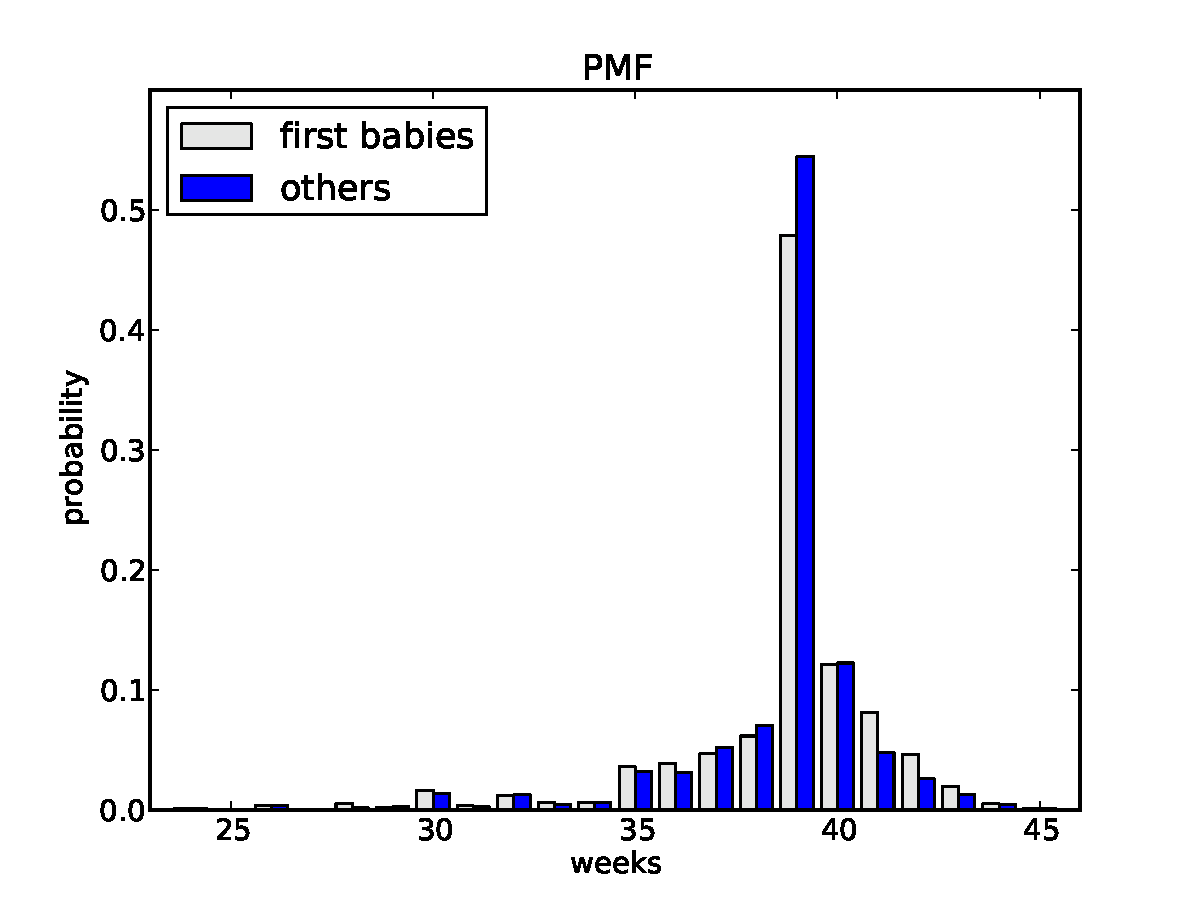
\includegraphics[height=2.5in]{figs/nsfg_pmf.pdf}}
\caption{PMF of pregnancy lengths.}
\label{nsfg_pmf}
\end{figure}
\index{pregnancy length}
\index{length!pregnancy}

Figure~\ref{nsfg_pmf} shows the PMF of pregnancy lengths as a bar
graph.  Using the PMF, we can see more clearly where the distributions
differ.  First babies seem to be less likely to arrive on time (week
39) and more likely to be a late (weeks 41 and 42).

The code that generates the figures in this chapters is available from
\url{http://thinkstats.com/descriptive.py}.  To run it, you will need the
modules it imports and the data from the NSFG (see
Section~\ref{nsfg}).
\index{National Survey of Family Growth}
\index{NSFG}
\index{{\tt descriptive.py}}

Note: {\tt pyplot} provides a function called {\tt hist} that
takes a sequence of values, computes the histogram and plots it.
Since I use {\tt Hist} objects, I usually don't use {\tt pyplot.hist}.


\section{Outliers}
\index{outlier}

Outliers are values that are far from the central tendency.  Outliers
might be caused by errors in collecting or processing the data, or
they might be correct but unusual measurements.  It is always a good
idea to check for outliers, and sometimes it is useful and appropriate
to discard them.

%weeks  count
%0      1
%4      1
%9      1
%13     1
%17     2
%18     1
%19     1
%20     1
%21     2
%22     7

In the list of pregnancy lengths for live births, the 10 lowest values
are \{0, 4, 9, 13, 17, 17, 18, 19, 20, 21\}.  Values below 20
weeks are certainly errors, and values higher than 30 weeks are
probably legitimate.  But values in between are
hard to interpret.
\index{pregnancy length}
\index{length!pregnancy}

On the other end, the highest values are:
%
\begin{verbatim}
weeks  count
43     148
44     46
45     10
46     1
47     1
48     7
50     2
\end{verbatim}

Again, some values are almost certainly errors,
but it is hard to know for sure.  One option is to {\bf trim} the data
by discarding some fraction of the highest and lowest values (see
\url{http://wikipedia.org/wiki/Truncated_mean}).
\index{trimmed mean}
\index{mean!trimmed}
\index{truncated mean}
\index{mean!truncated}


\section{Other visualizations}
\index{visualization}
\index{exploratory data analysis}

Histograms and PMFs are useful for exploratory data analysis;
once you have an idea what is going on, it is often useful to
design a visualization that focuses on the apparent effect.
\index{apparent effect}

In the NSFG data, the biggest differences in the distributions are
near the mode.  So it makes sense to zoom in on that part of the
graph, and to transform the data to emphasize differences.
\index{National Survey of Family Growth}
\index{NSFG}

Figure~\ref{nsfg_diffs} shows the difference between the PMFs for weeks
35--45.  I multiplied by 100 to express the differences in percentage
points.

\begin{figure}
% descriptive.py
\centerline{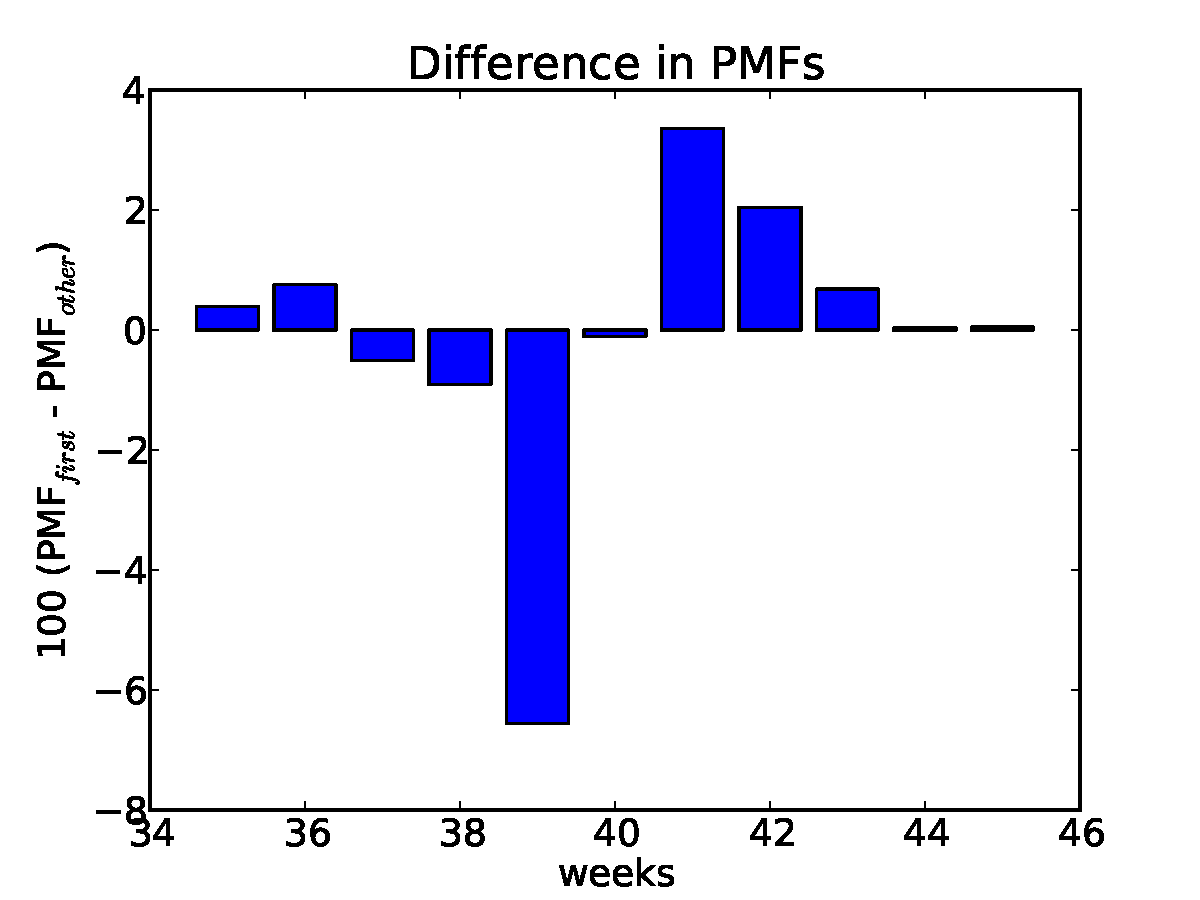
\includegraphics[height=2.5in]{figs/nsfg_diffs.pdf}}
\caption{Difference in percentage, by week.}
\label{nsfg_diffs}
\end{figure}

This figure makes the pattern clearer: first babies are
less likely to be born in week 39, and somewhat more likely
to be born in weeks 41 and 42.


\section{Relative risk}
\label{relative.risk}
\index{relative risk}

We started with the question, ``Do first babies arrive late?''  To
make that more precise, let's say that a baby is early if it is born
during Week 37 or earlier, on time if it is born during Week 38, 39 or
40, and late if it is born during Week 41 or later.  Ranges like these
that are used to group data are called {\bf bins}.
\index{bin}
\index{{\tt risk.py}}

\begin{exercise}
Create a file named {\tt risk.py}.
Write functions named {\tt ProbEarly}, {\tt ProbOnTime} and
{\tt ProbLate} that take a PMF and compute the fraction of births
that fall into each bin.  Hint: write a generalized function
that these functions call.

Make three PMFs, one for first babies, one for others, and one for
all live births.  For each PMF, compute the probability of being
born early, on time, or late.

One way to summarize data like this is with {\bf relative risk},
which is a ratio of two probabilities.  For example, the probability
that a first baby is born early is 18.2\%.  For other babies it is
16.8\%, so the relative risk is 1.08.  That means that first babies
are about 8\% more likely to be early.

Write code to confirm that result, then compute the relative risks of
being born on time and being late.  You can download a solution
from \url{http://thinkstats.com/risk.py}.

\end{exercise}


\section{Conditional probability}
\index{conditional probability}
\index{probability!conditional}

Imagine that someone you know is pregnant, and it is the beginning of
Week 39.  What is the chance that the baby will be born in the next
week?  How much does the answer change if it's a first baby?

We can answer these questions by computing a {\bf conditional
probability}, which is (ahem!) a probability that depends on a condition.
In this case, the condition is that we know the baby didn't arrive
during Weeks 0--38.

Here's one way to do it:

\begin{enumerate}

\item Given a PMF, generate a fake cohort of 1000 pregnancies.
For each number of weeks, \x, the number of pregnancies with
duration \x~is 1000 PMF(\x).
\index{cohort}

\item Remove from the cohort all pregnancies with length less than 39.
\index{pregnancy length}
\index{length!pregnancy}

\item Compute the PMF of the remaining durations; the result is the
conditional PMF.

\item Evaluate the conditional PMF at \x~=~39 weeks.

\end{enumerate}

This algorithm is conceptually clear, but not very efficient.
A simple alternative is to remove from the distribution the values
less than 39 and then renormalize.

\begin{exercise}
Write a function that implements either of these algorithms and
computes the probability that a baby will be born during Week 39,
given that it was not born prior to Week 39.

Generalize the function to compute the
probability that a baby will be born during Week \x, given that
it was not born prior to Week \x, for all \x.
Plot this value as a function of \x~for first babies and others.

You can download a solution to this problem from
\url{http://thinkstats.com/conditional.py}.
\index{{\tt conditional.py}}

\end{exercise}


\section{Reporting results}

At this point we have explored the data and seen several apparent
effects.  For now, let's assume that these effects are real (but let's
remember that it's an assumption).  How should we report these
results?

The answer might depend on who is asking the question.  For example, a
scientist might be interested in any (real) effect, no matter how
small.  A doctor might only care about effects that are {\bf
  clinically significant}; that is, differences that affect treatment
decisions.  A pregnant woman might be interested in results that are
relevant to her, like the conditional probabilities in the previous
section.
\index{clinically significant}
\index{significance}

How you report results also depends on your goals.  If you are
trying to demonstrate the significance of an effect, you might choose
summary statistics, like relative risk, that emphasize differences.
If you are trying to reassure a patient, you might choose statistics
that put the differences in context.

\begin{exercise}
Based on the results from the previous exercises, suppose you were
asked to summarize what you learned about whether first
babies arrive late.

Which summary statistics would you use if you wanted to get a story
on the evening news?  Which ones would you use if you wanted to
reassure an anxious patient?
\index{Adams, Cecil}
\index{Straight Dope, The}

Finally, imagine that you are Cecil Adams, author of {\it The Straight
  Dope} (\url{http://straightdope.com}), and your job is to answer the
question, ``Do first babies arrive late?''  Write a paragraph that
uses the results in this chapter to answer the question clearly,
precisely, and accurately.

\end{exercise}



\section{Glossary}

\begin{description}

\item[central tendency:] A characteristic of a sample or population;
intuitively, it is the most average value. 
\index{central tendency}

\item[spread:] A characteristic of a sample or population;
intuitively, it describes how much variability there is.
\index{spread}

\item[variance:] A summary statistic often used to quantify spread.
\index{variance}

\item[standard deviation:] The square root of variance, also used
as a measure of spread.
\index{standard deviation}

\item[frequency:] The number of times a value appears in a sample.
\index{frequency}

\item[histogram:] A mapping from values to frequencies, or a graph
that shows this mapping.
\index{histogram}

\item[probability:] A frequency expressed as a fraction of the sample
size.
\index{probability}

\item[normalization:] The process of dividing a frequency by a sample
size to get a probability.
\index{normalization}

\item[distribution:] A summary of the values that appear in a sample
and the frequency, or probability, of each.
\index{distribution}

\item[PMF:] Probability mass function: a representation of a distribution
as a function that maps from values to probabilities.
\index{PMF}

\item[mode:] The most frequent value in a sample.
\index{mode}

\item[outlier:] A value far from the central tendency.
\index{outlier}

\item[trim:] To remove outliers from a dataset.
\index{trim}

\item[bin:] A range used to group nearby values.
\index{bin}

\item[relative risk:] A ratio of two probabilities, often used to measure
a difference between distributions.
\index{relative risk}

\item[conditional probability:] A probability computed under the assumption
that some condition holds.
\index{conditional probability}

\item[clinically significant:] A result, like a difference between groups,
that is relevant in practice.
\index{clinically significant}

\end{description}


\chapter{Cumulative distribution functions}
\label{cumulative}

\section{The class size paradox}
\index{class size}

At many American colleges and universities, the student-to-faculty
ratio is about 10:1.  But students are often surprised to discover
that their average class size is bigger than 10.  There
are two reasons for the discrepancy:

\begin{itemize}

\item Students typically take 4--5 classes per semester, but
professors often teach 1 or 2.

\item The number of students who enjoy a small class is small,
but the number of students in a large class is (ahem!) large.

\end{itemize}

The first effect is obvious (at least once it is pointed out);
the second is more subtle.  So let's look at an example.  Suppose
that a college offers 65 classes in a given semester, with the
following distribution of sizes:
%
\begin{verbatim}
 size      count
 5- 9          8
10-14          8
15-19         14
20-24          4
25-29          6
30-34         12
35-39          8
40-44          3
45-49          2
\end{verbatim}

If you ask the Dean for the average class size, he would
construct a PMF, compute the mean, and report that the
average class size is 24.

But if you survey a group of students, ask them how many
students are in their classes, and compute the mean, you would
think that the average class size was higher.

\begin{exercise}
Build a PMF of these data and compute the mean as perceived by the
Dean.  Since the data have been grouped in bins, you can use the
mid-point of each bin.
\index{PMF}

Now find the distribution of class sizes as perceived by students
and compute its mean.  

Suppose you want to find the distribution of class sizes at a
college, but you can't get reliable data from the Dean.
An alternative is to choose a random sample of students and ask them
the number of students in each of their classes.  Then you could compute
the PMF of their responses.
\index{bias!oversampling}
\index{oversampling}

The result would be biased because large classes
would be oversampled, but you could estimate the actual
distribution of class sizes by applying an appropriate transformation
to the observed distribution.

Write a function called \verb"UnbiasPmf" that takes the PMF of the
observed values and returns a new Pmf object that estimates the
distribution of class sizes.

You can download a solution to this problem from
\url{http://thinkstats.com/class_size.py}.
\index{{\tt class\_size.py}}

\end{exercise}


\begin{exercise}
\label{relay}

In most foot races, everyone starts at the same time.  If you are a
fast runner, you usually pass a lot of people at the beginning of the
race, but after a few miles everyone around you is going at the same
speed.
\index{relay race}
\index{bias!oversampling}
\index{oversampling}

When I ran a long-distance (209 miles) relay race for the first
time, I noticed an odd phenomenon: when I overtook another runner, I
was usually much faster, and when another runner overtook me, he was
usually much faster.

At first I thought that the distribution of speeds might be bimodal;
that is, there were many slow runners and many fast runners, but few
at my speed.

Then I realized that I was the victim of selection bias.  The race
was unusual in two ways: it used a staggered start, so teams started
at different times; also, many teams included runners at different
levels of ability.
\index{bias!selection}
\index{selection bias}

As a result, runners were spread out along the course with little
relationship between speed and location.  When I started running my
leg, the runners near me were (pretty much) a random sample of the
runners in the race.

So where does the bias come from?  During my time on the course, the
chance of overtaking a runner, or being overtaken, is proportional to
the difference in our speeds.  To see why, think about the extremes.
If another runner is going at the same speed as me, neither of us will
overtake the other.  If someone is going so fast that they cover the
entire course while I am running, they are certain to overtake me.

Write a function called {\tt BiasPmf} that takes a Pmf representing
the actual distribution of runners' speeds, and the speed of a running
observer, and returns a new Pmf representing the distribution of
runners' speeds as seen by the observer.

To test your function, get the distribution of speeds from a
normal road race (not a relay).  I wrote a program that reads the
results from the James Joyce Ramble 10K in Dedham MA and converts the
pace of each runner to MPH.  Download it from
\url{http://thinkstats.com/relay.py}.  Run it and look at the PMF of
speeds.
\index{{\tt relay.py}}
\index{{\tt relay\_soln.py}}

Now compute the distribution of speeds you would observe if you ran a
relay race at 7.5 MPH with this group of runners.  You can download a
solution from \url{http://thinkstats.com/relay_soln.py}

\end{exercise}


\section{The limits of PMFs}
\index{PMF}

PMFs work well if the number of values is small.  But as the
number of values increases, the probability associated with each value
gets smaller and the effect of random noise increases.

For example, we might be interested in the distribution of birth
weights.  In the NSFG data, the variable \verb"totalwgt_oz" records
weight at birth in ounces.  Figure~\ref{nsfg_birthwgt_pmf} shows the
PMF of these values for first babies and others.
\index{National Survey of Family Growth}
\index{NSFG}
\index{birth weight}
\index{weight!birth}

\begin{figure}
% cumulative.py
\centerline{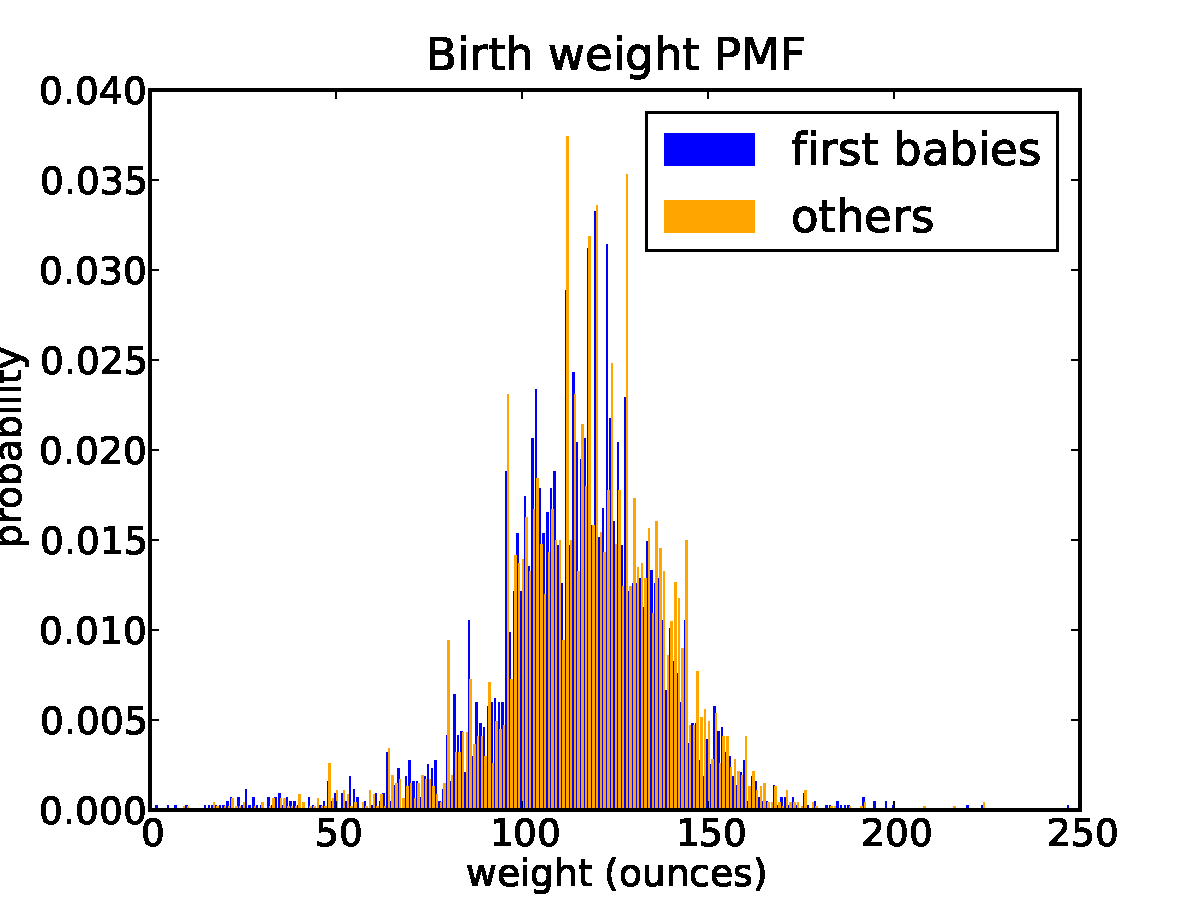
\includegraphics[height=2.5in]{figs/nsfg_birthwgt_pmf.pdf}}
\caption{PMF of birth weights.  This figure shows a limitation
of PMFs: they are hard to compare.}
\label{nsfg_birthwgt_pmf}
\end{figure}

Overall, these distributions resemble the familiar ``bell curve,'' with
many values near the mean and a few values much higher and lower.

But parts of this figure are hard to interpret.  There are many spikes
and valleys, and some apparent differences between the distributions.
It is hard to tell which of these features are significant.  Also, it
is hard to see overall patterns; for example, which distribution do
you think has the higher mean?
\index{binning}

These problems can be mitigated by binning the data;
that is, dividing the domain into non-overlapping intervals and counting
the number of values in each bin.  Binning can be useful, but it is
tricky to get the size of the bins right.  If they are big enough to
smooth out noise, they might also smooth out useful information.

An alternative that avoids these problems is the {\bf cumulative
distribution function}, or {\bf CDF}.  But before we can get to that,
we have to talk about percentiles.
\index{cumulative distribution function}
\index{CDF}


\section{Percentiles}
\index{percentile rank}

If you have taken a standardized test, you probably got your
results in the form of a raw score and a {\bf percentile rank}.
In this context, the percentile rank is the fraction of people who
scored lower than you (or the same).  So if you are ``in the 90th
percentile,'' you did as well as or better than 90\% of the people who
took the exam.

Here's how you could compute the percentile rank of a value,
\verb"your_score", relative to the scores in the sequence {\tt
  scores}:
%
\begin{verbatim}
def PercentileRank(scores, your_score):
    count = 0
    for score in scores:
        if score <= your_score:
            count += 1

    percentile_rank = 100.0 * count / len(scores)
    return percentile_rank
\end{verbatim}
%
% see score_example.py
%
For example, if the scores in the sequence were 55, 66, 77, 88 and 99,
and you got the 88, then your percentile rank would be {\tt 100 * 4 / 5}
which is 80.

If you are given a value, it is easy to find its percentile rank; going
the other way is slightly harder.  If you are given a percentile rank
and you want to find the corresponding value, one option is to
sort the values and search for the one you want:
%
\begin{verbatim}
def Percentile(scores, percentile_rank):
    scores.sort()
    for score in scores:
        if PercentileRank(scores, score) >= percentile_rank:
            return score
\end{verbatim}

The result of this calculation is a {\bf percentile}.  For example,
the 50th percentile is the value with percentile rank 50.  In the
distribution of exam scores, the 50th percentile is 77.
\index{percentile}

\begin{exercise}
This implementation of {\tt Percentile} is not very efficient.  A
better approach is to use the percentile rank to compute the index of
the corresponding percentile.  Write a version of {\tt Percentile} that
uses this algorithm.

You can download a solution from \url{http://thinkstats.com/score_example.py}.
\index{{\tt score\_example.py}}

\end{exercise}

\begin{exercise}
Optional: If you only want to compute one percentile, it is not
efficient to sort the scores.  A better option is the selection
algorithm, which you can read about at
\url{http://wikipedia.org/wiki/Selection_algorithm}.
\index{selection algorithm}

Write (or find) an implementation of the selection algorithm and use
it to write an efficient version of {\tt Percentile}.

\end{exercise}


\section{Cumulative distribution functions}
\index{cumulative distribution function}
\index{CDF}

Now that we understand percentiles, we are ready to tackle the
cumulative distribution function (CDF).  The CDF is the function that
maps values to their percentile rank in a distribution.

The CDF is a function of \x, where \x~is any value that might appear
in the distribution.  To evaluate CDF(\x) for a particular value of
\x, we compute the fraction of the values in the sample less than (or
equal to) \x.

Here's what that looks like as a function that takes a sample,
{\tt t}, and a value, {\tt x}:
%
\begin{verbatim}
def Cdf(t, x):
    count = 0.0
    for value in t:
        if value <= x:
            count += 1.0

    prob = count / len(t)
    return prob
\end{verbatim}

This function should look familiar; it is almost identical to {\tt
  PercentileRank}, except that the result is in a probability in the
range 0--1 rather than a percentile rank in the range 0--100.

As an example, suppose a sample has the values \{1, 2, 2, 3, 5\}.
Here are some values from its CDF:

\Eqn{ CDF(0)~=~0  }

\Eqn{ CDF(1)~=~0.2 }

\Eqn{ CDF(2)~=~0.6 }

\Eqn{ CDF(3)~=~0.8 }

\Eqn{ CDF(4)~=~0.8 }

\Eqn{ CDF(5)~=~1 }

We can evaluate the CDF for any value of \x, not just
values that appear in the sample.
If \x~is less than the smallest value in the sample, CDF(\x) is 0.
If \x~is greater than the largest value, CDF(\x) is 1.

\begin{figure}
% cumulative.py
\centerline{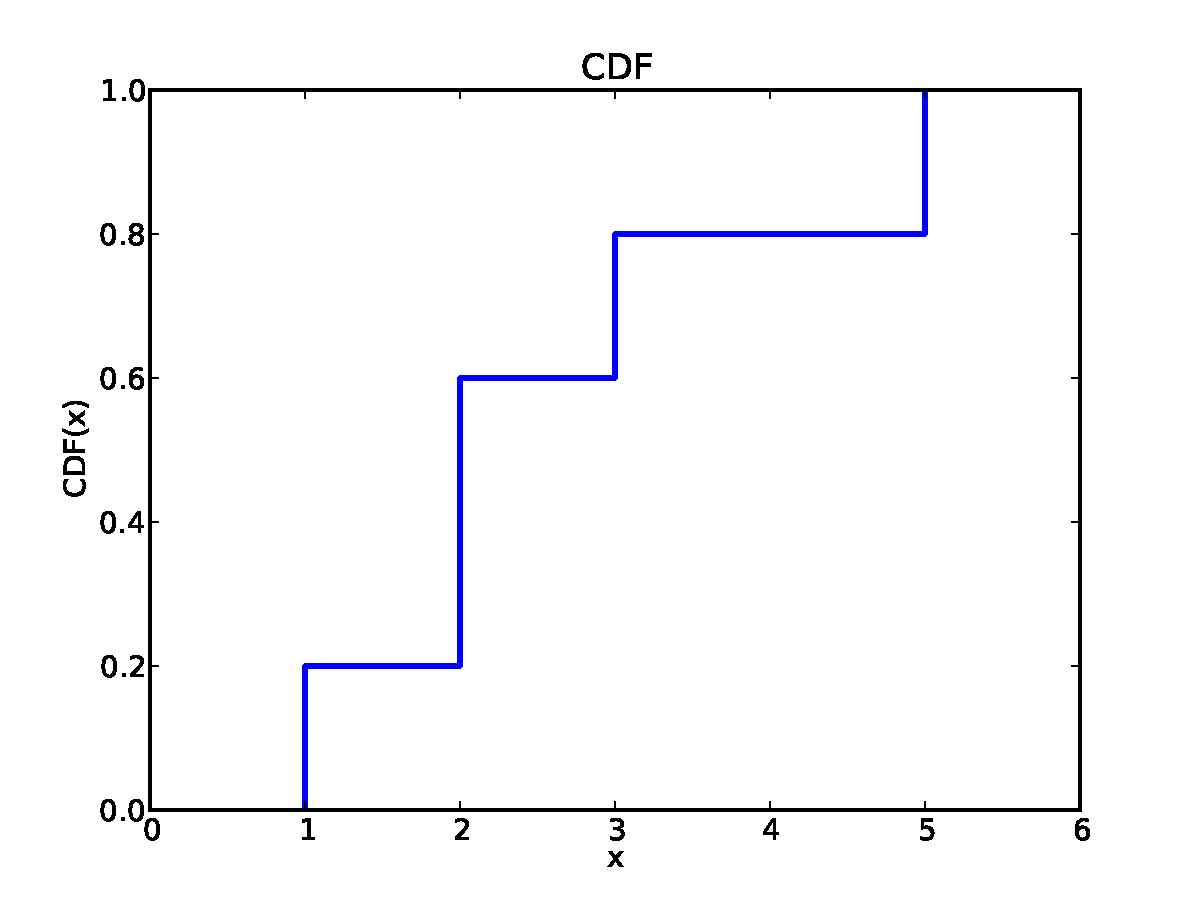
\includegraphics[height=2.5in]{figs/example_cdf.pdf}}
\caption{Example of a CDF.}
\label{example_cdf}
\end{figure}

Figure~\ref{example_cdf} is a graphical representation of this CDF.
The CDF of a sample is a step function.  In the next chapter we
will see distributions whose CDFs are continuous functions.  


\section{Representing CDFs}
\index{{\tt cdf.py}@{\tt Cdf.py}}
\index{Cdf object}

I have written a module called {\tt Cdf} that provides a class named
{\tt Cdf} that represents CDFs.  You can read the documentation of
this module at \url{http://thinkstats.com/Cdf.html} and you can download it
from \url{http://thinkstats.com/Cdf.py}.

Cdfs are implemented with two sorted lists: {\tt xs}, which contains
the values, and {\tt ps}, which contains the probabilities.  The
most important methods Cdfs provide are:

\begin{description}

\item[{\tt Prob(x)}:] Given a value \x, computes the probability \p~=~CDF(\x).

\item[{\tt Value(p)}:] Given a probability \p, computes the
corresponding value, \x; that is, the inverse CDF of \p.

\end{description}

Because {\tt xs} and {\tt ps} are sorted, these operations can use the
bisection algorithm, which is efficient.  The run time is proportional
to the logarithm of the number of values; see
\url{http://wikipedia.org/wiki/Time_complexity}.
\index{bisection algorithm}

Cdfs also provide {\tt Render}, which returns two lists, {\tt xs} and
{\tt ps}, suitable for plotting the CDF.  Because the CDF is a
step function, these lists have two elements for each unique
value in the distribution.

The Cdf module provides several functions for making Cdfs, including
{\tt MakeCdfFromList}, which takes a sequence of values
and returns their Cdf.

Finally, {\tt myplot.py} provides functions named {\tt Cdf} and
{\tt Cdfs} that plot Cdfs as lines.
\index{{\tt myplot.py}}

\begin{exercise}
Download {\tt Cdf.py} and \verb"relay.py" (see
Exercise~\ref{relay}) and generate a plot that shows the CDF of
running speeds.  Which gives you a better sense of the shape of the
distribution, the PMF or the CDF?  You can download a solution
from \url{http://thinkstats.com/relay_cdf.py}.
\index{{\tt cdf.py}@{\tt Cdf.py}}
\index{{\tt relay\_cdf.py}}

\end{exercise}


\section{Back to the survey data}
\label{birth_weights}
\index{National Survey of Family Growth}
\index{NSFG}
\index{birth weight}
\index{weight!birth}

Figure~\ref{nsfg_birthwgt_cdf} shows the CDFs of birth weight for
first babies and others in the NSFG dataset.

\begin{figure}
% cumulative.py
\centerline{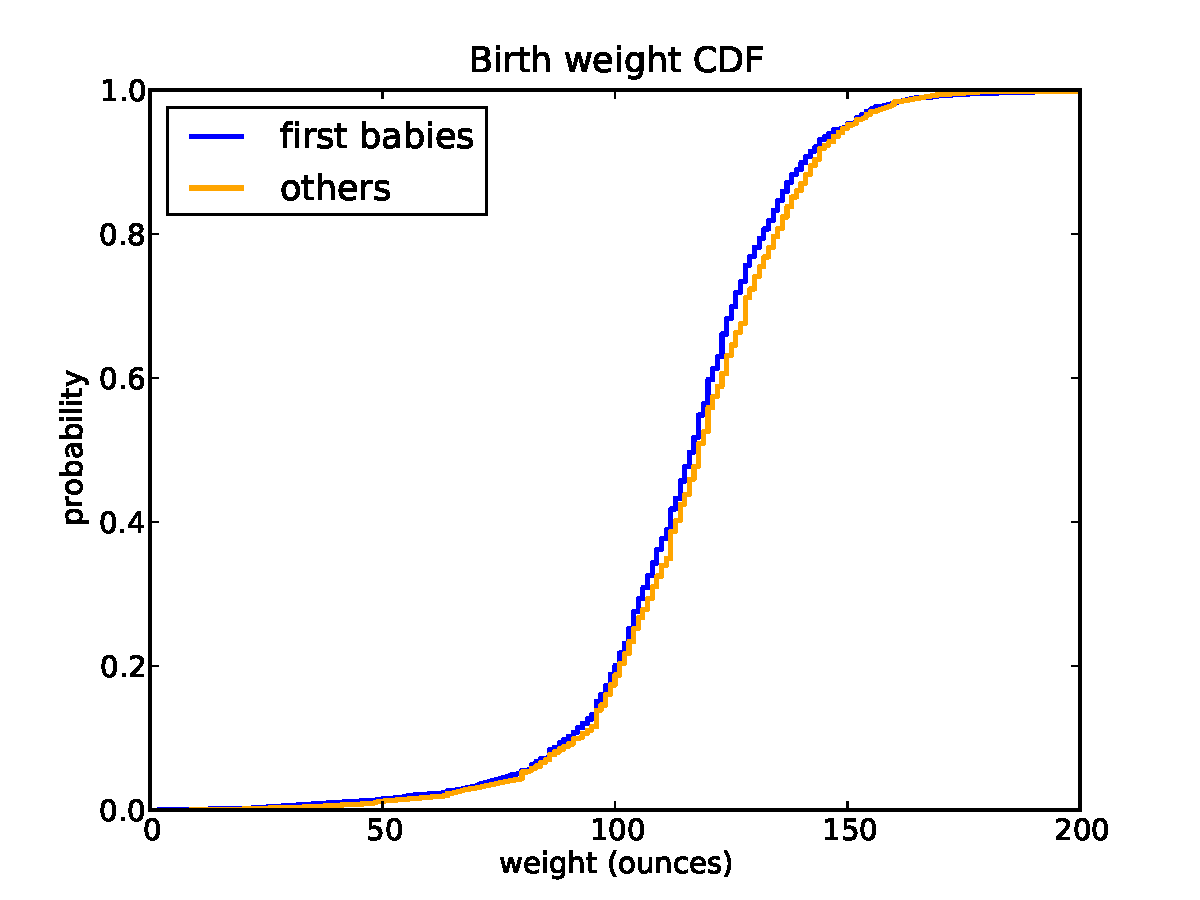
\includegraphics[height=2.5in]{figs/nsfg_birthwgt_cdf.pdf}}
\caption{CDF of birth weights.}
\label{nsfg_birthwgt_cdf}
\end{figure}

This figure makes the shape of the distributions, and the differences
between them, much clearer.  We can see that first babies are slightly
lighter throughout the distribution, with a larger discrepancy above 
the mean.
\index{shape}

%\begin{exercise}

%In the figure above, you might notice
%a sequence of equally-spaced values with higher frequency than
%their neighbors.  See if you can figure out what is going on.
%Hint: look at the PMF of \verb"birthwgt_oz".

%\end{exercise}

\begin{exercise}
How much did you weigh at birth?  If you don't know, call your mother
or someone else who knows.  Using the pooled data (all live births),
compute the distribution of birth weights and use it to find your
percentile rank.  If you were a first baby, find your percentile rank
in the distribution for first babies.  Otherwise use the distribution
for others.  How big is the difference between your percentile ranks
in the two distributions?

\end{exercise}

\begin{exercise}
Suppose you and your classmates compute the percentile rank of your
birth weights and then compute the CDF of the percentile ranks.  What do
you expect it to look like?  Hint: what fraction of the class do you
expect to be above the median?
\index{birth weight}
\index{weight!birth}

\end{exercise}


\section{Conditional distributions}
\index{conditional distribution}
\index{distribution!conditional}

A {\bf conditional distribution} is the distribution of a subset of
the data which is selected according to a condition.

For example, if you are above average in weight, but way above average
in height, then you might be relatively light for your height.  Here's
how you could make that claim more precise.

\begin{enumerate}

\item Select a cohort of people who are the same height as you (within
some range).
\index{cohort}

\item Find the CDF of weight for those people.

\item Find the percentile rank of your weight in that distribution.

\end{enumerate}

Percentile ranks are useful for comparing measurements from
different tests, or tests applied to different groups.
\index{percentile rank}
\index{rank!percentile}

For example, people who compete in foot races are usually grouped by
age and gender.  To compare people in different groups, you can convert
race times to percentile ranks.

\begin{exercise}
I recently ran the James Joyce Ramble 10K
in Dedham MA.  The results are available from
\url{http://coolrunning.com/results/10/ma/Apr25_27thAn_set1.shtml}.
Go to that page and find my results.  I came in 97th in a field
of 1633, so what is my percentile rank in the field?
\index{James Joyce Ramble}
\index{race time}

In my division (M4049 means ``male between 40 and 49 years of age'')
I came in 26th out of 256.  What is my percentile rank in my division?

If I am still running in 10 years (and I hope I am), I will be in
the M5059 division.  Assuming that my percentile rank in my division
is the same, how much slower should I expect to be?

I maintain a friendly rivalry with a student who is in the
F2039 division.  How fast does she have to run her next 10K to
``beat'' me in terms of percentile ranks?

\end{exercise}


\section{Random numbers}
\label{random}
\index{random number}

CDFs are useful for generating random numbers with a given
distribution.  Here's how:

\begin{itemize}

\item Choose a random probability in the range 0--1.

\item Use {\tt Cdf.Value} to find the value in the distribution
that corresponds to the probability you chose.

\end{itemize}

It might not be obvious why this works, but since it is easier
to implement than to explain, let's try it out.

\begin{exercise}
Write a function called {\tt Sample}, that takes a Cdf and
an integer, \n, and returns a list of \n~values chosen at
random from the Cdf.  Hint: use {\tt random.random}.
You will find a solution to this exercise in {\tt Cdf.py}.
\index{inverse CDF algorithm}
\index{{\tt cdf.py}@{\tt Cdf.py}}

Using the distribution of birth weights from the NSFG, generate a
random sample with 1000 elements.  Compute the CDF of the sample.
Make a plot that shows the original CDF and the CDF of the random
sample.  For large values of \n, the distributions should be
the same.
\index{birth weight}
\index{weight!birth}
\index{National Survey of Family Growth}
\index{NSFG}

\end{exercise}

This process, generating a random sample based on a measured sample,
is called {\bf resampling}.
\index{resampling}
\index{sampling}
\index{replacement, sampling}

There are two ways to draw a sample from a population: with and
without replacement.  If you imagine drawing marbles from an
urn\footnote{The marbles-in-an-urn scenario is a standard model for
  random sampling processes (see
  \url{http://wikipedia.org/wiki/Urn_problem}).}, ``replacement'' means
putting the marbles back as you go (and stirring), so the population
is the same for every draw.  ``Without replacement,'' means that each
marble can only be drawn once, so the remaining population is
different after each draw.

In Python, sampling with replacement can be implemented with
{\tt random.random} to choose a percentile rank, or {\tt random.choice}
to choose an element from a sequence.  Sampling without replacement
is provided by {\tt random.sample}.
\index{random module}

\begin{exercise}
The numbers generated by {\tt random.random} are supposed to be
uniform between 0 and 1; that is, every value in the range
should have the same probability.

Generate 1000 numbers from {\tt random.random} and plot their
PMF and CDF.  Can you tell whether they are uniform?

You can read about the uniform distribution at
\url{http://wikipedia.org/wiki/Uniform_distribution_(discrete)}.
\index{uniform distribution}
\index{distribution!uniform}

\end{exercise}


\section{Summary statistics revisited}
\index{summary statistic}
\index{interquartile range}
\index{quartile}
\index{percentile}
\index{median}
\index{central tendency}
\index{spread}

Once you have computed a CDF, it is easy to compute other summary
statistics.  The median is just the 50th percentile\footnote{You might
see other definitions of the median.  In particular,
some sources suggest that if you have an even number of elements in
a sample, the median is the average of the middle two elements.
This is an unnecessary special case, and it has the odd effect of
generating a value that is not in the sample.  As far
as I'm concerned, the median is the 50th percentile.  Period.}.
The 25th and 75th percentiles are often used to check whether
a distribution is symmetric, and their difference, which is called
the {\bf interquartile range}, measures the spread.

\begin{exercise}
Write a function called {\tt Median} that takes a Cdf and computes the
median, and one called {\tt Interquartile} that computes
the interquartile range.

Compute the 25th, 50th, and 75th percentiles of the birth weight
CDF.  Do these values suggest that the distribution is symmetric?
\index{symmetric}
\index{birth weight}
\index{weight!birth}

\end{exercise}


\section{Glossary}

\begin{description}

\item[percentile rank:] The percentage of values in a distribution that are
less than or equal to a given value.
\index{percentile rank}

\item[CDF:] Cumulative distribution function, a function that maps
  from values to their percentile ranks.
\index{CDF}

\item[percentile:] The value associated with a given percentile rank.
\index{percentile}

\item[conditional distribution:] A distribution computed under the assumption
that some condition holds.
\index{conditional distribution}

\item[resampling:] The process of generating a random sample from a
distribution that was computed from a sample.
\index{resampling}

\item[replacement:] During a sampling process, ``replacement'' indicates
that the population is the same for every sample.  ``Without replacement''
indicates that each element can be selected only once.
\index{replacement}

\item[interquartile range:] A measure of spread, the difference between
the 75th and 25th percentiles.
\index{interquartile range}

\end{description}



\chapter{Continuous distributions}
\label{continuous}
\index{continuous distribution}
\index{distribution!continuous}
\index{empirical distribution}
\index{distribution!empirical}

The distributions we have used so far are called {\bf
  empirical distributions} because they are based on empirical
observations, which are necessarily finite samples.

The alternative is a {\bf continuous distribution}, which is
characterized by a CDF that is a continuous function (as opposed to a
step function).  Many real world phenomena can be approximated by
continuous distributions.

\section{The exponential distribution}
\index{exponential distribution}
\index{distribution!exponential}

I'll start with the exponential distribution because it is
easy to work with.  In the real world, exponential distributions
come up when we look at a series of events and measure the
times between events, which are called {\bf interarrival times}.
If the events are equally likely to occur at any time, the distribution
of interarrival times tends to look like an exponential distribution.
\index{interarrival time}

The CDF of the exponential distribution is:
%
\[ CDF(x) = 1 - e^{-\lambda x} \]
%
The parameter, \mylambda, determines the shape of the
distribution.  Figure~\ref{expo_cdf} shows what this CDF looks like with
\mylambda~=~2.
\index{parameter}


\begin{figure}
% continuous.py
\centerline{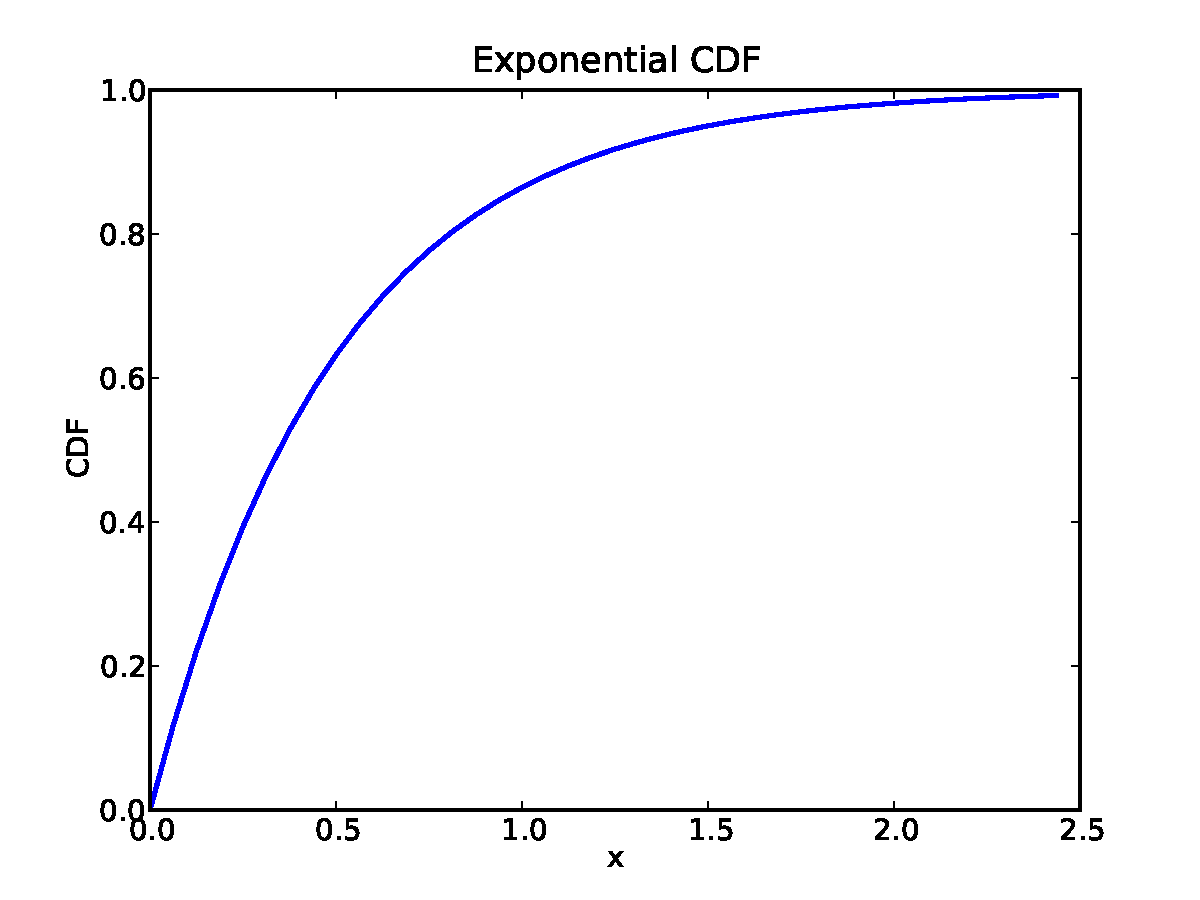
\includegraphics[height=2.5in]{figs/expo_cdf.pdf}}
\caption{CDF of exponential distribution.}
\label{expo_cdf}
\end{figure}

In general, the mean of an exponential distribution is 1\mydivide
\mylambda, so the mean of this distribution is 0.5.  The median is
log(2)\mydivide\mylambda, which is roughly 0.35.  \index{mean}
\index{median} \index{Australia} \index{Brisbane}

To see an example of a distribution that is approximately exponential,
we will look at the interarrival time of babies.
On December 18, 1997, 44 babies were born in a hospital in Brisbane,
Australia\footnote{This example is based on information and data from
  Dunn, ``A Simple Dataset for Demonstrating Common Distributions,''
  Journal of Statistics Education v.7, n.3 (1999).}.  The times of
birth for all 44 babies were reported in the local paper; you can
download the data from \url{http://thinkstats.com/babyboom.dat}.
\index{birth time}

Figure~\ref{interarrival_cdf} shows the CDF of the interarrival times
in minutes.  It seems to have the general shape of an exponential
distribution, but how can we tell?
\index{complementary CDF}
\index{CDF!complementary}
\index{CCDF}

One way is to plot the complementary CDF, 1~\minus~CDF(\x), on a
log-\y~scale.  For data from an exponential distribution, the result
is a straight line.  Let's see why that works.

If you plot the complementary CDF (CCDF) of a dataset that you think is
exponential, you expect to see a function like:
%
\[ y \approx e^{-\lambda x} \]
%
Taking the log of both sides yields:

\Eqn{ log \y~\myapprox~-\mylambda \x }

So on a log-\y~scale the CCDF is a straight line
with slope \minus\mylambda.
\index{logarithmic scale}
\index{complementary CDF}
\index{CDF!complementary}
\index{CCDF}

\begin{figure}
% babyboom.py
\centerline{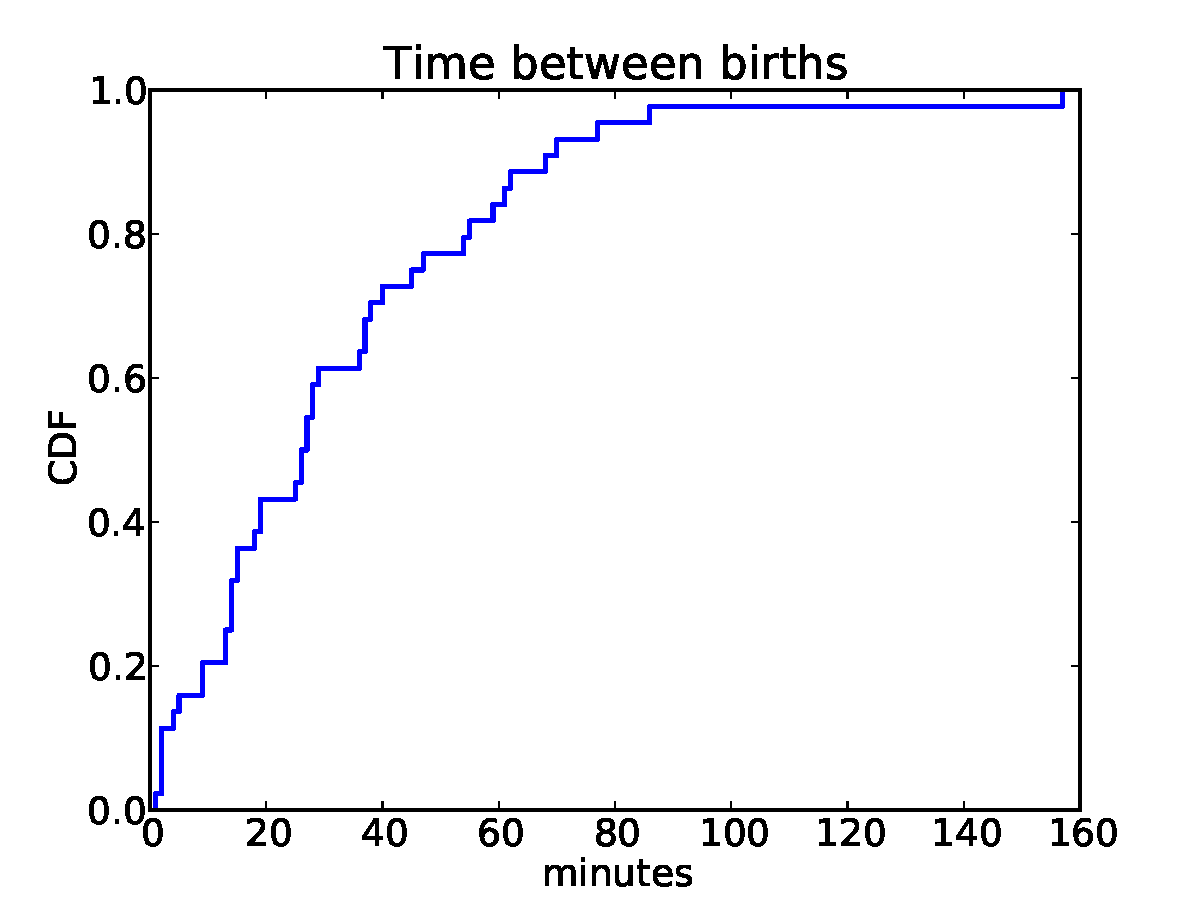
\includegraphics[height=2.5in]{figs/interarrivals.pdf}}
\caption{CDF of interarrival times}
\label{interarrival_cdf}
\end{figure}

\begin{figure}
% babyboom.py
\centerline{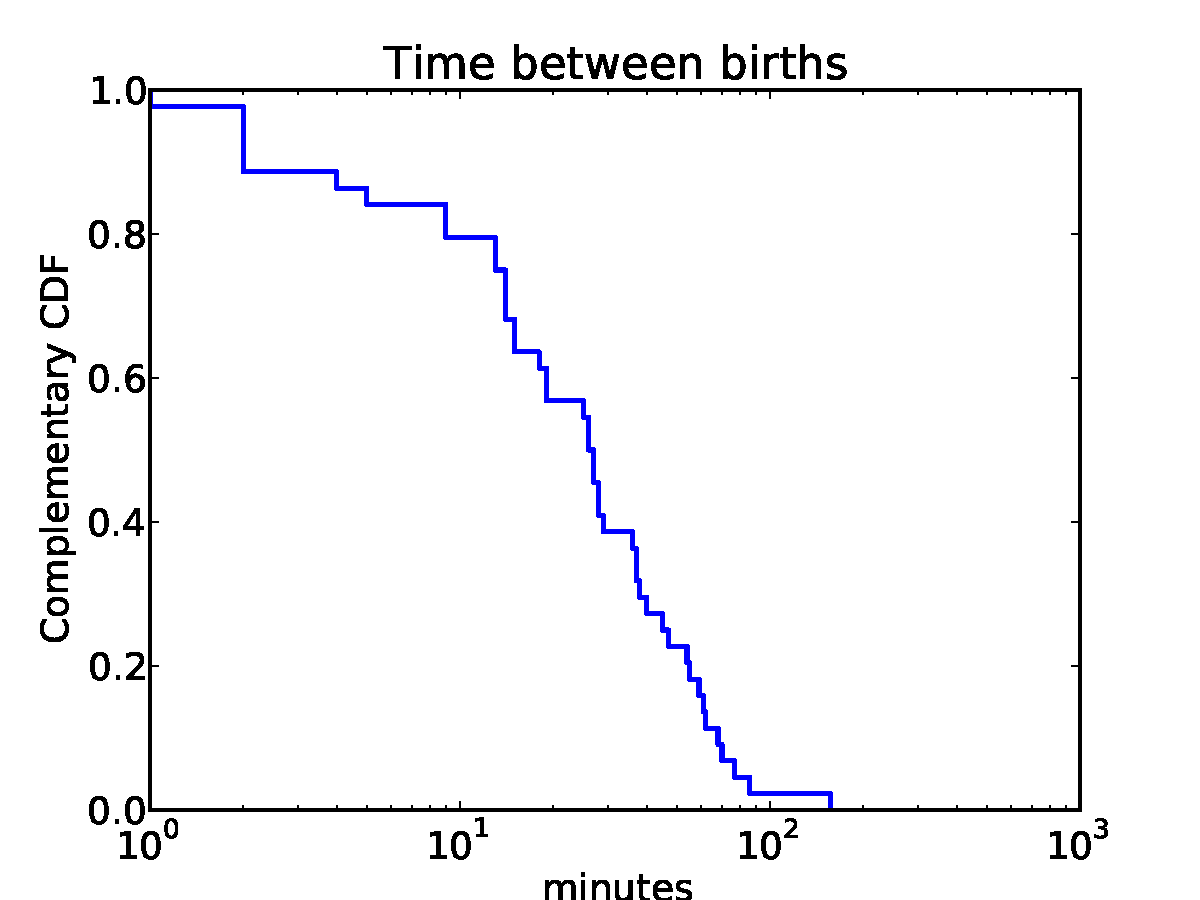
\includegraphics[height=2.5in]{figs/interarrivals_logy.pdf}}
\caption{CCDF of interarrival times.}
\label{interarrival_ccdf}
\end{figure}

Figure~\ref{interarrival_ccdf} shows the CCDF of the interarrivals
on a log-\y~scale.  It is not exactly straight, which suggests that
the exponential distribution is only an approximation.  Most likely
the underlying assumption---that a birth is equally likely at any time
of day---is not exactly true.

\begin{exercise}
For small values of \n, we don't expect an empirical distribution
to fit a continuous distribution exactly.  One way to evaluate
the quality of fit is to generate a sample from a continuous
distribution and see how well it matches the data.
\index{empirical distribution}
\index{distribution!empirical}
\index{random module}

The function {\tt expovariate} in the {\tt random} module generates
random values from an exponential distribution with a given value of
\mylambda.  Use it to generate 44 values from an exponential
distribution with mean 32.6.  Plot the CCDF on a log-\y~scale and
compare it to Figure~\ref{interarrival_ccdf}.
\index{pyplot}

Hint: You can use the function {\tt pyplot.yscale} to plot the \y~axis
on a log scale.

Or, if you use {\tt myplot}, the {\tt Cdf} function takes a boolean
option, {\tt complement}, that determines whether to plot the CDF or
CCDF, and string options, {\tt xscale} and {\tt yscale}, that
transform the axes; to plot a CCDF on a log-\y~scale:
%
\begin{verbatim}
myplot.Cdf(cdf, complement=True, xscale='linear', yscale='log') 
\end{verbatim}

\end{exercise}

\begin{exercise}
Collect the birthdays of the students in your class, sort them, and
compute the interarrival times in days.  Plot the CDF of the interarrival
times and the CCDF on a log-\y~scale.  Does it look like
an exponential distribution?
\index{exponential distribution}
\index{distribution!exponential}
\index{birthday}

\end{exercise}


\section{The Pareto distribution}
\index{Pareto distribution}
\index{distribution!Pareto}
\index{Pareto, Vilfredo}

The Pareto distribution is named after the economist Vilfredo Pareto,
who used it to describe the distribution of wealth (see
\url{http://wikipedia.org/wiki/Pareto_distribution}).  Since then, it has
been used to describe phenomena in the natural and social
sciences including sizes of cities and towns, sand particles and
meteorites, forest fires and earthquakes.
\index{CDF}

The CDF of the Pareto distribution is:
%
\[ CDF(x) = 1 - \left( \frac{x}{x_m} \right) ^{-\alpha} \]
%
The parameters \x \sub{m} and \myalpha~determine the location and shape of
the distribution. \x \sub{m} is the minimum possible value.
Figure~\ref{pareto_cdf} shows the CDF of a Pareto distribution with
parameters \x \sub{m}~=~0.5 and \myalpha~=~1.
\index{parameter}

\begin{figure}
% continuous.py
\centerline{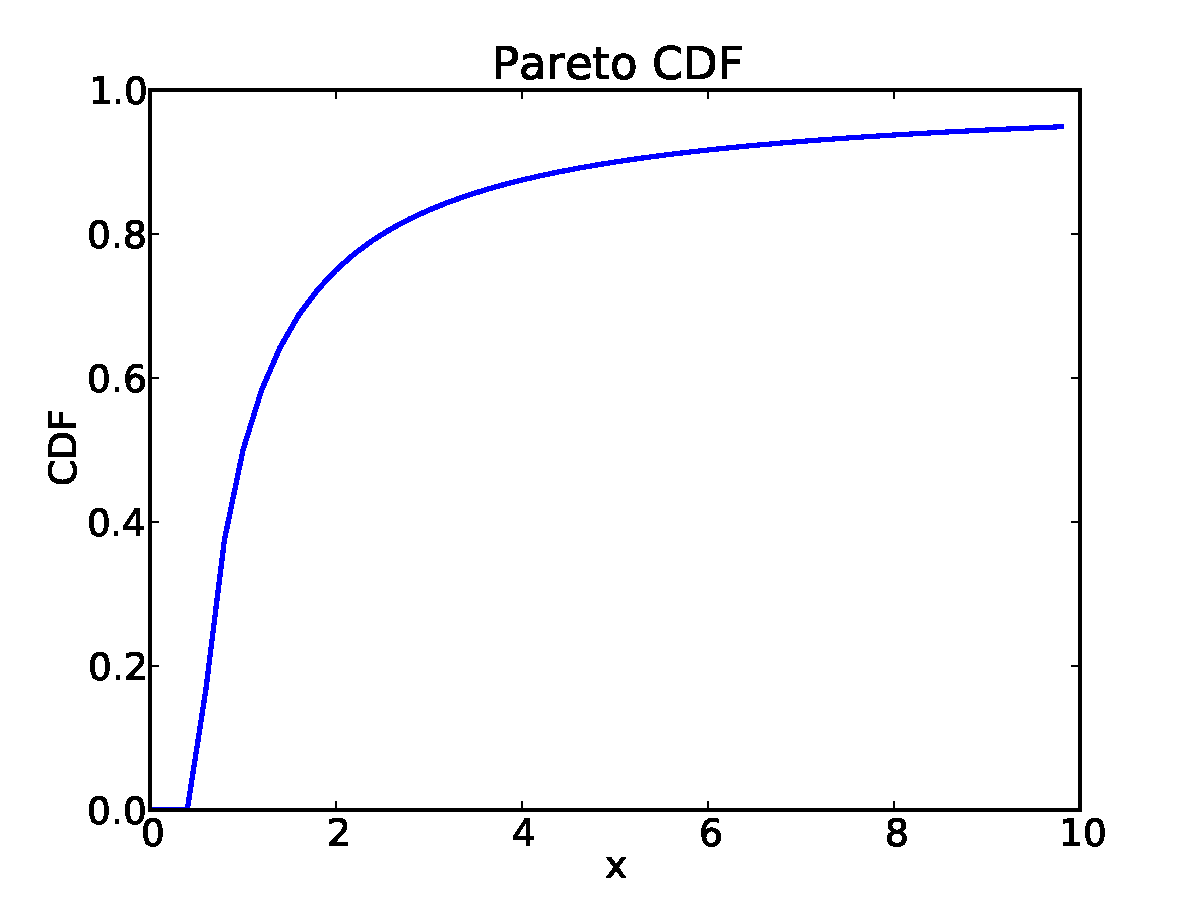
\includegraphics[height=2.5in]{figs/pareto_cdf.pdf}}
\caption{CDF of a Pareto distribution.}
\label{pareto_cdf}
\end{figure}

The median of this distribution is $x_m 2^{1/\alpha}$, which is 1, but
the 95th percentile is 10.  By contrast, the exponential distribution
with median 1 has 95th percentile of only 1.5.  \index{exponential
  distribution} \index{distribution!exponential} \index{median}
\index{logarithmic scale}

There is a simple visual test that indicates whether an empirical
distribution fits a Pareto distribution: on a log-log scale, the CCDF
looks like a straight line.
If you plot a the CCDF of a sample from a Pareto distribution on a
linear scale, you expect to see a function like:
%
\[ y \approx \left( \frac{x}{x_m} \right) ^{-\alpha} \]
%
Taking the log of both sides yields:

\Eqn{ log y \myapprox \minus\myalpha~(log \x~\minus~log x\sub{m}) }

So if you plot log \y~versus log \x, it should look like a straight
line with slope \minus\myalpha~and intercept
\myalpha~log \x\sub{m}.

\begin{exercise}
The {\tt random} module provides {\tt paretovariate},
which generates random values from a Pareto distribution.  It takes
a parameter for \myalpha, but not \x\sub{m}.  The
default value for \x\sub{m} is 1; you can generate a distribution
with a different parameter by multiplying by \x\sub{m}.
\index{random module}
\index{Pareto distribution}
\index{distribution!Pareto}

Write a wrapper function named {\tt paretovariate} that takes
\myalpha~and \x \sub{m} as parameters and uses {\tt
  random.paretovariate} to generate values from a two-parameter Pareto
distribution.
\index{parameter}

Use your function to generate a sample from a Pareto distribution.
Compute the CCDF and plot it on a log-log scale.  Is it a straight
line?  What is the slope?
\index{complementary CDF}
\index{CDF!complementary}
\index{CCDF}

\end{exercise}

\begin{exercise}
To get a feel for the Pareto distribution, imagine what the world
would be like if the distribution of human height were Pareto.
Choosing the parameters \x \sub{m}~=~100 cm and \myalpha~=~1.7, we
get a distribution with a reasonable minimum, 100 cm,
and median, 150 cm.
\index{height}

Generate 6 billion random values from this distribution.  What is the
mean of this sample?  What fraction of the population is shorter than
the mean?  How tall is the tallest person in Pareto World?
\index{Pareto World}

\end{exercise}

\begin{exercise}
Zipf's law is an observation about how often different words are used.
The most common words have very high frequencies, but there are many
unusual words, like ``hapaxlegomenon,'' that appear only a few times.
Zipf's law predicts that in a body of text, called a ``corpus,'' the
distribution of word frequencies is roughly Pareto.
\index{Pareto distribution}
\index{distribution!Pareto}
\index{Zipf's law}
\index{hapaxlegomenon}
\index{corpus}
\index{frequency}
\index{word frequency}

Find a large corpus, in any language, in electronic
format.  Count how many times each word appears.  Find the CCDF of the
word counts and plot it on a log-log scale.  Does Zipf's law hold?
What is the value of \myalpha, approximately?
\index{complementary CDF}
\index{CDF!complementary}
\index{CCDF}

\end{exercise}

\begin{exercise}
\label{weibull}

The Weibull distribution is a generalization of the exponential
distribution that comes up in failure analysis
(see \url{http://wikipedia.org/wiki/Weibull_distribution}).  Its CDF is
%
\[ CDF(x) = 1 - e^{-(x / \lambda)^k} \]
%
Can you find a transformation that makes a Weibull distribution look
like a straight line?  What do the slope and intercept of the
line indicate?
\index{Weibull distribution}
\index{distribution!Weibull}
\index{exponential distribution}
\index{distribution!exponential}
\index{random module}

Use {\tt random.weibullvariate} to generate a sample from a
Weibull distribution and use it to test your transformation.

\end{exercise}


\section{The normal distribution}
\label{normal}
\index{normal distribution}
\index{distribution!normal}
\index{Gaussian distribution}
\index{distribution!Gaussian}

\newcommand{\erf}{\mathrm{erf}}

The normal distribution, also called Gaussian, is the most commonly
used because it describes so many phenomena, at least approximately.
It turns out that there is a good reason for its ubiquity, which we
will get to in Section~\ref{CLT}.
\index{error function}
\index{CDF}

The normal distribution has many properties that make it amenable for
analysis, but the CDF is not one of them.  Unlike the
other distributions we have looked at, there is no closed-form
expression for the normal CDF; the most common alternative is to write
it in terms of the {\bf error function}, which is a special function
written erf(\x):
%
\[ CDF(x) = \frac{1}{2} \left[ 1 +
  \erf \left( \frac{x - \mu}{\sigma \sqrt{2}} \right) \right] \]
%
\[ \erf(x) = \frac{2}{\sqrt{\pi}} \int_{0}^x e^{-t^2} dt \]
%
The parameters \mymu~and \mysigma~determine the mean and standard
deviation of the distribution.
\index{parameter}
\index{{\tt erf.py}}

If these formulas make your eyes hurt, don't worry; they are easy to
implement in Python\footnote{As of Python 3.2, it is even easier; 
{\tt erf} is in the {\tt math} module.}.  There are many fast and
accurate ways to approximate erf(\x).  You can download one of them
from \url{http://thinkstats.com/erf.py}, which provides functions named
{\tt erf} and {\tt NormalCdf}.

Figure~\ref{normal_cdf} shows the CDF of the normal distribution
with parameters \mymu~=~2.0 and \mysigma~=~0.5.  The sigmoid shape of
this curve is a recognizable characteristic of a normal distribution.

\begin{figure}
% continuous.py
\centerline{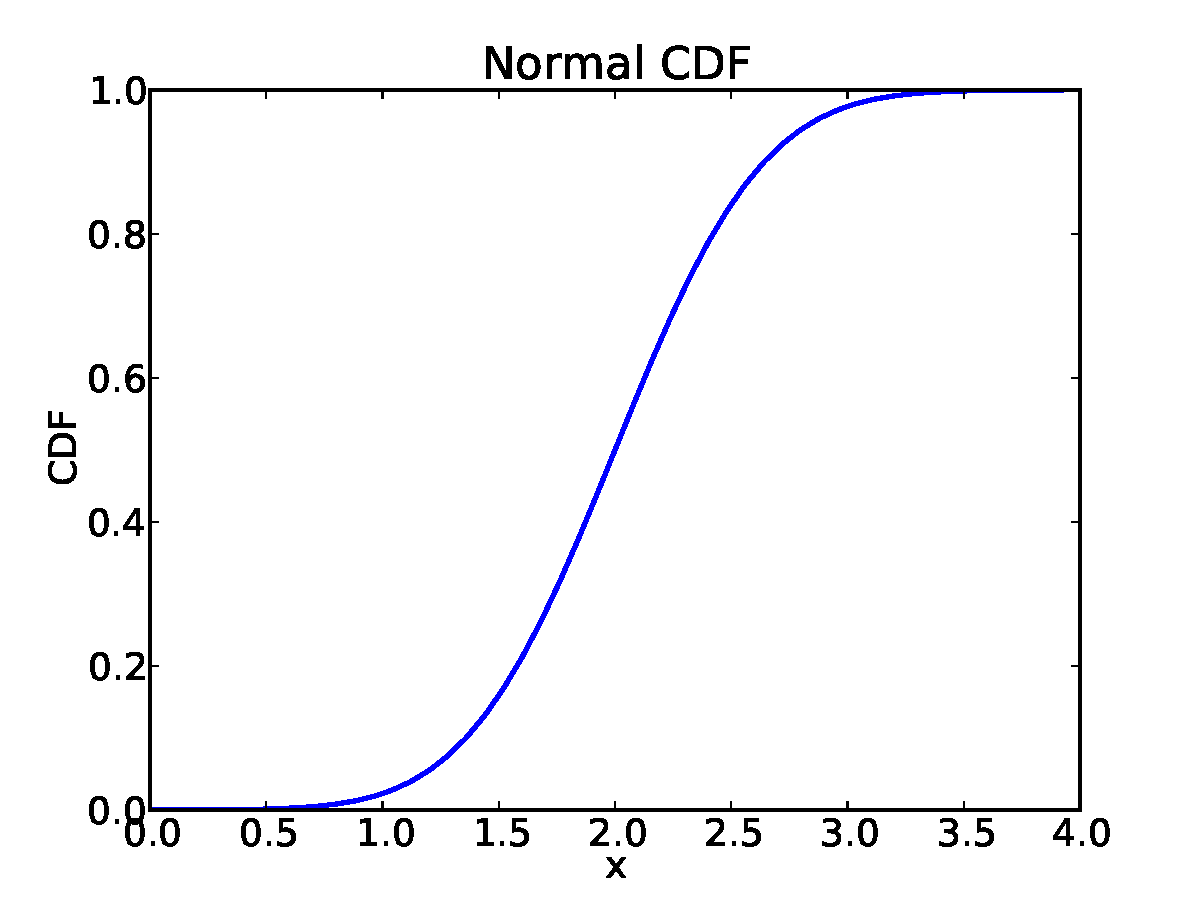
\includegraphics[height=2.5in]{figs/normal_cdf.pdf}}
\caption{CDF of a normal distribution.}
\label{normal_cdf}
\end{figure}

In the previous chapter we looked at the distribution of birth
weights in the NSFG.  Figure~\ref{nsfg_birthwgt_model} shows the
empirical CDF of weights for all live births and the CDF of
a normal distribution with the same mean and variance.
\index{National Survey of Family Growth}
\index{NSFG}
\index{birth weight}
\index{weight!birth}

\begin{figure}
% continuous.py
\centerline{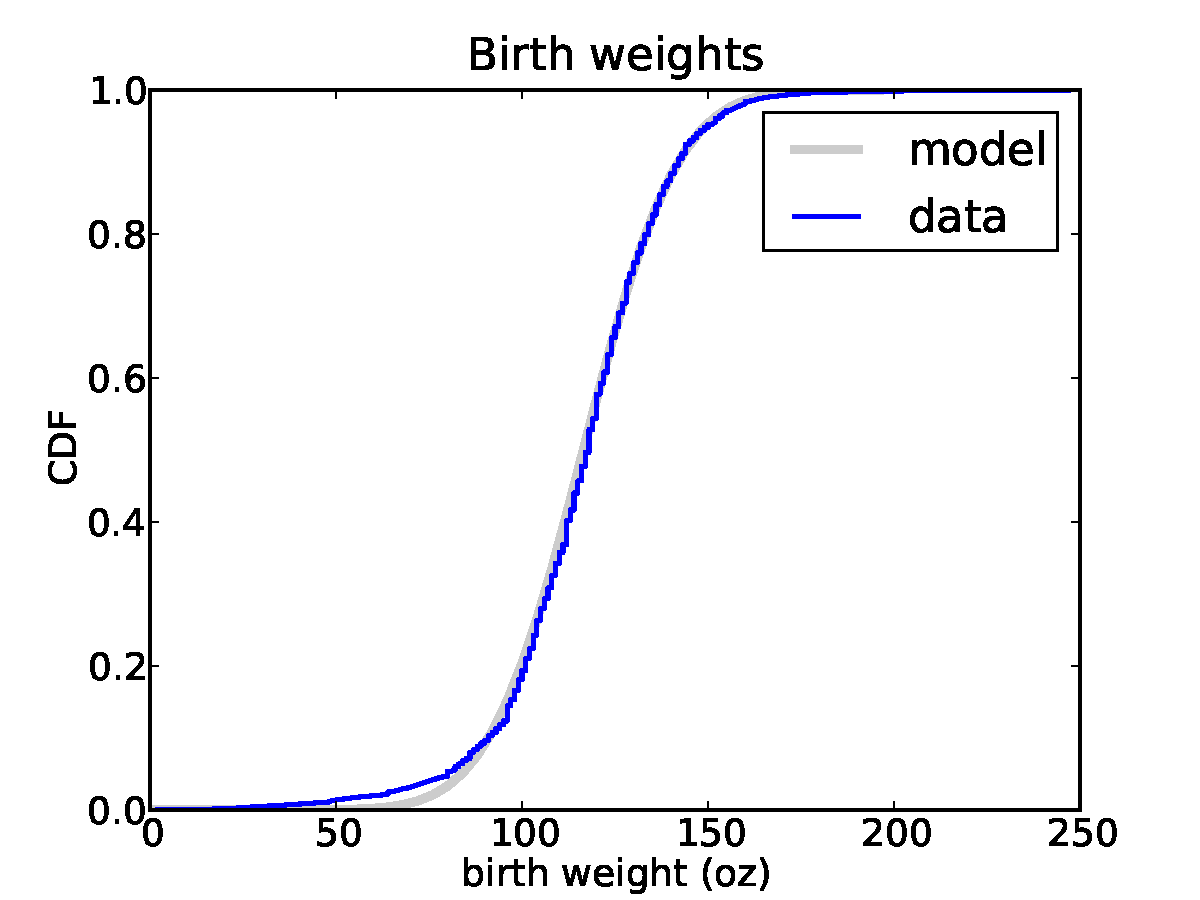
\includegraphics[height=2.5in]{figs/nsfg_birthwgt_model.pdf}}
\caption{CDF of birth weights with a normal model.}
\label{nsfg_birthwgt_model}
\end{figure}

The normal distribution is a good model for this dataset.  A {\bf
  model} is a useful simplification.  In this case it is useful
because we can summarize the entire distribution with just two
numbers, \mymu~=~116.5 and \mysigma~=~19.9, and the resulting error
(difference between the model and the data) is small.
\index{model}
\index{percentile}

Below the 10th percentile there is a discrepancy between the data
and the model; there are more light babies than we would expect in
a normal distribution.  If we are interested in studying preterm
babies, it would be important to get this part of the distribution
right, so it might not be appropriate to use the normal
model.

\begin{exercise}
The Wechsler Adult Intelligence Scale is a test that is intended
to measure intelligence\footnote{Whether it does or not is a
fascinating controversy that I invite you to investigate at your
leisure.}.  Results are transformed so that the distribution of scores
in the general population is normal with \mymu~=~100 and \mysigma~=~15.
\index{Wechsler Adult Intelligence Scale}
\index{Adult Intelligence Scale}
\index{WAIS}
\index{IQ}
\index{intelligence}

Use {\tt erf.NormalCdf} to investigate the frequency of rare events in
a normal distribution.  What fraction of the population has an IQ
greater than the mean?  What fraction is over 115?  130?  145?

A ``six-sigma'' event is a value that exceeds the mean by 6 standard
deviations, so a six-sigma IQ is 190.  In a world of 6 billion people,
how many do we expect to have an IQ of 190 or more\footnote{On this
  topic, you might be interested to read
  \url{http://wikipedia.org/wiki/Christopher_Langan}.}?
\index{Langan, Christopher}
\index{six-sigma event}

\end{exercise}


\begin{exercise}
Plot the CDF of pregnancy lengths for all live births.  Does it
look like a normal distribution?
\index{pregnancy length}
\index{length!pregnancy}

Compute the mean and variance of the sample and plot the normal
distribution with the same parameters.  Is the normal distribution a
good model for this data?  If you had to summarize this distribution
with two statistics, what statistics would you choose?

\end{exercise}


\section{Normal probability plot}
\index{normal probability plot}
\index{plot!normal probability}
\index{exponential distribution}
\index{distribution!exponential}
\index{Weibull distribution}
\index{distribution!Weibull}
\index{Pareto distribution}
\index{distribution!Pareto}

For the exponential, Pareto and Weibull distributions, there are
simple transformations we can use to test whether a continuous
distribution is a good model of a dataset.
\index{model}
\index{normal distribution}
\index{distribution!normal}
\index{Gaussian distribution}
\index{distribution!Gaussian}

For the normal distribution there is no such transformation, but there
is an alternative called a {\bf normal probability plot}.  It is based
on {\bf rankits}: if you generate \n~values from a normal
distribution and sort them, the \kk th rankit is the mean of the
distribution for the \kk th value.
\index{rankit}

\begin{exercise}
Write a function called {\tt Sample} that generates 6 samples from a
normal distribution with \mymu~=~0 and \mysigma~=~1.  Sort and return
the values.

Write a function called {\tt Samples} that calls {\tt Sample} 1000 times and
returns a list of 1000 lists.

If you apply {\tt zip} to this list of lists, the result is 6 lists
with 1000 values in each.  Compute the mean of each of these lists
and print the results.  I predict that you will get something like
this:

\{\minus1.2672,   \minus0.6418,   \minus0.2016,   0.2016,   0.6418,   1.2672\}

If you increase the number of times you call {\tt Sample}, the
results should converge on these values.

\end{exercise}

% Algorithms for exact and approximate normal rank stats
% http://download.osgeo.org/grass/grass6_progman/as177_8c_source.html

Computing rankits exactly is moderately difficult, but there are
numerical methods for approximating them.  And there is a
quick-and-dirty method that is even easier to implement:

\begin{enumerate}

\item From a normal distribution with \mymu~=~0 and \mysigma~=~1,
generate a sample with the same size as your dataset and sort it.

\item Sort the values in the dataset.

\item Plot the sorted values from your dataset versus the random values.

\end{enumerate}

For large datasets, this method works well.
For smaller datasets, you can improve it by generating \m (\n+1)~\minus~1
values from a normal distribution, where \n~is the size of the
dataset and \m~is a multiplier.  Then select every \m th element,
starting with the \m th.  

%Hint: use the Python slice operator.

This method works with other distributions as well, as long as
you know how to generate a random sample.

Figure~\ref{nsfg_birthwgt_normal} is a quick-and-dirty normal
probability plot for the birth weight data.
\index{birth weight}
\index{weight!birth}

\begin{figure}
% continuous.py
\centerline{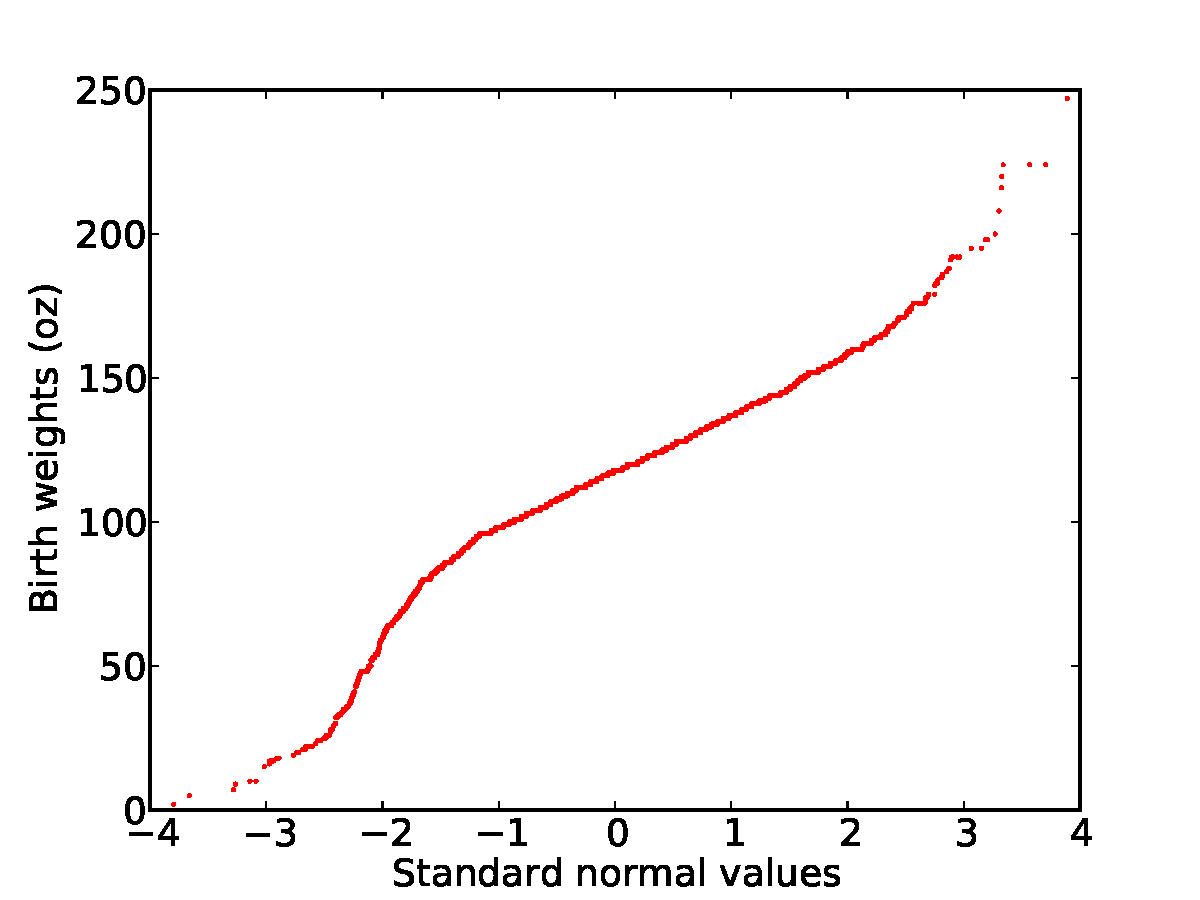
\includegraphics[height=2.5in]{figs/nsfg_birthwgt_normal.pdf}}
\caption{Normal probability plot of birth weights.}
\label{nsfg_birthwgt_normal}
\end{figure}

The curvature in this plot suggests that there are
deviations from a normal distribution; nevertheless, it is a
good (enough) model for many purposes.
\index{model}

\begin{exercise}
Write a function called {\tt NormalPlot} that takes a sequence of
values and generates a normal probability plot.  You can download
a solution from \url{http://thinkstats.com/rankit.py}.
\index{normal distribution}
\index{distribution!normal}
\index{Gaussian distribution}
\index{distribution!Gaussian}
\index{{\tt rankit.py}}
\index{{\tt relay.py}}
\index{{\tt relay\_normal.py}}
\index{relay race}
\index{race!relay}

Use the running speeds from {\tt relay.py} to generate a normal
probability plot.  Is the normal distribution a good model for this
data?  You can download a solution from
\url{http://thinkstats.com/relay_normal.py}.

\end{exercise}


\section{The lognormal distribution}
\label{lognormal}
\index{lognormal distribution}
\index{distribution!lognormal}
\index{CDF}

If the logarithms of a set of values have a normal distribution, the
values have a {\bf lognormal} distribution.  The CDF of the lognormal
distribution is the same as the CDF of the normal distribution,
with log \x~substituted for \x.

\Eqn{ CDF\sub{lognormal}(\x) = CDF\sub{normal}(log \x) }
 
The parameters of the lognormal distribution are usually denoted
\mymu~and \mysigma.  But remember that these parameters are {\em not}
the mean and standard deviation; the mean of a lognormal distribution
is exp(\mymu~+~\sigmasq/2) and the standard deviation is
ugly\footnote{See \url{http://wikipedia.org/wiki/Log-normal_distribution}.}.
\index{parameter} \index{weight!adult} \index{adult weight}

It turns out that the distribution of weights for adults is
approximately lognormal\footnote{I was tipped off to this possibility by a
  comment (without citation) at
  \url{http://mathworld.wolfram.com/LogNormalDistribution.html}.
  Subsequently I found a paper that proposes the log transform and
  suggests a cause: Penman and Johnson, ``The Changing Shape of the
  Body Mass Index Distribution Curve in the Population,'' Preventing
  Chronic Disease, 2006 July; 3(3): A74.  Online
  at \url{http://www.ncbi.nlm.nih.gov/pmc/articles/PMC1636707}.}.

The National Center for Chronic Disease
Prevention and Health Promotion conducts an annual survey as part of
the Behavioral Risk Factor Surveillance System
(BRFSS)\footnote{Centers for Disease Control and Prevention
  (CDC). Behavioral Risk Factor Surveillance System Survey
  Data. Atlanta, Georgia: U.S. Department of Health and Human
  Services, Centers for Disease Control and Prevention, 2008.}.  In
2008, they interviewed 414,509 respondents and asked about their
demographics, health and health risks.
\index{Behavioral Risk Factor Surveillance System}
\index{BRFSS}


\begin{figure}
% cumulative.py
\centerline{
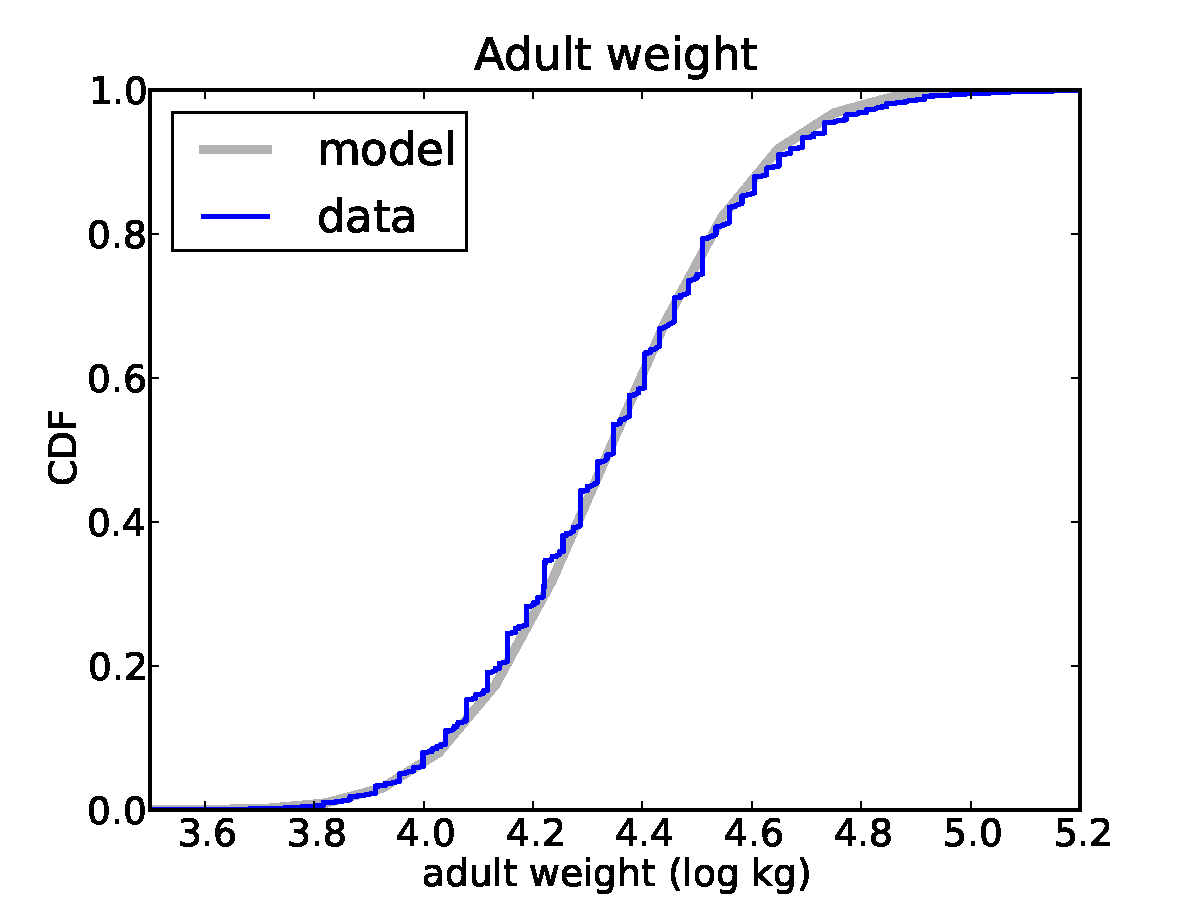
\includegraphics[height=2.5in]{figs/brfss_weight_log.pdf}
}
\caption{CDF of adult weights (log
  transform).}
\label{brfss_weight_log}
\end{figure}

Among the data they collected are the weights in kilograms of
398,484 respondents.
Figure~\ref{brfss_weight_log} shows the distribution
of log \w, where \w~is weight in kilograms, along with a normal
model.
\index{respondent}
\index{model}

The normal model is a good fit for the data, although the highest
weights exceed what we expect from the normal model even after the log
transform.  Since the distribution of log \w~fits a normal distribution, we
conclude that \w~fits a lognormal distribution.
\index{normal distribution}
\index{distribution!normal}
\index{Gaussian distribution}
\index{distribution!Gaussian}
\index{lognormal distribution}
\index{distribution!lognormal}


%Figure~\ref{brfss_weight_model} shows the
%distribution of these weights and a normal model with the same mean
%and variance.

%\begin{figure}
%\centerline{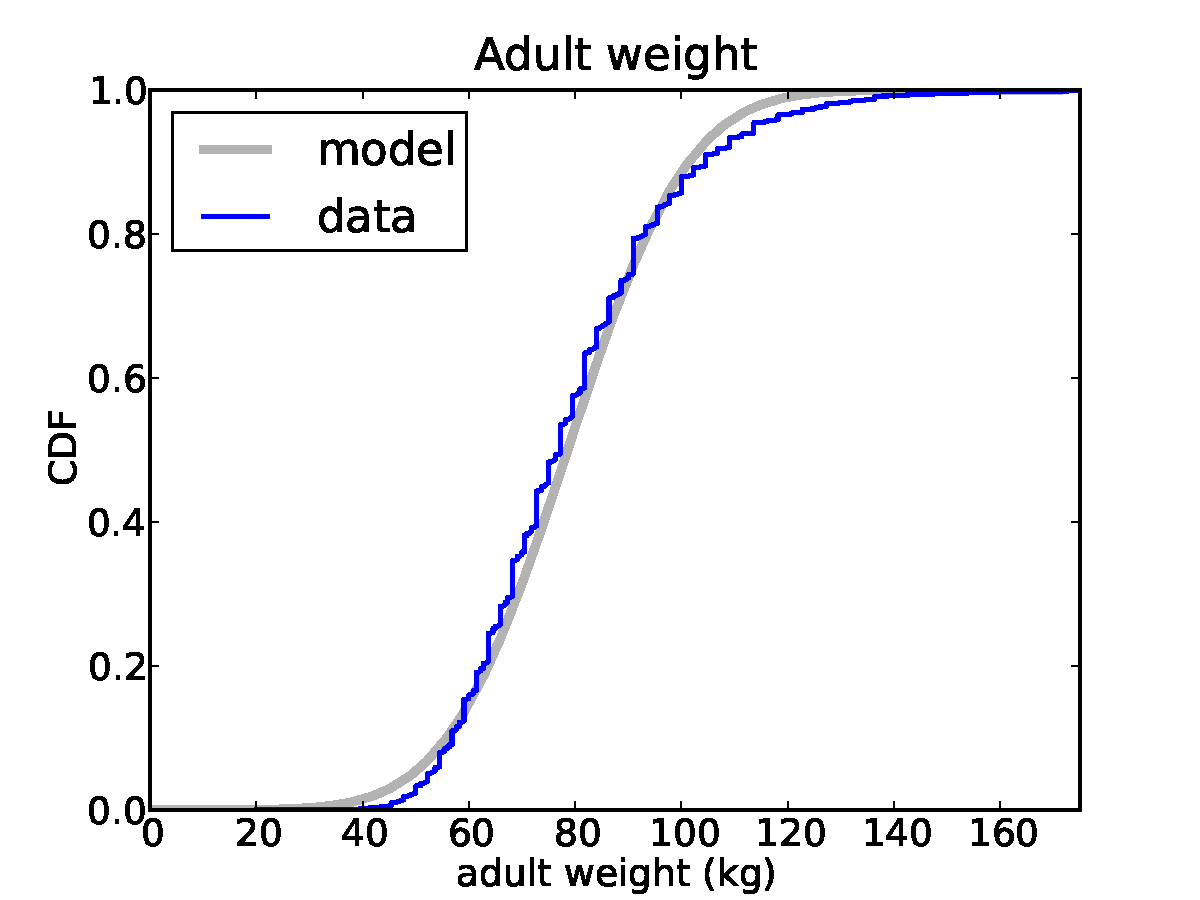
\includegraphics[height=2.5in]{figs/brfss_weight_model.pdf}}
%\caption{CDF of adult weights from the BRFSS.}
%\label{brfss_weight_model}
%\end{figure}

%The agreement between the data and the model might be good enough
%for some purposes, but there are clear discrepancies below the 10th
%and above the 90th percentile.

%\begin{figure}
%\centerline{
%\begin{tabular}{cc}
%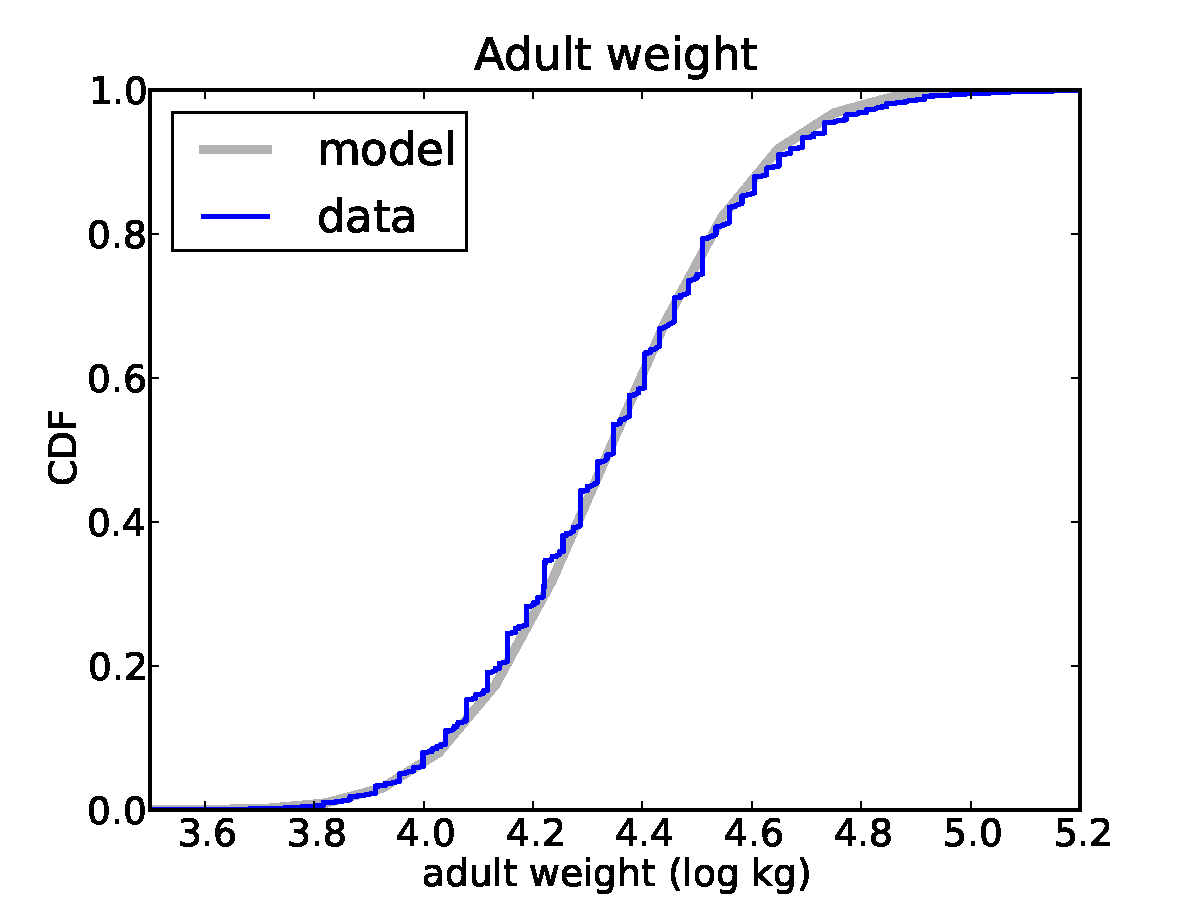
\includegraphics[height=2.3in]{figs/brfss_weight_log.pdf}
%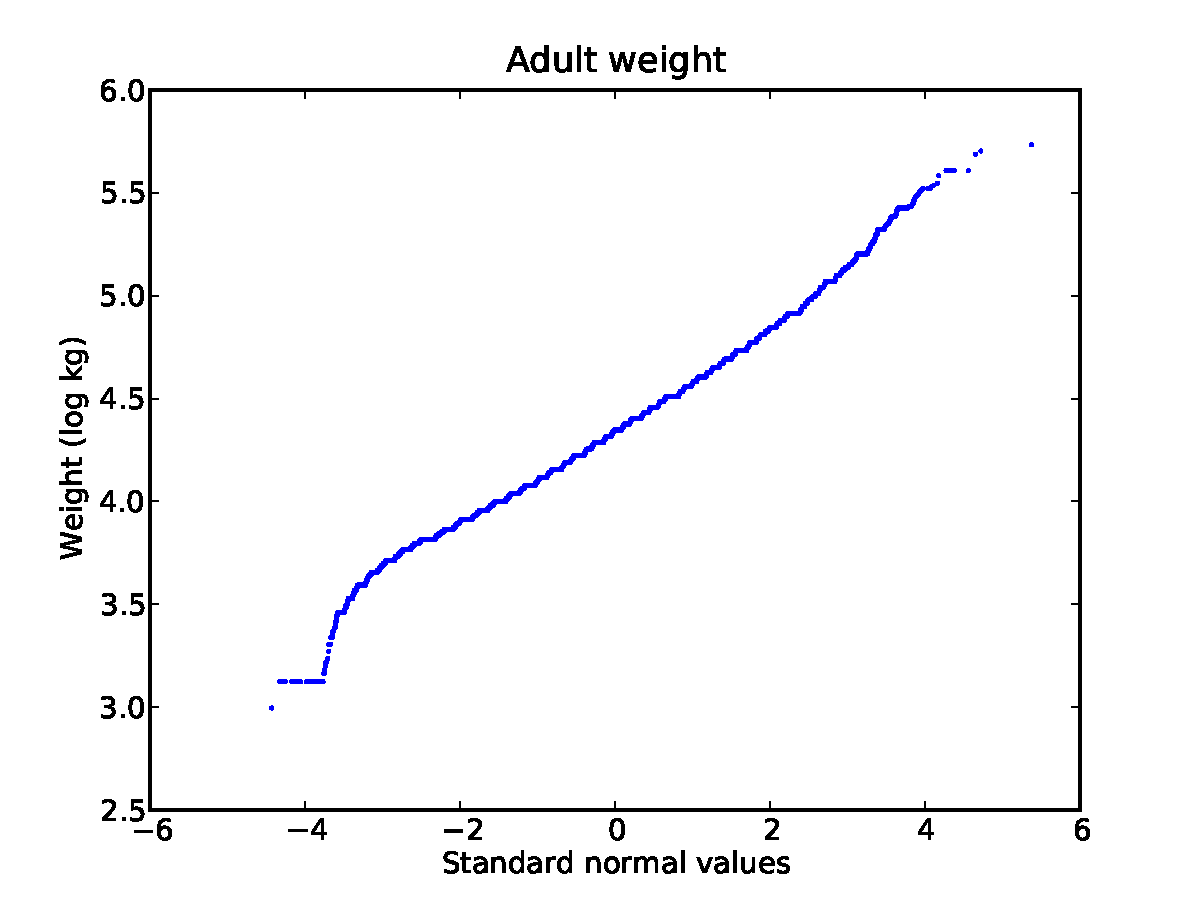
\includegraphics[height=2.3in]{figs/brfss_weight_lognormal.pdf}
%\end{tabular}
%}
%\caption{CDF and normal probability plot for adult weights (log
%  transform).}
%\label{brfss_weight_log}
%\end{figure}

\begin{exercise}
Download the BRFSS data from 
\url{http://thinkstats.com/CDBRFS08.ASC.gz}, and my code for reading it
from
\url{http://thinkstats.com/brfss.py}.  Run {\tt brfss.py} and confirm that
it prints summary statistics for a few of the variables.
\index{Behavioral Risk Factor Surveillance System}
\index{BRFSS}
\index{{\tt brfss.py}}
\index{{\tt brfss\_figs.py}}
\index{weight!adult}
\index{adult weight}

Write a program that reads adult weights from the BRFSS and
generates normal probability plots for \w~and log \w.  You can
download a solution from \url{http://thinkstats.com/brfss_figs.py}.

\end{exercise}

\begin{exercise}
The distribution of populations for cities and towns has been proposed
as an example of a real-world phenomenon that can be described
with a Pareto distribution.
\index{Pareto distribution}
\index{distribution!Pareto}
\index{U.S.~Census Bureau}
\index{population}
\index{city size}

The U.S.~Census Bureau publishes data on the population of every
incorporated city and town in the United States.  I have written a
small program that downloads this data and stores it in a file.  You
can download it from \url{http://thinkstats.com/populations.py}.
\index{{\tt populations.py}}

\begin{enumerate}

\item Read over the program to make sure you know what it does; then
  run it to download and process the data.

\item Write a program that computes and plots the distribution of
  populations for the 14,593 cities and towns in the dataset.

\item Plot the CDF on linear and log-\x~scales so you can get a sense
  of the shape of the distribution.  Then plot the CCDF on a log-log
  scale to see if it has the characteristic shape of a Pareto
  distribution.
\index{complementary CDF}
\index{CDF!complementary}
\index{CCDF}

\item Try out the other transformations and plots in this chapter to
  see if there is a better model for this data.

\end{enumerate}

What conclusion do you draw about the distribution of sizes
for cities and towns?  You can download a solution from
\url{http://thinkstats.com/populations_cdf.py}.
\index{{\tt populations\_cdf.py}}

\end{exercise}


\begin{exercise}
\label{irs}

The Internal Revenue Service of the United States (IRS) provides data
about income taxes at \url{http://irs.gov/taxstats}.
\index{Internal Revenue Service}
\index{IRS}
\index{income}
\index{taxes}

One of their files, containing information about individual incomes
for 2008, is available from \url{http://thinkstats.com/08in11si.csv}.  I
converted it to a text format called CSV, which stands for
``comma-separated values;'' you can read it using the {\tt csv}
module.

Extract the distribution of incomes from this dataset.  Are any of
the continuous distributions in this chapter a good model of
the data?  You can download a solution from \url{http://thinkstats.com/irs.py}.
\index{{\tt irs.py}}

\end{exercise}


\section{Why model?}
\index{model}

At the beginning of this chapter I said that many real world phenomena
can be modeled with continuous distributions.  ``So,'' you might ask,
``what?''
\index{abstraction}

Like all models, continuous distributions are abstractions, which
means they leave out details that are considered irrelevant.
For example, an observed distribution might have measurement errors
or quirks that are specific to the sample; continuous models smooth
out these idiosyncrasies.
\index{smoothing}

Continuous models are also a form of data compression.  When a model
fits a dataset well, a small set of parameters can summarize a
large amount of data.
\index{parameter}
\index{compression}

It is sometimes surprising when data from a natural phenomenon fit a
continuous distribution, but these observations can lead to insight
into physical systems.  Sometimes we can explain why an observed
distribution has a particular form.  For example, Pareto distributions
are often the result of generative processes with positive feedback
(so-called preferential attachment processes: see
\url{http://wikipedia.org/wiki/Preferential_attachment}.).
\index{preferential attachment}
\index{generative process}
\index{Pareto distribution}
\index{distribution!Pareto}
\index{analysis}

Continuous distributions lend themselves to mathematical analysis, as
we will see in Chapter~\ref{operations}.


\section{Generating random numbers}
\index{exponential distribution}
\index{distribution!exponential}
\index{random number}
\index{CDF}
\index{inverse CDF algorithm}
\index{uniform distribution}
\index{distribution!uniform}

Continuous CDFs are also useful for generating random numbers.
If there is an efficient way to compute the inverse CDF, ICDF(\p),
we can generate random values with the appropriate distribution
by choosing from a uniform distribution from 0 to 1, then choosing

\Eqn{ \x~=~ICDF(\p) }

For example, the CDF of the exponential distribution is
%
\[ p = 1 - e^{-\lambda x} \]
%
Solving for \x~yields:

\Eqn{ \x = \minus log (1~\minus~\p) / \mylambda }

So in Python we can write
%
\begin{verbatim}
def expovariate(lam):
    p = random.random()
    x = -math.log(1-p) / lam
    return x
\end{verbatim}

I called the parameter \verb"lam" because \verb"lambda" is a Python
keyword.  Most implementations of {\tt random.random} can return 0 but
not 1, so 1~\minus~\p~can be 1 but not 0, which is good, because log 0 is
undefined.
\index{random module}

\begin{exercise}
Write a function named \verb"weibullvariate" that takes
\verb"lam" and \verb"k" and returns a random value from the Weibull
distribution with those parameters.
\index{Weibull distribution}
\index{distribution!Weibull}
\index{parameter}

\end{exercise}


\section{Glossary}

\begin{description}

\item[empirical distribution:] The distribution of values in a sample.
\index{empirical distribution}
\index{distribution!empirical}

\item[continuous distribution:] A distribution described by a continuous
function.
\index{continuous distribution}
\index{distribution!continuous}

\item[interarrival time:] The elapsed time between two events.
\index{interarrival time}

\item[error function:] A special mathematical function, so-named
  because it comes up in the study of measurement errors.
\index{error function}

\item[normal probability plot:] A plot of the sorted values in a sample
versus the expected value for each if their distribution is normal.
\index{normal probability plot}
\index{plot!normal probability}

\item[rankit:] The expected value of an element in a sorted list of
values from a normal distribution.
\index{rankit}

\item[model:] A useful simplification.  Continuous distributions are
often good models of more complex empirical distributions.
\index{model}

\item[corpus:] A body of text used as a sample of a language.
\index{corpus}

\item[hapaxlegomenon:] A word that appears only once in a corpus.
It appears twice in this book, so far.
\index{hapaxlegomenon}

\end{description}


\chapter{Probability}
\label{probability}
\index{probability}
\index{frequency}
\index{sample size}

In Chapter~\ref{descriptive}, I said that a probability is a frequency
expressed as a fraction of the sample size.  That's one definition of
probability, but it's not the only one.  In fact, the meaning
of probability is a topic of some controversy.

We'll start with the uncontroversial parts and work our way up.  There
is general agreement that a probability is a real value between 0 and
1 that is intended to be a quantitative measure corresponding to the
qualitative notion that some things are more likely than others.
\index{event}
\index{trial}

The ``things'' we assign probabilities to are called {\bf events}.  If
\E~represents an event, then \Prob(\E) represents the probability that
\E~will occur.  A situation where \E~might or might not happen is
called a {\bf trial}.
\index{success}
\index{failure}
\index{dice}

As an example, suppose you have a standard six-sided
die\footnote{``Die'' is the singular of ``dice''.} and want to know
the probability of rolling a 6.  Each roll is a trial.
Each time a 6 appears is considered a {\bf success}; other trials are
considered {\bf failures}.  These terms are used even in scenarios
where ``success'' is bad and ``failure'' is good.

If we have a finite sample of \n~trials and we observe \s~successes,
the probability of success is \s/\n.  If the set of trials is
infinite, defining probabilities is a little trickier, but most people
are willing to accept probabilistic claims about a hypothetical series
of identical trials, like tossing a coin or rolling a die.
\index{identical trials}
\index{unique events}

We start to run into trouble when we talk about probabilities of
unique events.  For example, we might like to know the probability
that a candidate will win an election.  But every election is unique,
so there is no series of identical trials to consider.
\index{election}

In cases like this some people would say that the notion of
probability does not apply.  This position is sometimes called {\bf
  frequentism} because it defines probability in terms of frequencies.
If there is no set of identical trials, there is no probability.
\index{frequentism}
\index{Bayesianism}

Frequentism is philosophically safe, but
frustrating because it limits the scope of probability to physical
systems that are either random (like atomic decay) or so unpredictable
that we model them as random (like a tumbling die).  Anything involving
people is pretty much off the table.

An alternative is {\bf Bayesianism}, which defines probability as
a degree of belief that an event will occur.  By this definition,
the notion of probability can be applied in almost any circumstance.
One difficulty with Bayesian probability is that it depends on
a person's state of knowledge; people with different information
might have different degrees of belief about the same event.  For
this reason, many people think that Bayesian probabilities are
more subjective than frequency probabilities.
\index{subjective belief}
\index{belief}
\index{Thaksin Shinawatra}
\index{Thailand}
\index{Prime Minister}

As an example, what is the probability that Thaksin Shinawatra is the
Prime Minister of Thailand?  A frequentist would say that there is no
probability for this event because there is no set of
trials.  Thaksin either is, or is not, the PM; it's not a question of
probability.

In contrast, a Bayesian would be willing to assign a probability to
this event based on his or her state of knowledge.  For example, if
you remember that there was a coup in Thailand in 2006, and you are
pretty sure Thaksin was the PM who was ousted, you might
assign a probability like 0.1, which acknowledges the possibility
that your recollection is incorrect, or that Thaksin has been
reinstated.

If you consult Wikipedia, you will learn that Thaksin is not the
PM of Thailand (at the time I am writing).  Based on this
information, you might revise your probability estimate to 0.01,
reflecting the possibility that Wikipedia is wrong.


\section{Rules of probability}
\index{probability!rules of}

\newcommand{\AND}{~\mbox{and}~}

For frequency probabilities, we can derive rules that relate
probabilities of different events.  Probably the best known of these
rules is

\Eqn{ \Prob(\A \AND \B) = \Prob(\A) \Prob(\B) \quad Warning: not always true! }

where \Prob(\A \AND \B) is the probability that events \A~and \B~both
occur.  This formula is easy to remember; the only problem is that it
is {\em not always true}.  This formula only applies if \A~and \B~are 
{\bf independent}, which means that if I know \A~occurred, that
doesn't change the probability of \B, and vice versa.
\index{independent}
\index{event!independent}

For example, if \A~is tossing a coin and getting heads, and \B~is 
rolling a die and getting 1, \A~and \B~are independent, because
the coin toss doesn't tell me anything about the die roll.
\index{dice}

But if I roll two dice, and \A~is getting at least one six, and
\B~is getting two sixes, \A~and \B~are not independent, because
if I know that \A~occurred, the probability of \B~is higher, and
if I know \B~occurred, the probability of \A~is 1.
\index{conditional probability}
\index{probability!conditional}

When \A~and \B~are not independent, it is often useful to compute
the conditional probability, \Prob(\A|\B), which is the probability of
\A~given that we know \B~occurred:
%
\[ P(A|B) = \frac{P(A \AND B)}{P(B)} \]
%
From that we can derive the general relation

\Eqn{ \Prob(\A \AND \B) = \Prob(\A) \Prob(\B|\A) }

This might not be as easy to remember, but if you translate it into
English it should make sense: ``The chance of both things happening
is the chance that the first one happens, and then the second one
given the first.''

There is nothing special about the order of events, so we could also
write

\Eqn{ \Prob(\A \AND \B) = \Prob(\B) \Prob(\A|\B) }

These relationships hold whether \A~and \B~are independent or not.
If they are independent, then \Prob(\A|\B)~=~\Prob(\A), which gets us back
where we started.

Because all probabilities are in the range 0 to 1, it is
easy to show that 

\Eqn{ \Prob(\A \AND \B)~\myle~\Prob(\A) }

To picture this, imagine a club that only admits people who satisfy
some requirement, \A.  Now suppose they add a new requirement for
membership, \B.  It seems obvious that the club will get smaller, or
stay the same if it happens that all the members satisfy \B.  But
there are some scenarios where people are surprisingly bad at this
kind of analysis.  For examples and discussion of this phenomenon, see
\url{http://wikipedia.org/wiki/Conjunction_fallacy}.
\index{conjunction fallacy}
\index{fallacy!conjunction}

\begin{exercise}
If I roll two dice and the total is 8, what is the chance that
one of the dice is a 6?
\index{dice}

\end{exercise}

\begin{exercise}
If I roll 100 dice, what is the chance of getting all sixes?
What is the chance of getting no sixes?

\end{exercise}

\begin{exercise}
The following questions are adapted from Mlodinow, {\em The Drunkard's
  Walk}.
\index{Mlodinow, Leonard}
\index{Florida, girl named}
\index{girl named Florida}

\begin{enumerate}

\item If a family has two children, what is the chance that they
  have two girls?

\item If a family has two children and we know that at least one of
  them is a girl, what is the chance that they have two girls?

\item If a family has two children and we know that the older one is a
  girl, what is the chance that they have two girls?

\item If a family has two children and we know that at least one of
  them is a girl named Florida, what is the chance that they have
  two girls?

\end{enumerate}

You can assume that the probability that any child is a girl is 1/2,
and that the children in a family are independent trials (in more ways
than one).  You can also assume that the percentage of girls named
Florida is small.

\end{exercise}


\section{Monty Hall}
\index{Monty Hall problem}

The Monty Hall problem might be the most contentious question in
the history of probability.  The scenario is simple, but the correct
answer is so counter-intuitive that many people just can't accept
it, and many smart people have embarrassed themselves not just by
getting it wrong but by arguing the wrong side, aggressively,
in public.

Monty Hall was the original host of the game show {\em Let's Make a
Deal}.  The Monty Hall problem is based on one of the regular
games on the show.  If you are on the show, here's what happens:

\begin{itemize}

\item Monty shows you three closed doors and tells you that there is a
  prize behind each door: one prize is a car, the other two are less
  valuable prizes like peanut butter and fake finger nails.  The
  prizes are arranged at random.

\item The object of the game is to guess which door has the car.  If
  you guess right, you get to keep the car.

\item So you pick a door, which we will call Door A.  We'll call the
  other doors B and C.

\item Before opening the door you chose, Monty likes to increase the
  suspense by opening either Door B or C, whichever does not
  have the car.  (If the car is actually behind Door A, Monty can
  safely open B or C, so he chooses one at random).

\item Then Monty offers you the option to stick with your original
  choice or switch to the one remaining unopened door.

\end{itemize}

The question is, should you ``stick'' or ``switch'' or does it
make no difference?
\index{stick}
\index{switch}
\index{intuition}

Most people have the strong intuition that it makes no difference.
There are two doors left, they reason, so the chance that the car
is behind Door A is 50\%.

But that is wrong.  In fact, the chance of winning if you stick
with Door A is only 1/3; if you switch, your chances are 2/3.
I will explain why, but I don't expect you to believe me.

The key is to realize that there are three possible scenarios:
the car is behind Door A, B or C.  Since the prizes are
arranged at random, the probability of each scenario is 1/3.

If your strategy is to stick with Door A, then you will
win only in Scenario A, which has probability 1/3.

If your strategy is to switch, you will win in either Scenario
B or Scenario C, so the total probability of winning is 2/3.

%\index{\Erdos, Paul}

If you are not completely convinced by this argument, you are
in good company.  When a friend presented this solution to
Paul \Erdos, he replied, ``No, that is impossible.  It should
make no difference.\footnote{See Hoffman, {\em The Man Who Loved
Only Numbers}, page 83.}''

No amount of argument could convince him.  In the end, it took
a computer simulation to bring him around.

\begin{exercise}
Write a program that simulates the Monty Hall problem and use
it to estimate the probability of winning if you stick and if
you switch.

Then read the discussion of the problem at
\url{http://wikipedia.org/wiki/Monty_Hall_problem}.

Which do you find more convincing, the simulation or the arguments,
and why?

\end{exercise}


\begin{exercise}
To understand the Monty Hall problem, it is important to realize
that by deciding which door to open, Monty is giving you information.
To see why this matters, imagine the case where Monty doesn't
know where the prizes are, so he chooses Door B or C at random.
\index{Monty Hall! confused}
\index{confused Monty problem}

If he opens the door with the car, the game is over, you lose, and
you don't get to choose whether to switch or stick.

Otherwise, are you better off switching or sticking?

\end{exercise}



\newcommand{\Poincare}{Poincar\'{e}}

\section{\Poincare}
%\index{\Poincare, Henry}

Henri \Poincare~was a French mathematician who taught at the Sorbonne
around 1900.  The following anecdote about him is probably fabricated,
but it makes an interesting probability problem.
\index{bread police}

Supposedly \Poincare~suspected that his local bakery was selling
loaves of bread that were lighter than the advertised weight of 1 kg,
so every day for a year he bought a loaf of bread, brought it home and
weighed it.  At the end of the year, he plotted the distribution of
his measurements and showed that it fit a normal distribution with
mean 950 g and standard deviation 50 g.  He brought this evidence to
the bread police, who gave the baker a warning.
\index{normal distribution}
\index{distribution!normal}
\index{Gaussian distribution}
\index{distribution!Gaussian}

For the next year, \Poincare~continued the practice of weighing his
bread every day.  At the end of the year, he found that the average
weight was 1000 g, just as it should be, but again he complained to
the bread police, and this time they fined the baker.
\index{symmetric}

Why?  Because the shape of the distribution was asymmetric.  Unlike
the normal distribution, it was skewed to the right, which is
consistent with the hypothesis that the baker was still making 950 g
loaves, but deliberately giving \Poincare~the heavier ones.


\begin{exercise}
Write a program that simulates a baker who chooses \n~loaves from a
distribution with mean 950 g and standard deviation 50 g, and gives
the heaviest one to \Poincare.  What value of \n~yields a
distribution with mean 1000 g?  What is the standard deviation?

Compare this distribution to a normal distribution with the same mean
and the same standard deviation.  Is the difference in the shape of
the distribution big enough to convince the bread police?

\end{exercise}


\begin{exercise}
\label{coef_var}
If you go to a dance where partners are paired up randomly, what
percentage of opposite sex couples will you see where the woman is
taller than the man?
\index{dance}
\index{height}
\index{Behavioral Risk Factor Surveillance System}
\index{BRFSS}

In the BRFSS (see Section~\ref{lognormal}), the distribution of
heights is roughly normal with parameters \mymu~=~178 cm and
\sigmasq~=~59.4 cm for men, and \mymu~=~163 cm and \sigmasq~=~52.8 cm for
women.
\index{lognormal distribution}
\index{distribution!lognormal}


As an aside, you might notice that the standard deviation for men is
higher and wonder whether men's heights are more variable.  To compare
variability between groups, it is useful to compute the {\bf
  coefficient of variation}, which is the standard deviation as a
fraction of the mean, \mysigma/\mymu.  By this measure, women's
heights are slightly more variable.
\index{coefficient!variation}

% From brfss.py
%    mean          var           std           cv
% 1 178.090966766 59.4275328443 7.70892553112 0.0432864488925
% 2 163.226104443 52.7684723388 7.26419110011 0.0445038563217

\end{exercise}

\section{Another rule of probability}
\index{probability!rules of}
\index{mutually exclusive}

\newcommand{\OR}{~\mbox{or}~}
\newcommand{\NOT}{~\mbox{not}~}

If two events are {\bf mutually exclusive}, that means that only
one of them can happen, so the conditional probabilities are 0:

\Eqn{ \Prob(\A|\B) = \Prob(\B|\A) = 0 }

In this case it is easy to compute the probability of either event:

\Eqn{ \Prob(\A \OR \B) = \Prob(\A)~+~\Prob(\B) \quad Warning: not always true.}

But remember that this only applies if the events are mutually
exclusive.  In general the probability of \A~or \B~or both is:

\Eqn{ \Prob(\A \OR \B) = \Prob(\A)~+~\Prob(\B)~\minus~\Prob(\A \AND \B) }

The reason we have to subtract off \Prob(\A \AND \B) is that otherwise it
gets counted twice.  For example, if I flip two coins, the chance of
getting at least one tails is 1/2~+~1/2~\minus~1/4.  I have to subtract
1/4 because otherwise I am counting heads-heads twice.  The problem
becomes even clearer if I toss three coins.
\index{coin}

\begin{exercise}
If I roll two dice, what is the chance of rolling at least one 6?
\index{dice}

% 1/6 + 1/6 - 1/36

\end{exercise}

\begin{exercise}
What is the general formula for the probability of \A~or \B~but not both?

% P(A XOR B) = P(A) + P(B) - 2 P(A \AND B)

\end{exercise}


\section{Binomial distribution}
\index{binomial distribution}
\index{distribution!binomial}

If I roll 100 dice, the chance of getting all sixes is
(1/6)\super{100}.  And the chance of getting no sixes is (5/6)\super{100}.

Those cases are easy, but more generally, we might like to know the
chance of getting \kk~sixes, for all values of \kk~from 0 to 100.  The
answer is the {\bf binomial distribution}, which has this PMF:
%
\[ \PMF(k) = \binom{n}{k} p^k (1-p)^{n-k}\]
%
where \n~is the number of trials, \p~is the probability of success,
and \kk~is the number of successes.
\index{binomial coefficient}
\index{coefficient!binomial}

The {\bf binomial coefficient} is pronounced ``n choose k'', and it
can be computed directly like this:
%
\[ \binom{n}{k} = \frac{n!}{k!(n-k)!}  \]
%
Or recursively like this
%
\[ \binom{n}{k} = \binom{n-1}{k} + \binom{n-1}{k-1} \]
%
with two base cases: if \n~=~0 the result is 0; if \kk~=~0 the result is 1.
If you download \url{http://thinkstats.com/thinkstats.py} you will see a function
named {\tt Binom} that computes the binomial coefficient with reasonable
efficiency.
\index{{\tt thinkstats.py}}

\begin{exercise}
If you flip a coin 100 times, you expect about 50 heads, but what
is the probability of getting exactly 50 heads?
\index{coin}

% 0.079589

\end{exercise}


\section{Streaks and hot spots}
\index{streak}
\index{hot spot}
\index{random}

People do not have very good intuition for random processes.  If you
ask people to generate ``random'' numbers, they tend to generate
sequences that are random-looking, but actually more ordered than real
random sequences.  Conversely, if you show them a real random
sequence, they tend to see patterns where there are none.

An example of the second phenomenon is that many people believe
in ``streaks'' in sports: a player that has been successful recently
is said to have a ``hot hand;'' a player that has been unsuccessful is
``in a slump.''
\index{hot hand}
\index{slump}
\index{sport}

Statisticians have tested these hypotheses in a number of sports, and
the consistent result is that there is no such thing as a
streak\footnote{For example, see Gilovich, Vallone and Tversky, ``The
  hot hand in basketball: On the misperception of random sequences,''
  1985.}.  If you assume that each attempt is independent of previous
attempts, you will see occasional long strings of successes or
failures.  These apparent streaks are not sufficient evidence that
there is any relationship between successive attempts.
\index{clustering illusion}
\index{spatial pattern}

A related phenomenon is the clustering illusion, which is the
tendency to see clusters in spatial patterns that are actually
random (see \url{http://wikipedia.org/wiki/Clustering_illusion}).
\index{simulation!Monte Carlo}
\index{Monte Carlo}

To test whether an apparent
cluster is likely to be meaningful, we can simulate the behavior
of a random system to see whether it is likely to produce a similar
cluster.  This process is called {\bf Monte Carlo} simulation because
generating random numbers is reminiscent of casino games (and Monte
Carlo is famous for its casino).

\begin{exercise}
If there are 10 players in a basketball game and each one takes
15 shots during the course of the game, and each shot has a
50\% probability of going in, what is the probability that 
you will see, in a given game, at least one player who
hits 10 shots in a row?  If you watch a season of 82 games,
what are the chances you will see at least one streak of
10 hits or misses?
\index{basketball}
\index{simulation!Monte Carlo}
\index{Monte Carlo}

This problem demonstrates some strengths and weaknesses of Monte
Carlo simulation.  A strength is that it is often easy and fast
to write a simulation, and no great knowledge of probability is
required.  A weakness is that estimating the probability of
rare events can take a long time!  A little bit of analysis can
save a lot of computing.

\end{exercise}


\begin{exercise}
In 1941 Joe DiMaggio got at least one hit
in 56 consecutive games\footnote{See
  \url{http://wikipedia.org/wiki/Hitting_streak}.}.  Many baseball fans
consider this streak the greatest achievement in any sport in history,
because it was so unlikely.
\index{baseball}
\index{DiMaggio, Joe}
\index{hitting streak}
\index{simulation!Monte Carlo}
\index{Monte Carlo}

Use a Monte Carlo simulation to estimate the probability that
any player in major league baseball will have a hitting streak
of 57 or more games in the next century.

\end{exercise}


\begin{exercise}
A cancer cluster is defined by the Centers for Disease Control (CDC)
as ``greater-than-expected number of cancer cases that occurs within a
group of people in a geographic area over a period of
time.\footnote{From \url{http://cdc.gov/nceh/clusters/about.htm}.}''
\index{cluster}
\index{cancer cluster}
\index{Gawande, Atul}

Many people interpret a cancer cluster as evidence of an environmental
hazard, but many scientists and statisticians think that investigating
cancer clusters is a waste of time\footnote{See Gawande, ``The Cancer
  Cluster Myth,'' {\em New Yorker}, Feb 8, 1997.}.  Why?  One reason
(among several) is that identifying cancer clusters is a classic case
of the Sharpshooter Fallacy (see
\url{http://wikipedia.org/wiki/Texas_sharpshooter_fallacy}).
\index{sharpshooter fallacy}
\index{fallacy!sharpshooter}

Nevertheless, when someone reports a cancer cluster, the CDC is
obligated to investigate.  According to their web page:

\begin{quote}

``Investigators develop a `case' definition, a time period of concern,
  and the population at risk. They then calculate the expected number
  of cases and compare them to the observed number. A cluster is
  confirmed when the observed/expected ratio is greater than 1.0, and
  the difference is statistically significant.''

\end{quote}

\begin{enumerate}

\item Suppose that a particular cancer has an incidence of 1 case per
  thousand people per year.  If you follow a particular cohort of 100
  people for 10 years, you would expect to see about 1 case.  If you
  saw two cases, that would not be very surprising, but more than than
  two would be rare.\index{cohort}

  Write a program that simulates a large number of cohorts over
  a 10 year period and estimates the distribution of total cases.

\item An observation is considered statistically significant if its
  probability by chance alone, called a p-value, is less than 5\%.
  In a cohort of 100 people over 10 years, how many cases would you
  have to see to meet this criterion?

\item Now imagine that you divide a population of 10000 people into 100
  cohorts and follow them for 10 years.  What is the chance that at
  least one of the cohorts will have a ``statistically significant''
  cluster?  What if we require a p-value of 1\%.?

\item Now imagine that you arrange 10000 people in a 100 \mytimes 100
  grid and follow them for 10 years.  What is the chance that there
  will be at least one 10 \mytimes 10 block anywhere in the grid
  with a statistically significant cluster?

\item Finally, imagine that you follow a grid of 10000 people for 30
  years.  What is the chance that there will be a 10-year interval
  at some point with a 10 \mytimes 10 block anywhere in the grid
  with a statistically significant cluster?

\end{enumerate}

\end{exercise}



\section{Bayes's theorem}
\index{Bayes's theorem}
\index{conditional probability}

Bayes's theorem is a relationship between the conditional probabilities
of two events.  A conditional probability, often written \Prob(\A|\B) is
the probability that Event \A will occur given that we know that
Event \B has occurred.  Bayes's theorem states:
%
\[ P(A|B) = \frac{P(B|A)P(A)}{P(B)} \]
%
To see that this is true, it helps to write \Prob(\A \AND \B), which
is the probability that A and B occur

\Eqn{ \Prob(\A \AND \B) = \Prob(\A) \Prob(\B|\A) }

But it is also true that 

\Eqn{ \Prob(\A \AND \B) = \Prob(\B) \Prob(\A|\B) }

So

\Eqn{ \Prob(\B) \Prob(\A|\B) = \Prob(\A) \Prob(\B|\A) }

Dividing through by \Prob(\B) yields Bayes's theorem\footnote{See
\url{http://wikipedia.org/wiki/Q.E.D.}!}.
\index{Q.E.D.}
\index{evidence}
\index{hypothesis}

Bayes's theorem is often interpreted as a statement about 
how a body of evidence, \E, affects the probability of a 
hypothesis, \HH:
%
\[ P(H|E) = P(H) \frac{P(E|H)}{P(E)} \]
%
In words, this equation says that the probability of \HH~after you
have seen \E~is the product of \Prob(\HH), which is the probability of
\HH~before you saw the evidence, and the ratio of \Prob(\E|\HH), the
probability of seeing the evidence assuming that \HH~is true, and
\Prob(\E), the probability of seeing the evidence under any circumstances
(\HH~true or not).
\index{diachronic}

This way of reading Bayes's theorem is called the ``diachronic''
interpretation because it describes how the probability of a
hypothesis gets {\bf updated} over time, usually in light of new
evidence.  In this context, \Prob(\HH)\ is called the {\bf prior}
probability and \Prob(\HH|\E) is called the {\bf posterior}.
\Prob(\E|\HH) is the {\bf likelihood} of the evidence, and
\Prob(\E) is the {\bf normalizing constant}.
\index{update}
\index{prior}
\index{posterior}
\index{likelihood}
\index{normalizing constant}

A classic use of Bayes's theorem is the interpretation of clinical
tests.  For example, routine testing for illegal drug use is
increasingly common in workplaces and schools (See
\url{http://aclu.org/drugpolicy/testing}.).  The companies that
perform these tests maintain that the tests are sensitive, which means
that they are likely to produce a positive result if there are drugs
(or metabolites) in a sample, and specific, which means that they are
likely to yield a negative result if there are no drugs.
\index{drug testing}
\index{Journal of the American Medical Association}
\index{JAMA}

Studies from the Journal of the American Medical
Association\footnote{I got these numbers from Gleason and Barnum,
  ``Predictive Probabilities In Employee Drug-Testing,'' at
  \url{http://piercelaw.edu/risk/vol2/winter/gleason.htm}.} estimate that
the sensitivity of common drug tests is about 60\% and the specificity
is about 99\%.

Now suppose these tests are applied to a workforce where the
actual rate of drug use is 5\%.  Of the employees who test positive,
how many of them actually use drugs?

In Bayesian terms, we want to compute the probability of
drug use given a positive test, \Prob(\D|\E).  By Bayes's theorem:
%
\[ P(D|E) = P(D) \frac{P(E|D)}{P(E)} \]
%
The prior, \Prob(\D) is the probability of drug use before we
see the outcome of the test, which is 5\%.
The likelihood, \Prob(\E|\D), is the probability
of a positive test assuming drug use, which is the sensitivity.

The normalizing constant, \Prob(\E) is a little harder to evaluate.  We
have to consider two possibilities, \Prob(\E|\D) and \Prob(\E|\N), where
\N~is the hypothesis that the subject of the test does not use drugs:

\Eqn{ \Prob(\E) = \Prob(\D) \Prob(\E|\D)~+~\Prob(\N) \Prob(\E|\N) }

The probability of a false positive, \Prob(\E|\N), is the complement
of the specificity, or 1\%.
\index{false positive}

Putting it together, we have
%
\[ P(D|E) = \frac{P(D) P(E|D)}{P(D) P(E|D) + P(N) P(E|N)}\]
%
Plugging in the given values yields \Prob(\D|\E)~=~0.76, which means
that of the people who test positive, about 1 in 4 is innocent. 

\begin{exercise}
Write a program that takes the actual rate of drug use, and the
sensitivity and specificity of the test, and uses Bayes's theorem
to compute \Prob(\D|\E).

Suppose the same test is applied to a population where the actual
rate of drug use is 1\%.  What is the probability that someone
who tests positive is actually a drug user?

\end{exercise}


\begin{exercise}
This exercise is from \url{http://wikipedia.org/wiki/Bayesian_inference}.

\begin{quote}

``Suppose there are two full bowls of cookies. Bowl 1 has 10 chocolate
  chip and 30 plain cookies, while Bowl 2 has 20 of each. Our friend
  Fred picks a bowl at random, and then picks a cookie at random. The
  cookie turns out to be a plain one. How probable is it that Fred
  picked it out of Bowl 1?''

\end{quote}
\index{cookie}

\end{exercise}

\begin{exercise}

The blue M\&M was introduced in 1995.  Before then, the color mix in
a bag of plain M\&Ms was (30\% Brown, 20\% Yellow, 20\% Red, 10\%
Green, 10\% Orange, 10\% Tan).  Afterward it was (24\% Blue , 20\%
Green, 16\% Orange, 14\% Yellow, 13\% Red, 13\% Brown).

%\index{M\&M}

A friend of mine has two bags of M\&Ms, and he tells me
that one is from 1994 and one from 1996.  He won't tell me which is
which, but he gives me one M\&M from each bag.  One is yellow and
one is green.  What is the probability that the yellow M\&M came
from the 1994 bag?<
  
\end{exercise}

\begin{exercise}
This exercise is adapted from MacKay, {\em Information
  Theory, Inference, and Learning Algorithms}:
\index{MacKay, David}
\index{Presley, Elvis}
\index{twin}

Elvis Presley had a twin brother who died at birth.  According to the
Wikipedia article on twins:

\begin{quote}
``Twins are estimated to be approximately 1.9\% of the world population,
with monozygotic twins making up 0.2\% of the total---and 8\% of all
twins.''
\end{quote}

What is the probability that Elvis was an identical twin?

\end{exercise}


\section{Glossary}

\begin{description}

\item[event:] Something that may or may not occur, with some probability.
\index{event}

\item[trial:] One in a series of occasions when an event might occur.
\index{trial}

\item[success:] A trial in which an event occurs.
\index{success}

\item[failure:] A trail in which no event occurs.
\index{failure}

\item[frequentism:] A strict interpretation of probability that only
applies to a series of identical trials.
\index{frequentism}

\item[Bayesianism:] A more general interpretation that uses
probability to represent a subjective degree of belief.
\index{subjective belief}
\index{belief}
\index{Bayesianism}

\item[independent:] Two events are independent if the occurrence of
one does has no effect on the probability of another.
\index{independent}

\item[coefficient of variation:] A statistic that measures spread,
normalized by central tendency, for comparison between distributions
with different means.
\index{coefficient!variation}

\item[Monte Carlo simulation:] A method of computing probabilities by
  simulating random processes (see
  \url{http://wikipedia.org/wiki/Monte_Carlo_method}).
\index{simulation!Monte Carlo}
\index{Monte Carlo}

\item[update:] The process of using data to revise a probability.
\index{update}

\item[prior:] A probability before a Bayesian update.
\index{prior}

\item[posterior:] A probability computed by a Bayesian update.
\index{posterior}

\item[likelihood of the evidence:] One of the terms in Bayes's
  theorem, the probability of the evidence conditioned on a
  hypothesis.
\index{likelihood}
\index{evidence}

\item[normalizing constant:] The denominator of Bayes's Theorem,
  used to normalize the result to be a probability.
\index{normalizing constant}

\end{description}



\chapter{Operations on distributions}
\label{operations}
\index{operations on distributions}
\index{distributions!operations}

\section{Skewness}
\index{skewness}

{\bf Skewness} is a statistic that measures the asymmetry of a
distribution.  Given a sequence of values, \xsubi, the sample skewness
is:
%
\[ g_1 = {m_3} / {m_2^{3/2}}\]
%
\[ m_2 = \frac{1}{n} \sum_i (x_i - \mu)^2 \]
%
\[ m_3 = \frac{1}{n} \sum_i (x_i - \mu)^3 \]
%
You might recognize \m\sub{2} as the mean squared deviation (also known as
variance); \m\sub{3} is the mean cubed deviation.
\index{deviation}
\index{variance}

Negative skewness indicates that a distribution 
``skews left;'' that is, it extends
farther to the left than the right.  Positive skewness indicates
that a distribution skews right.

In practice, computing the skewness of a sample is usually not
a good idea.  If there are any outliers, they
have a disproportionate effect on \gee \sub{1}.
\index{outlier}

Another way to evaluate the asymmetry of a distribution is to look
at the relationship between the mean and median.
Extreme values have more effect on the mean than the median, so
in a distribution that skews left, the mean is less than the median.
\index{symmetry}
\index{Pearson's median skewness coefficient}
\index{coefficient!skewness}

{\bf Pearson's median skewness coefficient} is an alternative measure
of skewness that explicitly captures the relationship between the
mean, \mymu, and the median, \mymu \sub{1/2}:
%
\[ g_p = 3 (\mu - \mu_{1/2}) / \sigma \]
%
This statistic is {\bf robust}, which means that it is less vulnerable
to the effect of outliers.
\index{robust}

\begin{exercise}
Write a function named {\tt Skewness} that computes
\gee \sub{1} for a sample.

Compute the skewness for the distributions of pregnancy length and
birth weight.  Are the results consistent with the shape of the
distributions?
\index{birth weight}
\index{weight!birth}
\index{pregnancy length}
\index{length!pregnancy}

Write a function named {\tt PearsonSkewness} that computes \gee \sub{p}
for these distributions.  How does \gee \sub{p} compare to \gee \sub{1}?

\end{exercise}


\begin{exercise}
The ``Lake Wobegon effect'' is an amusing nickname\footnote{If you
  don't get it, see \url{http://wikipedia.org/wiki/Lake_Wobegon}.} for {\bf
  illusory superiority}, which is the tendency for people to
overestimate their abilities relative to others.  For example, in some
surveys, more than 80\% of respondents believe that they are better
than the average driver (see
  \url{http://wikipedia.org/wiki/Illusory_superiority}).
\index{average}
\index{Lake Wobegon effect}
\index{illusory superiority}
\index{fallacy!illusory superiority}

If we interpret ``average'' to mean median, then this result is
logically impossible, but if ``average'' is the mean, this result is
possible, although unlikely.

What percentage of the population has more than the average number
of legs?

\end{exercise}


\begin{exercise}
The Internal Revenue Service of the United States (IRS) provides data
about income taxes, and other statistics, at \url{http://irs.gov/taxstats}.
If you did Exercise~\ref{irs}, you have already worked with this data;
otherwise, follow the instructions there to extract the distribution
of incomes from this dataset.
\index{Internal Revenue Service}
\index{IRS}
\index{income}
\index{taxes}

What fraction of the population reports a taxable income below the
mean?

Compute the median, mean, skewness and Pearson's skewness of the income
data.  Because the data has been binned, you will have to make
some approximations.
\index{Gini coefficient}
\index{coefficient!Gini}

The Gini coefficient is a measure of income inequality.
Read about it at \url{http://wikipedia.org/wiki/Gini_coefficient} and write a
function called {\tt Gini} that computes it for the income
distribution.
\index{relative mean difference}

Hint: use the PMF to compute the relative mean difference
(see \url{http://wikipedia.org/wiki/Mean_difference}).
\index{{\tt gini.py}}

You can download a solution to this exercise from \url{http://thinkstats.com/gini.py}.

\end{exercise}


\section{Random Variables}
\index{random variable}
\index{variable!random}

A {\bf random variable} represents a process that generates a random
number.  Random variables are usually written with a capital letter,
like \X.  When you see a random variable, you should think ``a value
selected from a distribution.''
\index{cumulative distribution function}
\index{CDF}

For example, the formal definition of the cumulative distribution
function is:

\Eqn{ CDF\sub{X}(\x) = \Prob(\X~\myle~\x) }

I have avoided this notation until now because it is so awful, but
here's what it means: The CDF of the random variable \X, evaluated
for a particular value \x, is defined as the probability that
a value generated by the random process \X~is less than or equal
to \x.

As a computer scientist, I find it helpful to think of a random
variable as an object that provides a method, which I will call
{\tt generate}, that uses a random process to generate values.

For example, here is a definition for a class that represents
random variables:
%
\begin{verbatim}
class RandomVariable(object):
    """Parent class for all random variables."""
\end{verbatim}

And here is a random variable with an exponential distribution:
\index{exponential distribution}
\index{distribution!exponential}
%
\begin{verbatim}
class Exponential(RandomVariable):
    def __init__(self, lam):
        self.lam = lam

    def generate(self):
        return random.expovariate(self.lam)
\end{verbatim}

The init method takes the parameter, \mylambda, and stores it as
an attribute.  The {\tt generate} method returns a random value
from the exponential distribution with that parameter.
\index{init method}
\index{method!init}

Each time you invoke {\tt generate}, you get a different value.  The
value you get is called a {\bf random variate}, which is why many
function names in the {\tt random} module include the word ``variate.''
\index{random variate}
\index{variate!random}

If I were just generating exponential variates, I would not bother to
define a new class; I would use {\tt random.expovariate}.  But for
other distributions it might be useful to use RandomVariable objects.
For example, the Erlang distribution is a continuous distribution with
parameters \mylambda~and \kk~(see
\url{http://wikipedia.org/wiki/Erlang_distribution}).
\index{Erlang distribution}
\index{distribution!Erlang}

One way to generate values from an Erlang distribution is to add
\kk~values from an exponential distribution with the same \mylambda.
Here's an implementation:
%
\begin{verbatim}
class Erlang(RandomVariable):
    def __init__(self, lam, k):
        self.lam = lam
        self.k = k
        self.expo = Exponential(lam)

    def generate(self):
        total = 0
        for i in range(self.k):
            total += self.expo.generate()
        return total
\end{verbatim}

The init method creates an Exponential object with the given
parameter; then {\tt generate} uses it.  In general, the init method
can take any set of parameters and the {\tt generate} function can
implement any random process.

\begin{exercise}
Write a definition for a class that represents a random variable
with a Gumbel distribution (see \url{http://wikipedia.org/wiki/Gumbel_distribution}).
\index{Gumbel distribution}
\index{distribution!Gumbel}

\end{exercise}


\section{PDFs}
\label{density}
\index{PDF}
\index{probability density function}
\index{exponential distribution}
\index{distribution!exponential}
\index{normal distribution}
\index{distribution!normal}
\index{Gaussian distribution}
\index{distribution!Gaussian}
\index{CDF}
\index{derivative}

The derivative of a CDF is called a {\bf probability density function},
or PDF.  For example, the PDF of an exponential distribution is
%
\[ \PDF_{expo}(x) = \lambda e^{-\lambda x}   \]
%
The PDF of a normal distribution is
%
\[ \PDF_{normal}(x) = \frac{1}{\sigma \sqrt{2 \pi}} 
                 \exp \left[ -\frac{1}{2} 
                 \left( \frac{x - \mu}{\sigma} \right)^2 \right]  \]
%
Evaluating a PDF for a particular value of \x~is usually not useful.
The result is not a probability; it is a probability {\em density}.
\index{density}
\index{mass}

In physics, density is mass per unit of
volume; in order to get a mass, you have to multiply by volume or,
if the density is not constant, you have to integrate over volume.
\index{inertia}
\index{moment of inertia}

Similarly, probability density measures probability per unit of \x.
In order to get a probability mass\footnote{To take the analogy one
step farther, the mean of a distribution is its center of mass, and
the variance is its moment of inertia.}, you have to integrate over \x.
For example, if \x~is a random variable whose PDF is PDF\sub{X}, we
can compute the probability that a value from \X~falls between 
\minus0.5 and 0.5:
%
\[ P(-0.5 \le X < 0.5) = \int_{-0.5}^{0.5} \PDF_{X}(x) dx \]
%
Or, since the CDF is the integral of the PDF, we can write
%
\[ P(-0.5 \le X < 0.5) = \CDF_{X}(0.5) - \CDF_{X}(-0.5) \]
%
For some distributions we can evaluate the CDF explicitly, so we would
use the second option.  Otherwise we usually have to integrate the
PDF numerically.

\begin{exercise}
\label{expo_pdf}

What is the probability that a value chosen from an exponential
distribution with parameter \mylambda~falls between 1 and 20?  Express
your answer as a function of \mylambda.  Keep this result handy;
we will use it in Section~\ref{censored}.
\index{exponential distribution}
\index{distribution!exponential}

\end{exercise}


\begin{exercise}
In the BRFSS (see Section~\ref{lognormal}), the distribution of
heights is roughly normal with parameters \mymu~=~178 cm and
\sigmasq~=~59.4 cm for men, and \mymu~=~163 cm and \sigmasq~=~52.8 cm for
women.
\index{normal distribution}
\index{distribution!normal}
\index{height}
\index{Blue Man Group}
\index{Group, Blue Man}

In order to join Blue Man Group, you have to be male between 5'10''
and 6'1'' (see \url{http://bluemancasting.com}).  What percentage of the
U.S. male population is in this range?  Hint: see
Section~\ref{normal}.

\end{exercise}


\section{Convolution}
\index{convolution}
\index{PDF}

Suppose we have two random variables, \X~and \Y, 
with distributions CDF\sub{X} and CDF\sub{Y}.  What is the
distribution of the sum \Z~=~\X~+~\Y?
\index{random variable}
\index{variable!random}
\index{sum}

One option is to write a RandomVariable object that generates
the sum:
%
\begin{verbatim}
class Sum(RandomVariable):
    def __init__(X, Y):
        self.X = X
        self.Y = Y

    def generate():
        return X.generate() + Y.generate()
\end{verbatim}

Given any RandomVariables, \X~and \Y, we can create a Sum
object that represents \Z.  Then we can use a sample from \Z
to approximate CDF\sub{Z}.

This approach is simple and versatile, but not very efficient; we
have to generate a large sample to estimate CDF\sub{Z} accurately, and
even then it is not exact.

If CDF\sub{X} and CDF\sub{Y} are expressed as functions, sometimes we can
find CDF\sub{Z} exactly.  Here's how:

\newcommand{\infint}{\int_{-\infty}^{\infty}}
\newcommand{\spa}{~}
\newcommand{\given}{~|~}

\begin{enumerate}

\item To start, assume that the particular value
of \X~is \x.  Then CDF\sub{Z}(\z) is 
%
\[ P(Z \le z \given X = x)  =  P(Y \le z-x) \]
%
Let's read that back.  
The left side is ``the probability that the sum is less than
\z, given that the first term is \x.''  Well, if
the first term is \x~and the sum has to be less than \z, then the
second term has to be less than \z~\minus~\x.

\item To get the probability that \Y~is less than \z~\minus~\x, we
evaluate CDF\sub{Y}.
%
\[ P(Y \le z-x) = \CDF_Y(z-x) \]
%
This follows from the definition of the CDF.

\item Good so far?  Let's go on.  Since we don't actually know
the value of \x, we have to consider all values it could have and
integrate over them:
%
\[ P(Z \le z) = \infint P(Z \le z \given X = x) \spa \PDF_X(x) \spa dx \]
%
The integrand is ``the probability that \Z~is less than or equal
to \z, given that \X~=~\x, times the probability that \X~=~\x.''

Substituting from the previous steps we get
%
\[ P(Z \le z) = \infint \CDF_Y(z-x) \spa \PDF_X(x) \spa dx \]
%
The left side is the definition of CDF\sub{Z}, so we conclude:
%
\[ \CDF_Z(z) = \infint \CDF_Y(z-x) \spa \PDF_X(x) \spa dx \]
%

\item To get PDF\sub{Z}, take the derivative of
both sides with respect to \z.  The result is
%
\[ \PDF_Z(z) = \infint \PDF_Y(z-x) \spa \PDF_X(x) \spa dx  \]
%
If you have studied signals and systems, you might recognize that
integral.  It is the {\bf convolution} of PDF\sub{Y} and PDF\sub{X}, 
denoted with the operator \mystar.

\Eqn{ PDF\sub{Z} = PDF\sub{Y} \mystar~PDF\sub{X} }

So the distribution of the sum is the convolution of the distributions.
See \url{http://wiktionary.org/wiki/booyah}!
\index{booyah}
\index{exponential distribution}
\index{distribution!exponential}

\end{enumerate}
\index{independent}

As an example, suppose \X~and \Y~are random variables with an
exponential distribution with parameter \mylambda.  
The distribution of \Z~=~\X~+~\Y~is:
%
\[ \PDF_Z(z) = \infint \PDF_X(x)~\PDF_Y(z-x) \spa dx = 
\infint \lambda e^{-\lambda x}~\lambda e^{\lambda (z-x)} dx \]
%
Now we have to remember that $PDF_{expo}$ is 0 for all negative
values, but we can handle that by adjusting the limits of integration:
%
\[ \PDF_Z(z) = \int_{0}^{z} \lambda e^{-\lambda x}~\lambda e^{-\lambda (z-x)} \spa dx \]
%
Now we can combine terms and move constants outside the integral:
%
\[ \PDF_Z(z) = \lambda^2 e^{-\lambda z} \int_{0}^{z} dx = 
\lambda^2 z \spa e^{-\lambda z} \]
% 
This, it turns out, is the PDF of an Erlang distribution with
parameter \kk~=~2 (see \url{http://wikipedia.org/wiki/Erlang_distribution}).
So the convolution of two exponential distributions (with the same
parameter) is an Erlang distribution.
\index{Erlang distribution}
\index{distribution!Erlang}

\begin{exercise}
If \X~has an exponential distribution with parameter
\mylambda, and \Y~has an Erlang distribution with parameters
\kk~and \mylambda, what is the distribution of the sum \Z~=~\X~+~\Y?
\index{exponential distribution}
\index{distribution!exponential}

\end{exercise}

\begin{exercise}
Suppose I draw two values from a distribution; what is the distribution
of the larger value?  Express your answer in terms of the PDF or CDF of
the distribution.
\index{max}

As the number of values increases, the distribution of the maximum
converges on one of the extreme value distributions; see
\url{http://wikipedia.org/wiki/Gumbel_distribution}.
\index{Gumbel distribution}
\index{distribution!Gumbel}

\end{exercise}

\begin{exercise}
If you are given Pmf objects, you can compute the distribution of
the sum by enumerating all pairs of values:
\index{Pmf object}
%
\begin{verbatim}
for x in pmf_x.Values():
    for y in pmf_y.Values():
        z = x + y
\end{verbatim}

Write a function that takes PMF\sub{X} and
PMF\sub{Y} and returns a new Pmf that represents the distribution of
the sum \Z~=~\X~+~\Y.

Write a similar function that computes the PMF of \Z~=~max(\X, \Y).

\end{exercise}



\section{Why normal?}
\label{why_normal}
\index{normal distribution}
\index{distribution!normal}
\index{Gaussian distribution}
\index{distribution!Gaussian}

I said earlier that normal distributions are amenable to analysis,
but I didn't say why.  One reason is that they are
closed under linear transformation and convolution.  To explain what
that means, it will help to introduce some notation.
\index{analysis}
\index{random variable}
\index{variable!random}

If the distribution of a random variable, \X, is
normal with parameters \mymu~and \mysigma, you can write

\Eqn{ \X~\mysim~\mynormal (\mymu, \mysigma) }

where the symbol \mysim~means ``is distributed'' and the script letter
\mynormal~stands for ``normal.''

%The other continuous distributions in this chapter are sometimes
%written $\mathrm{Exponential}(\lambda)$, $\mathrm{Pareto}(x_m,
%\alpha)$ and, for lognormal, $\mathrm{Log}-\normal (\mu,
%\sigma^2)$.

A linear transformation of \X~is something like \X'~=~\mya \X~+~\myb, where
\mya~and \myb~are real numbers.\index{linear transformation}
A family of distributions is closed under
linear transformation if \X' is in the same family as \X.  The normal
distribution has this property; if \X~\mysim~\mynormal (\mymu,
\sigmasq),

\Eqn{ \X'~\mysim~\mynormal (\mya \mymu~+~\myb, \mya\super{2} \sigmasq) }

Normal distributions are also closed under convolution.  
If \Z~=~\X~+~\Y and
\X~\mysim~\mynormal (\mymu\sub{X}, \mysigma\sub{X}\super{2}) and
\Y~\mysim~\mynormal (\mymu\sub{Y}, \mysigma\sub{Y}\super{2}) then
%
\[ Z \sim \normal (\mu_X + \mu_Y, \sigma_X^2 + \sigma_Y^2) \]
%
The other distributions we have looked at do not have these
properties.
\index{convolution}

\begin{exercise}
If 
\X~\mysim~\mynormal (\mymu\sub{X}, \mysigma\sub{X}\super{2}) and
\Y~\mysim~\mynormal (\mymu\sub{Y}, \mysigma\sub{Y}\super{2}), what 
is the distribution of \Z~=~\mya\X~+~\myb\Y?

\end{exercise}

\begin{exercise}
Let's see what happens when we add values from
other distributions.  Choose a pair of distributions (any two of
exponential, normal, lognormal, and Pareto) and choose parameters
that make their mean and variance similar.
\index{exponential distribution}
\index{distribution!exponential}
\index{Pareto distribution}
\index{distribution!Pareto}
\index{lognormal distribution}
\index{distribution!lognormal}
\index{sum}

Generate random numbers from these distributions and compute the
distribution of their sums.  Use the tests from
Chapter~\ref{continuous} to see if the sum can be modeled by a
continuous distribution.

\end{exercise}


%\section{Chi-square distribution}

%If we draw a sample $X_1 ... X_k$ from $\normal(0,1)$ and compute
%the sum of squares
%
%\[ Q = \sum_i X_i^2 \]
%
%the distribution of $Q$ is called a {\bf chi-squared distribution} with
%\kk~{\bf degrees of freedom}, which is written
%
%\[ Q \sim \chi_k^2 \]
%
%``Degrees of freedom'' is an odd term, but it means the number of
%values that are free to vary.  If some values are constrained, then
%there are fewer degrees of freedom.  For example, if I cut a
%kiwi\footnote{See \url{http://wikipedia.org/wiki/Kiwi}.} into 6 slices and
%measure the percentage of the kiwi in each slice, I will get 6 values,
%but since they are constrained to add up to 100\%, there are only 5
%degrees of freedom.

%The CDF of the chi-squared distribution with \kk~degrees of freedom is
%
%\[ \chi^2(k, x) = P(k/2, x/2) \]
%
%where \p~is the regularized gamma function (see
%\url{http://wikipedia.org/wiki/Regularized_Gamma_function}).

%\begin{exercise}
%\label{chi-squared}

%Write a function to evaluate $\chi^2(k, x)$.  Keep it handy; we will
%need it for Exercise~\ref{expo_ci}.

%\end{exercise}



\section{Central limit theorem}
\label{CLT}
\index{Central Limit Theorem}

So far we have seen:

\begin{itemize}

\item If we add values drawn from normal distributions, the distribution
of the sum is normal.
\index{sum}
\index{normal distribution}
\index{distribution!normal}
\index{Gaussian distribution}
\index{distribution!Gaussian}

\item If we add values drawn from other distributions, the sum does not
generally have one of the continuous distributions we have seen.

\end{itemize}

But it turns out that if we add up a large number of values from
almost any distribution, the distribution of the sum converges to
normal.

More specifically, if the distribution of the values has mean and
standard deviation \mymu~and \mysigma, the distribution of the sum is
approximately \mynormal(\n \mymu, \n \sigmasq).

This is called the {\bf Central Limit Theorem}.  It is one of the
most useful tools for statistical analysis, but it comes with
caveats:

\begin{itemize}

\item The values have to be drawn independently.
\index{independent}

\item The values have to come from the same distribution (although
  this requirement can be relaxed).
\index{identical}

\item The values have to be drawn
  from a distribution with finite mean and variance, so most Pareto
  distributions are out.
\index{mean}
\index{variance}
\index{Pareto distribution}
\index{distribution!Pareto}
\index{exponential distribution}
\index{distribution!exponential}

\item The number of values you need before you see convergence depends
  on the skewness of the distribution.  Sums from an exponential
  distribution converge for small sample sizes.  Sums from a
  lognormal distribution do not.
\index{lognormal distribution}
\index{distribution!lognormal}

\end{itemize}

%To see why the values have to be independent, consider the kiwi I
%mentioned in the previous section.  If I choose the size of each slice
%from a random distribution, but the slices have to add up to 100\%,
%they are not independent.  And since the sum is always

The Central Limit Theorem explains, at least in part, the prevalence
of normal distributions in the natural world.  Most characteristics of
animals and other life forms are affected by a large number of genetic
and environmental factors whose effect is additive.  The characteristics
we measure are the sum of a large number of small effects, so their
distribution tends to be normal.
\index{normal distribution}
\index{distribution!normal}
\index{Gaussian distribution}
\index{distribution!Gaussian}

\begin{exercise}
If I draw a sample, \x\sub{1} .. \x\sub{n}, independently from a
distribution with finite mean \mymu~and variance \sigmasq, what is
the distribution of the sample mean:
%
\[ \xbar = \frac{1}{n} \sum x_i \]
%
As \n~increases, what happens to the variance of the sample mean?
Hint: review Section~\ref{why_normal}.

\end{exercise}

\begin{exercise}
Choose a distribution (one of exponential, lognormal or Pareto) and
choose values for the parameter(s).  Generate samples with sizes
2, 4, 8, etc., and compute the distribution of their sums.  Use
a normal probability plot to see if the distribution is approximately
normal.  How many terms do you have to add to see convergence?
\index{exponential distribution}
\index{distribution!exponential}
\index{Pareto distribution}
\index{distribution!Pareto}
\index{lognormal distribution}
\index{distribution!lognormal}
\index{convergence}

\end{exercise}


\begin{exercise}
Instead of the distribution of sums, compute the distribution of
products; what happens as the number of terms increases?
Hint: look at the distribution of the log of the products.
\index{logarithm}
\index{product}

\end{exercise}

\section{The distribution framework}
\index{distribution framework}
\index{framework, distributions}

\begin{figure}
\centerline{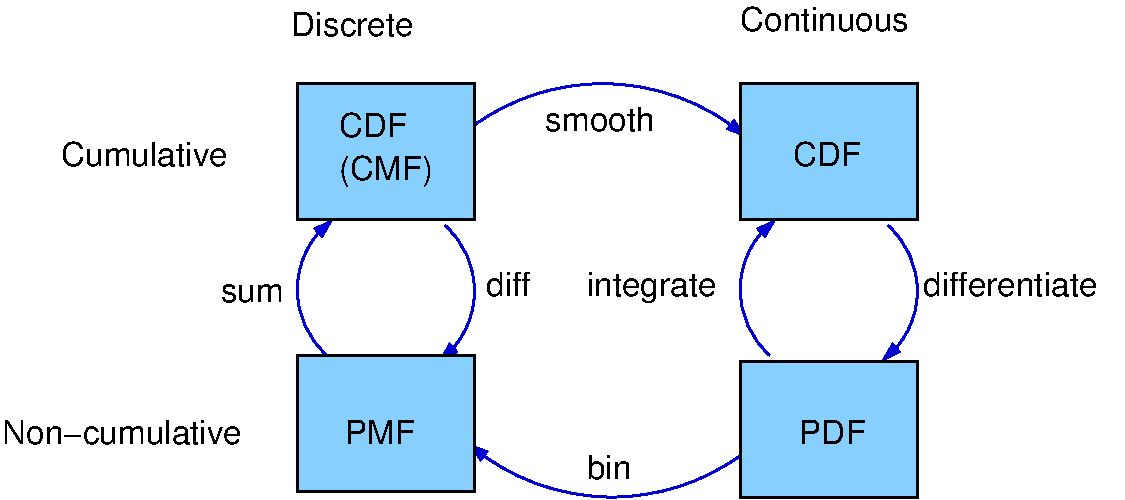
\includegraphics[height=2.2in]{figs/distribution_functions.pdf}}
\caption{A framework that relates representations of distribution
functions.}
\label{dist_framework}
\end{figure}

At this point we have seen PMFs, CDFs and PDFs; let's take a minute
to review.  Figure~\ref{dist_framework} shows how these functions relate
to each other.
\index{PMF}

We started with PMFs, which represent the probabilities for a discrete
set of values.  To get from a PMF to a CDF, we computed a cumulative sum.
To be more consistent, a discrete CDF should be called a cumulative mass
function (CMF), but as far as I can tell no one uses that term.
\index{CDF}

To get from a CDF to a PMF, you can compute differences in cumulative
probabilities.
\index{PDF}

Similarly, a PDF is the derivative of a continuous CDF; or, equivalently,
a CDF is the integral of a PDF.  But remember that a PDF maps from
values to probability densities; to get a probability, you have to
integrate.
\index{discrete}
\index{continuous}

To get from a discrete to a continuous distribution, you can perform
various kinds of smoothing.  One form of smoothing is to assume that
the data come from an analytic continuous distribution
(like exponential or normal) and to estimate the parameters of that
distribution.  And that's what Chapter~\ref{estimation} is about.
\index{exponential distribution}
\index{distribution!exponential}
\index{normal distribution}
\index{distribution!normal}
\index{Gaussian distribution}
\index{distribution!Gaussian}
\index{bin}

If you divide a PDF into a set of bins, you can generate a PMF that is
at least an approximation of the PDF.  We use this
technique in Chapter~\ref{estimation} to do Bayesian estimation.
\index{Bayesian estimation}
\index{estimation!Bayesian}

\begin{exercise}
Write a function called {\tt MakePmfFromCdf} that takes a Cdf object
and returns the corresponding Pmf object.

You can find a solution to this exercise in {\tt thinkstats.com/Pmf.py}.
\index{{\tt pmf.py}@{\tt Pmf.py}}

\end{exercise}

\section{Glossary}

\begin{description}

\item[skewness:] A characteristic of a distribution; intuitively, it
is a measure of how asymmetric the distribution is.
\index{skewness}

\item[robust:] A statistic is robust if it is relatively immune to the
  effect of outliers.
\index{robust}

\item[illusory superiority:] The tendency of people to imagine that
they are better than average.
\index{illusory superiority}
\index{fallacy!illusory superiority}

\item[random variable:] An object that represents a random process.
\index{random variable}
\index{variable!random}

\item[random variate:] A value generated by a random process.
\index{random variate}
\index{variate!random}

\item[PDF:] Probability density function, the derivative of a continuous CDF.
\index{PDF}
\index{probability density function}

\item[convolution:] An operation that computes the distribution of the
sum of values from two distributions. 
\index{convolution}

%\item[Chi-squared distribution:] The distribution of the sum of squared
%values from a normal distribution.

%\item[Degrees of freedom:] The number of values in a sample that are
%free to vary.

\item[Central Limit Theorem:] ``The supreme law of Unreason,'' according
to Sir Francis Galton, an early statistician.
\index{Central Limit Theorem}
\index{Galton, Francis}
\index{unreason, supreme law}

\end{description}


\chapter{Hypothesis testing}
\label{testing}
\index{hypothesis testing}
\index{apparent effect}

Exploring the data from the NSFG, we saw several ``apparent effects,''
including a number of differences between first babies and others.
So far we have taken these effects at face value; in this chapter,
finally, we put them to the test.
\index{National Survey of Family Growth}
\index{NSFG}

The fundamental question we want to address is whether these effects
are real.  For example, if we see a difference in the mean pregnancy
length for first babies and others, we want to know whether that
difference is real, or whether it occurred by chance.
\index{pregnancy length}
\index{length!pregnancy}

That question turns out to be hard to address directly, so we will
proceed in two steps.  First we will test whether the effect is {\bf
  significant}, then we will try to interpret the result
  as an answer to the original question.
\index{significant}

In the context of statistics, ``significant'' has a technical
definition that is different from its use in common language.
As defined earlier, an apparent effect is statistically
significant if it is unlikely to have occurred by chance.
\index{chance}

To make this more precise, we have to answer three questions:

\begin{enumerate}

\item What do we mean by ``chance''?

\item What do we mean by ``unlikely''?

\item What do we mean by ``effect''?

\end{enumerate}

All three of these questions are harder than they look.  Nevertheless,
there is a general structure that people use to test statistical
significance:

\begin{description}

\item[Null hypothesis:] The {\bf null hypothesis} is a model of the
  system based on the assumption that the apparent effect was actually
  due to chance.
\index{null hypothesis}

\item[p-value:] The {\bf p-value} is the probability of the apparent
  effect under the null hypothesis.
\index{p-value}

\item[Interpretation:] Based on the p-value, we conclude that the
  effect is either statistically significant, or not.

\end{description}

This process is called {\bf hypothesis testing}.  The underlying
logic is similar to a proof by contradiction.  To prove a mathematical
statement, A, you assume temporarily that A is false.  If that
assumption leads to a contradiction, you conclude that A must actually
be true.
\index{contradiction, proof by}

Similarly, to test a hypothesis like, ``This effect is real,'' we
assume, temporarily, that is is not.  That's the null hypothesis.
Based on that assumption, we compute the probability of the apparent
effect.  That's the p-value.  If the p-value is low enough, we
conclude that the null hypothesis is unlikely to be true.


\section{Testing a difference in means}
\index{mean, difference in}

One of the easiest hypotheses to test is an apparent difference in mean
between two groups.  In the NSFG data, we saw that the mean pregnancy
length for first babies is slightly longer, and the mean weight at
birth is slightly smaller.  Now we will see if those effects are
significant.
\index{National Survey of Family Growth}
\index{NSFG}
\index{pregnancy length}
\index{length!pregnancy}

For these examples, the null hypothesis is that the distributions
for the two groups are the same, and that the apparent difference is
due to chance.
\index{null hypothesis}

To compute p-values, we find the pooled distribution for all live
births (first babies and others), generate random samples that are
the same size as the observed samples, and compute the difference
in means under the null hypothesis.
\index{p-value}

If we generate a large number of samples, we can count how often the
difference in means (due to chance) is as big or bigger than the
difference we actually observed.  This fraction is the p-value.

For pregnancy length, we observed \n~=~4413 first babies and \m~=~4735
others, and the difference in mean was \mydelta~=~0.078 weeks.  To
approximate the p-value of this effect, I pooled the distributions,
generated samples with sizes \n~and \m~and computed the difference
in mean.
\index{resampling}

This is another example of resampling, because we are drawing a
random sample from a dataset that is, itself, a sample of the general
population.  I computed differences for 1000 sample pairs;
Figure~\ref{length_deltas_cdf} shows their distribution.

\begin{figure}
% hypothesis.py
\centerline{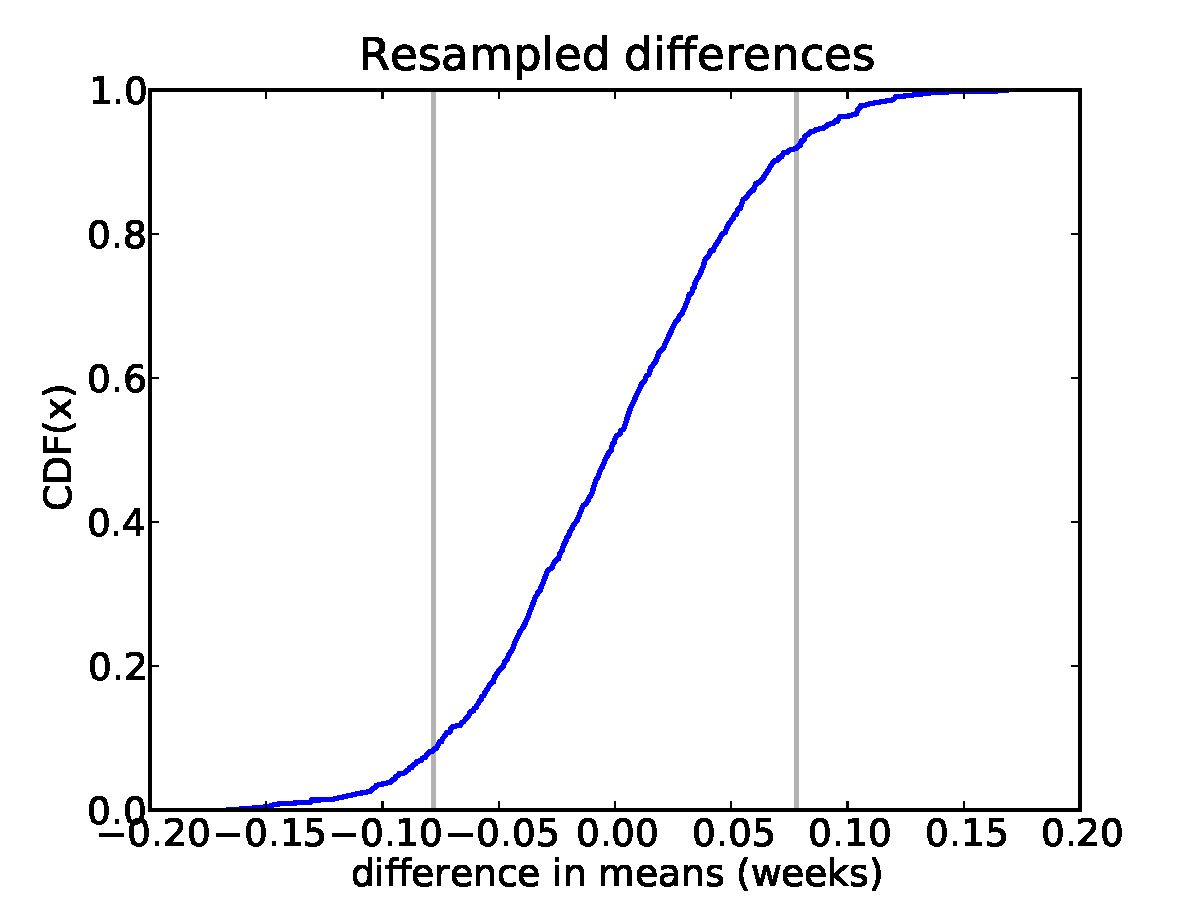
\includegraphics[height=2.5in]{figs/length_deltas_cdf.pdf}}
\caption{CDF of difference in mean for resampled data.}
\label{length_deltas_cdf}
\end{figure}

The mean difference is near 0, as you would expect with samples
from the same distribution.  The vertical lines show the cutoffs where
\x~=~\minus\mydelta~or \x~=~\mydelta.

Of 1000 sample pairs, there were 166 where the difference in mean
(positive or negative) was as big or bigger than \mydelta, so the
p-value is approximately 0.166.  In other words, we expect to see an
effect as big as \mydelta~about 17\% of the time, even if the actual
distribution for the two groups is the same.

So the apparent effect is not very likely, but is it unlikely enough?
I'll address that in the next section.

\begin{exercise}
In the NSFG dataset, the difference in mean weight for first
births is 2.0 ounces.  Compute the p-value of this difference.
\index{National Survey of Family Growth}
\index{NSFG}

Hint: for this kind of resampling it is important to sample
with replacement, so you should use {\tt random.choice} rather
than {\tt random.sample} (see Section~\ref{random}).
\index{resampling}
\index{random module}

You can start with the code I used to generate the results in this
section, which you can download from \url{http://thinkstats.com/hypothesis.py}.
\index{{\tt hypothesis.py}}

\end{exercise}


\section{Choosing a threshold}
\label{threshold}
\index{threshold}

In hypothesis testing we have to worry about two kinds of errors.
\index{false positive}
\index{false negative}
\index{error, Type I}
\index{error, Type II}

\begin{itemize}

\item A Type I error, also called a {\bf false positive}, is when we
  accept a hypothesis that is actually false; that is, we consider an
  effect significant when it was actually due to chance.

\item A Type II error, also called a {\bf false negative}, is when we
  reject a hypothesis that is actually true; that is, we attribute an
  effect to chance when it was actually real.

\end{itemize}

The most common approach to hypothesis testing is to choose a
threshold\footnote{Also known as a ``Significance criterion.''},
\myalpha, for the p-value and to accept as significant any effect with
a p-value less than \myalpha.  A common choice for \myalpha~is 5\%.
By this criterion, the apparent difference in pregnancy length for
first babies is not significant, but the difference in weight is.
\index{significance criterion}
\index{pregnancy length}
\index{length!pregnancy}

For this kind of hypothesis testing, we can compute the probability of
a false positive explicitly: it turns out to be \myalpha.

To see why, think about the definition of false positive---the chance
of accepting a hypothesis that is false---and the definition of a
p-value---the chance of generating the measured effect if the
hypothesis is false.

Putting these together, we can ask: if the hypothesis is false,
what is the chance of generating a measured effect that will be
considered significant with threshold \myalpha?  The answer is
\myalpha.

We can decrease the chance of a false positive by decreasing the
threshold.  For example, if the threshold is 1\%, there is only a 1\%
chance of a false positive.

But there is a price to pay: decreasing the threshold raises the
standard of evidence, which increases the chance of rejecting
a valid hypothesis.

In general there is a tradeoff between Type I and Type II errors.
The only way to decrease both at the same time is to increase the
sample size (or, in some cases, decrease measurement error).
\index{sample size}

\begin{exercise}
To investigate the effect of sample size on p-value, see what happens
if you discard half of the data from the NSFG.  Hint: use {\tt
  random.sample}.  What if you discard three-quarters of the data, and
so on?
\index{National Survey of Family Growth}
\index{NSFG}

What is the smallest sample size where the difference in mean birth
weight is still significant with \myalpha~=~5\%?  How much
larger does the sample size have to be with \myalpha~=~1\%?

You can start with the code I used to generate the results in this
section, which you can download from \url{http://thinkstats.com/hypothesis.py}.
\index{{\tt hypothesis.py}}

\end{exercise}


\section{Defining the effect}

When something unusual happens, people often say something like,
``Wow!  What were the chances of {\em that}?''  This question makes
sense because we have an intuitive sense that some things are more
likely than others.  But this intuition doesn't always hold up to
scrutiny.
\index{chance}
\index{coin}

For example, suppose I toss a coin 10 times, and after each toss I
write down H for heads and T for tails.  If the result was a sequence
like THHTHTTTHH, you wouldn't be too surprised.  But if the result was
HHHHHHHHHH, you would say something like, ``Wow!  What were the
chances of {\em that}?''

But in this example, the probability of the two sequences is the
same: one in 1024.  And the same is true for any other sequence.
So when we ask, ``What were the chances of {\em that},'' we have
to be careful about what we mean by ``that.''

For the NSFG data, I defined the effect as ``a difference in mean
(positive or negative) as big or bigger than \mydelta.''  By making
this choice, I decided to evaluate the magnitude of the difference,
ignoring the sign.
\index{National Survey of Family Growth}
\index{NSFG}

A test like that is called {\bf two-sided}, because we consider both
sides (positive and negative) in the distribution from
Figure~\ref{length_deltas_cdf}.  By using a two-sided test we are
testing the hypothesis that there is a significant difference between
the distributions, without specifying the sign of the difference.
\index{one-sided test}
\index{two-sided test}
\index{test!one-sided}
\index{test!two-sided}

The alternative is to use a {\bf one-sided} test, which asks whether
the mean for first babies is significantly {\em higher} than
the mean for others.  Because the hypothesis is more specific, the
p-value is lower---in this case it is roughly half.


\section{Interpreting the result}

At the beginning of this chapter I said that the question we want to
address is whether an apparent effect is real.  We started by defining
the null hypothesis, denoted \HH\sub{0}, which is the hypothesis that
the effect is not real.  Then we defined the p-value, which is
\Prob(\E|\HH\sub{0}), where \E~is an effect as big as or bigger
than the apparent effect.  Then we computed p-values and compared them
to a threshold, \myalpha.

That's a useful step, but it doesn't answer the original question,
which is whether the effect is real.  There are several ways to
interpret the result of a hypothesis test:

\begin{description}

\item[Classical:] In classical hypothesis testing, if a p-value
  is less than \myalpha, you can say that the effect is statistically
  significant, but you can't conclude that it's real.  This
  formulation is careful to avoid leaping to conclusions, but it is
  deeply unsatisfying.

\item[Practical:] In practice, people are not so formal.  In most
  science journals, researchers report p-values without apology, and
  readers interpret them as evidence that the apparent effect is real.
  The lower the p-value, the higher their confidence in this
  conclusion.
\index{Bayesian probability}

\item[Bayesian:] What we really want to know is \Prob(\HH\sub{A}|\E), 
  where \HH\sub{A} is the hypothesis that the effect is real.  
  By Bayes's theorem
  %
  \[ P(H_A \given E) = \frac{P(E \given H_A) \spa P(H_A)}{P(E)} \]
  %  
  where \Prob(\HH\sub{A}) is the prior probability of \HH\sub{A} before 
  we saw the
  effect, \Prob(\E|\HH\sub{A}) is the probability of seeing \E, 
  assuming that
  the effect is real, and \Prob(\E) is the probability of seeing 
  \E~under any hypothesis.  Since the effect is either real or it's not,
  
  \Eqn{ \Prob(\E) = \Prob(\E|\HH\sub{A}) \Prob(\HH\sub{A})~+~\Prob(\E|\HH\sub{0}) \Prob(\HH\sub{0}) }

\end{description}

As an example, I'll compute \Prob(\HH\sub{A}|E) for pregnancy
lengths in the NSFG.  We have already computed
\Prob(\E|\HH\sub{0})~=~0.166, so all we have to do is compute
\Prob(\E|\HH\sub{A}) and choose a value for the prior.
\index{prior probability}
\index{National Survey of Family Growth}
\index{NSFG}
\index{pregnancy length}
\index{length!pregnancy}

To compute \Prob(\E|\HH\sub{A}), we assume that the effect is
real---that is,
that the difference in mean duration, \mydelta, is actually what we
observed, 0.078.  (This way of formulating \HH\sub{A}~is a little bit
bogus.  I will explain and fix the problem in the next section.)

By generating 1000 sample pairs, one from each
distribution, I estimated \Prob(E|\HH\sub{A})~=~0.494.  With the prior
\Prob(\HH\sub{A})~=~0.5, the posterior probability of \HH\sub{A} is 0.748.
\index{posterior probability}
\index{update}

So if the prior probability of \HH\sub{A}~is 50\%, the updated
probability, taking into account the evidence from this dataset,
is almost 75\%.  It makes sense that the posterior
is higher, since the data provide some support for the hypothesis.
But it might seem surprising that the difference is so large,
especially since we found that the difference in means was not
statistically significant.

In fact, the method I used in this section is not quite right, and
it tends to overstate the impact of the evidence.  In the next section
we will correct this tendency.

\begin{exercise}
Using the data from the NSFG, what is the posterior probability that
the distribution of birth weights is different for first babies and
others?
\index{birth weight}
\index{weight!birth}
\index{National Survey of Family Growth}
\index{NSFG}

You can start with the code I used to generate the results in this
section, which you can download from \url{http://thinkstats.com/hypothesis.py}.
\index{{\tt hypothesis.py}}

\end{exercise}


\section{Cross-validation}
\index{cross-validation}

In the previous example, we used the dataset to formulate the
hypothesis \HH\sub{A}, and then we used the same dataset to test it.
That's not a good idea; it is too easy to generate misleading results.

The problem is that even when the null hypothesis is true, there is
likely to be some difference, \mydelta, between any two groups, just by
chance.  If we use the observed value of \mydelta~to formulate the
hypothesis, \Prob(\HH\sub{A}|\E) is likely to be high even when
\HH\sub{A}~is false.

We can address this problem with {\bf cross-validation}, which uses
one dataset to compute \mydelta~and a {\em different} dataset to
evaluate \HH\sub{A}.  The first dataset is called the {\bf training set};
the second is called the {\bf testing set}.
\index{training set}
\index{test set}
\index{cohort}
\index{cycle}

In a study like the NSFG, which studies a different cohort in each
cycle, we can use one cycle for training and another for testing.
Or we can partition the data into subsets (at random), then use
one for training and one for testing.
\index{National Survey of Family Growth}
\index{NSFG}

I implemented the second approach, dividing the Cycle 6 data roughly
in half.  I ran the test several times with different random partitions.
The average posterior probability was \Prob(\HH\sub{A}|\E)~=~0.621.
As expected, the impact of the evidence is smaller, partly because of
the smaller sample size in the test set, and also because we are no
longer using the same data for training and testing.

% t = [0.656, 0.622, 0.511, 0.651, 0.665]
% sum(t)/len(t)


\section{Reporting Bayesian probabilities}
\index{Bayesian probability}

In the previous section we chose the prior probability \Prob(\HH\sub{A})~=~0.5.
If we have a set of hypotheses and no reason to think one is more
likely than another, it is common to assign each the same probability.

Some people object to Bayesian probabilities because they depend on
prior probabilities, and people might not agree on
the right priors.  For people who expect scientific results to be
objective and universal, this property is deeply unsettling.
\index{subjective belief}
\index{belief}
\index{swamp}
\index{convergence}

One response to this objection is that, in practice, strong evidence
tends to swamp the effect of the prior, so people who start with
different priors will converge toward the same posterior
probability.
\index{likelihood ratio}
\index{Bayes factor}

Another option is to report just the {\bf likelihood ratio}, \Prob(E
| \HH\sub{A}) ~/~ \Prob(\E|\HH\sub{0}), rather than the
posterior probability.  That way readers can plug in whatever prior
they like and compute their own posteriors (no pun intended).  The
likelihood ratio is sometimes called a Bayes factor (see
\url{http://wikipedia.org/wiki/Bayes_factor}).

\begin{exercise}
If your prior probability for a hypothesis, \HH\sub{A}, is 0.3 and new
evidence becomes available that yields a likelihood ratio of 3
relative to the null hypothesis, \HH\sub{0}, what is your posterior
probability for \HH\sub{A}?
\index{null hypothesis}

% 0.3 * 3 / (0.3 * 3 + 0.7) = 0.6

\end{exercise}


\begin{exercise}
This exercise is adapted from MacKay, {\em Information
  Theory, Inference, and Learning Algorithms}:
\index{MacKay, David}

\begin{quote}

Two people have left traces of their own blood at the scene of a
crime.  A suspect, Oliver, is tested and found to have type O blood.
The blood groups of the two traces are found to be of type O (a common
type in the local population, having frequency 60\%) and of type AB (a
rare type, with frequency 1\%).  Do these data (the blood types found
at the scene) give evidence in favor of the proposition that
Oliver was one of the two people whose blood was found at the scene?

\end{quote}

Hint: Compute the likelihood ratio for this evidence; if it is greater
than 1, then the evidence is in favor of the proposition.
For a solution and discussion, see page 55 of MacKay's book.
\index{likelihood}

\end{exercise}


\section{Chi-square test}
\index{Chi-square test}

In Section~\ref{threshold} we concluded that the apparent difference
in mean pregnancy length for first babies and others was not
significant.  But in Section~\ref{relative.risk}, when we computed
relative risk, we saw that first babies are more likely to be early,
less likely to be on time, and more likely to be late.
\index{relative risk}
\index{pregnancy length}
\index{length!pregnancy}

So maybe the distributions have the same mean and different variance.
We could test the significance of the difference in variance, but
variances are less robust than means, and hypothesis tests for
variance often behave badly.
\index{mean}
\index{variance}
\index{hypothesis}

An alternative is to test a hypothesis that more directly reflects the
effect as it appears; that is, the hypothesis that first babies are
more likely to be early, less likely to be on time, and more likely to
be late.

We proceed in five easy steps:

\begin{enumerate}

\item We define a set of categories, called {\bf cells}, that each
  baby might fall into.  In this example, there are six cells because
  there are two groups (first babies and others) and three bins
  (early, on time or late).
\index{cell}

I'll use the definitions from Section~\ref{relative.risk}: a baby is
early if it is born during Week 37 or earlier, on time if it is born
during Week 38, 39 or 40, and late if it is born during Week 41 or
later.

\item We compute the number of babies we expect in each cell.  Under
  the null hypothesis, we assume that the distributions are the same
  for the two groups, so we can compute the pooled probabilities:
  \Prob(early), \Prob(ontime) and \Prob(late).

For first babies, we have \n~=~4413 samples, so under the null
hypothesis we expect \n~\Prob(early) first babies to be early,
\n~\Prob(ontime) to be on time, etc.  Likewise, we have \m~=~4735
other babies, so we expect \m~\Prob(early) other babies to be
early, etc.

\item For each cell we compute the deviation; that is, the difference
  between the observed value, \OO\sub{i}, and the expected value, \E\sub{i}.
\index{test statistic}
\index{chi-square statistic}

\item We compute some measure of the total deviation; this quantity
is called the {\bf test statistic}.  The most common
choice is the chi-square statistic:
%
\[ \chi^2 = \sum_i \frac{(O_i - E_i)^2}{E_i} \]
%
%% Consider using upper case chi, which is more strictly correct,
%% but harder to distinguish from X.

\item We can use a Monte Carlo simulation to compute the p-value,
  which is the probability of seeing a chi-square statistic as high
  as the observed value under the null hypothesis.
\index{simulation!Monte Carlo}
\index{Monte Carlo}

\end{enumerate}

When the chi-square statistic is used, this process is called a 
{\bf chi-square test}.  One feature of the chi-square test is that
the distribution of the test statistic can be computed analytically.
\index{chi-square test}
\index{analysis}

Using the data from the NSFG I computed \mychi\super{2}~=~91.64, which would
occur by chance about one time in 10,000.  I conclude that this result
is statistically significant, with one caution: again we used the
same dataset for exploration and testing.  It would be a good idea
to confirm this result with another dataset.
\index{National Survey of Family Growth}
\index{NSFG}

You can download the code I used in this section from
\url{http://thinkstats.com/chi.py}.
\index{{\tt chi.py}}

% See \url{http://en.wiktionary.org/wiki/voila}!


\begin{exercise}
Suppose you run a casino and you suspect that a customer has
replaced a die provided by the casino with a ``crooked die;'' that
is, one that has been tampered with to make one of the faces more
likely to come up than the others.  You apprehend the alleged
cheater and confiscate the die, but now you have to prove that it
is crooked.
\index{casino}
\index{dice}
\index{crooked die}

You roll the die 60 times and get the following results:

\begin{center}
\begin{tabular}{|l|c|c|c|c|c|c|}
\hline
Value     &  1  &  2  &  3  &  4  &  5  &  6  \\ 
\hline
\hline
Frequency &  8  &  9  &  19  &  6  &  8  &  10  \\
\hline
\end{tabular}
\end{center}

What is the chi-squared statistic for these values?  What is the
probability of seeing a chi-squared value as large by chance?

\end{exercise}




\section{Efficient resampling}
\index{resampling}

Anyone reading this book who has prior training in statistics probably
laughed when they saw Figure~\ref{length_deltas_cdf}, because I used a
lot of computer power to simulate something I could have figured out
analytically.
\index{analysis}
\index{pregnancy length}
\index{length!pregnancy}

Obviously mathematical analysis is not the focus of this book.  I am
willing to use computers to do things the ``dumb'' way, because I
think it is easier for beginners to understand simulations, and easier
to demonstrate that they are correct.  So as long as the simulations
don't take too long to run, I don't feel guilty for skipping the
analysis.

However, there are times when a little analysis can save a lot of
computing, and Figure~\ref{length_deltas_cdf} is one of those times.
\index{mean, difference in}

Remember that we were testing the observed difference in the mean between
pregnancy lengths for \n~=~4413 first babies and \m~=~4735 others.  We formed
the pooled distribution for all babies, drew samples with sizes \n~and
\m, and computed the difference in sample means.
\index{sample mean}

Instead, we could directly compute the distribution of the difference
in sample means.  To get started, let's think about what a sample mean
is: we draw \n~samples from a distribution, add them up, and
divide by \n.  If the distribution has mean \mymu~and variance
\sigmasq, then by the Central Limit Theorem, we know that the sum of
the samples is \mynormal (\n \mymu, \n \sigmasq).
\index{normal distribution}
\index{distribution!normal}
\index{Gaussian distribution}
\index{distribution!Gaussian}

To figure out the distribution of the sample means, we have to invoke
one of the properties of the normal distribution: if \X~is
\mynormal (\mymu, \sigmasq),

\Eqn{ \mya\X~+~\myb~\mysim~\mynormal(\mya \mymu~+~\myb, \mya\super{2} \sigmasq) }

When we divide by \n, \mya~=~1/\n and \myb~=~0, so

\X/\n~\mysim~\mynormal(\mymu /\n, \sigmasq/ \n\super{2})

So the distribution of the sample mean is \mynormal (\mymu, \sigmasq/\n).

To get the distribution of the difference between two sample means,
we invoke another property of the normal distribution: if \X\sub{1} is
\mynormal (\mymu\sub{1}, \mysigma\sub{1}\super{2}) and \X\sub{2} is
\mynormal (\mymu\sub{2}, \mysigma\sub{2}\super{2}),
%
\[ aX_1 + bX_2 \sim \normal (a\mu_1 + b\mu_2, 
                                 a^2\sigma_1^2 + b^2\sigma_2^2) \]
%
So as a special case:
%
\[ X_1 - X_2 \sim \normal (\mu_1 - \mu_2, 
                               \sigma_1^2 + \sigma_2^2) \]
%
Putting it all together, we conclude that the sample in
Figure~\ref{length_deltas_cdf} is drawn from 
\mynormal (0, \f \sigmasq), where \f~=~1/\n~+~1/\m.  Plugging in
\n~=~4413 and \m~=~4735, we expect the difference of sample means to be
\mynormal (0, 0.0032).
\index{p-value}

We can use {\tt erf.NormalCdf} to compute the p-value of the observed 
difference in the means:
%
\begin{verbatim}
delta = 0.078
sigma = math.sqrt(0.0032)
left = erf.NormalCdf(-delta, 0.0, sigma)
right = 1 - erf.NormalCdf(delta, 0.0, sigma)
\end{verbatim}

The sum of the left and right tails is the p-value, 0.168, which is
pretty close to what we estimated by resampling, 0.166. 
You can download the code I used in this section from
\url{http://thinkstats.com/hypothesis_analytic.py}
\index{{\tt hypothesis\_analytic.py}}


\section{Power}
\index{power}

When the result of a hypothesis test is negative (that is, the effect is
not statistically significant), can we conclude that the effect is not
real?  That depends on the power of the test.

Statistical {\bf power} is the probability that the test will be
positive if the null hypothesis is false.  In general, the power of a
test depends on the sample size, the magnitude of the effect, and the
threshold \myalpha.

\begin{exercise}
What is the power of the test in Section~\ref{threshold}, using
\myalpha~=~0.05 and assuming that the actual difference between the
means is 0.078 weeks?

You can estimate power by generating random samples from distributions
with the given difference in the mean, testing the observed difference
in the mean, and counting the number of positive tests.

What is the power of the test with \myalpha~=~0.10?

\end{exercise}

One way to report the power of a test, along with a negative result,
is to say something like, ``If the apparent effect were as large
as \x, this test would reject the null hypothesis with probability \p.''


%\section{Discussion}

%Pitfalls:

%1) Exploring and then testing

%2) Multiple tests

%3) Publication bias


%Solutions:

%1) two phases: exploratory and testing, on different data (possibly a subset)

%2) Holm-Bonferroni method

%3) publish everything and wait for consensus




\section{Glossary}

\begin{description}

\item[significant:] An effect is statistically significant if it is unlikely
to occur by chance.
\index{significant}

\item[null hypothesis:] A model of a system based on the assumption that
an apparent effect is due to chance.
\index{null hypothesis}

\item[p-value:] The probability that an effect could occur by chance.
\index{p-value}

\item[hypothesis testing:] The process of determining whether an apparent
effect is statistically significant.
\index{hypothesis testing}

\item[false positive:] The conclusion that an effect is real when it is not.
\index{false positive}

\item[false negative:] The conclusion that an effect is due to chance when it
is not.
\index{false negative}

\item[two-sided test:] A test that asks, ``What is the chance of an effect
as big as the observed effect, positive or negative?''

\item[one-sided test:] A test that asks, ``What is the chance of an effect
as big as the observed effect, and with the same sign?''
\index{one-sided test}
\index{two-sided test}
\index{test!one-sided}
\index{test!two-sided}

\item[cross-validation:] A process of hypothesis testing that uses one
dataset for exploratory data analysis and another dataset for testing.
\index{cross-validation}

\item[training set:] A dataset used to formulate a hypothesis for testing.
\index{training set}

\item[testing set:] A dataset used for testing.
\index{testing set}

\item[test statistic:] A statistic used to measure the deviation of an
apparent effect from what is expected by chance.
\index{test statistic}

\item[chi-square test:] A test that uses the chi-square statistic as
the test statistic.
\index{ch-square test}

\item[likelihood ratio:] The ratio of \Prob(\E|\A) to \Prob(\E|\B) 
  for two hypotheses \A~and \B, which is a way to report
  results from a Bayesian analysis without depending on priors.
  \index{likelihood ratio}

\item[cell:] In a chi-square test, the categories the observations are
divided into.
\index{cell}

\item[power:] The probability that a test will reject the null hypothesis
if it is false.
\index{power}

\end{description}



\chapter{Estimation}
\label{estimation}
\index{estimation}

\section{The estimation game}

Let's play a game.  I'll think of a distribution, and you have to guess
what it is.  We'll start out easy and work our way up.
\index{normal distribution}
\index{distribution!normal}
\index{Gaussian distribution}
\index{distribution!Gaussian}

{\em I'm thinking of a distribution.}  I'll give you two hints; it's a
normal distribution, and here's a random sample drawn from it:

\{\minus0.441, 1.774, \minus0.101, \minus1.138, 2.975, \minus2.138\}

What do you think is the mean parameter, \mymu, of this distribution?
\index{mean}
\index{parameter}

One choice is to use the sample mean to estimate \mymu.  Up
until now we have used the symbol \mymu~for both the sample mean and
the mean parameter, but now to distinguish them I will use \myxbar~for 
the sample mean.  In this example, \myxbar~is 0.155, so it would
be reasonable to guess \mymu~=~0.155.

This process is called {\bf estimation}, and the statistic we used
(the sample mean) is called an {\bf estimator}.
\index{estimator}

Using the sample mean to estimate \mymu~is so obvious that it is hard
to imagine a reasonable alternative.  But suppose we change the game by
introducing outliers.  
\index{normal distribution}
\index{distribution!normal}
\index{Gaussian distribution}
\index{distribution!Gaussian}

{\em I'm thinking of a distribution.}  It's a normal distribution, and
here's a sample that was collected by an unreliable surveyor who
occasionally puts the decimal point in the wrong place.

\{\minus0.441, 1.774, \minus0.101, \minus1.138, 2.975, \minus213.8\}

Now what's your estimate of \mymu?  If you use the sample mean your
guess is \minus35.12.  Is that the best choice?  What are the alternatives?
\index{outlier}

One option is to identify and discard outliers, then compute the sample
mean of the rest.  Another option is to use the median as an estimator.
\index{median}

Which estimator is the best depends on the circumstances (for example,
whether there are outliers) and on what the goal is.  Are you
trying to minimize errors, or maximize your chance of getting the
right answer?
\index{error}
\index{MSE}
\index{mean squared error}

If there are no outliers, the sample mean minimizes the {\bf mean squared
error} (MSE).  If we play the game many times, and each time
compute the error \myxbar~\minus~\mymu, the sample mean minimizes
%
\[ MSE = \frac{1}{m} \sum (\xbar - \mu)^2 \]
%
Where \m~is the number of times you play the estimation game (not to
be confused with \n, which is the size of the sample used to compute
\myxbar). 

Minimizing MSE is a nice property, but it's not always the best
strategy.  For example, suppose we are estimating the distribution of
wind speeds at a building site.  If we guess too high, we might
overbuild the structure, increasing its cost.  But if we guess too
low, the building might collapse.  Because cost as a function of
error is asymmetric, minimizing MSE is not the best strategy.
\index{prediction}

As another example, suppose I roll three six-sided dice and ask you
to predict the total.  If you get it exactly right, you get a prize;
otherwise you get nothing.  In this case the value that minimizes MSE
is 10.5, but that would be a terrible guess.  For this game, you
want an estimator that has the highest chance of being right, which is
a {\bf maximum likelihood estimator} (MLE).  If you pick 10 or 11, your
chance of winning is 1 in 8, and that's the best you can do.
\index{MLE}
\index{maximum likelihood estimator}

\begin{exercise}
Write a function that draws 6 values from a normal distribution with
\mymu~=~0 and \mysigma~=~1.  Use the sample mean to estimate \mymu~and
compute the error \myxbar~\minus~\mymu.  Run the function 1000 times and
compute MSE.
\index{normal distribution}
\index{distribution!normal}
\index{Gaussian distribution}
\index{distribution!Gaussian}

Now modify the program to use the median as an
estimator.  Compute MSE again and compare to the MSE for \myxbar.
\index{mean}
\index{median}
\index{MSE}

\end{exercise}


\section{Guess the variance}
\index{variance}
\index{normal distribution}
\index{distribution!normal}
\index{Gaussian distribution}
\index{distribution!Gaussian}

{\em I'm thinking of a distribution.}  It's a normal distribution, and 
here's a (familiar) sample:

\{\minus0.441, 1.774, \minus0.101, \minus1.138, 2.975, \minus2.138\}

What do you think is the variance, \sigmasq, of my distribution?
Again, the obvious choice is to use the sample variance as an estimator.
I will use \Ssq to denote the sample variance, to distinguish from the
unknown parameter \sigmasq.
%
\[ S^2 = \frac{1}{n} \sum (x_i - \xbar)^2 \] 
%
For large samples, \Ssq is an adequate estimator, but for small
samples it tends to be too low.  Because of this unfortunate
property, it is called a {\bf biased} estimator.
\index{sample variance}
\index{biased estimator}
\index{estimator!biased}
\index{unbiased estimator}
\index{estimator!unbiased}


An estimator is {\bf unbiased} if the expected total (or mean) error,
after many iterations of the estimation game, is 0.
Fortunately, there is another simple statistic that is an unbiased
estimator of \sigmasq:
%
\[ S_{n-1}^2 = \frac{1}{n-1} \sum (x_i - \xbar)^2 \] 
%
The biggest problem with this estimator is that its name and symbol
are used inconsistently.  The name ``sample variance'' can refer to
either \Ssq or \Snsq, and the symbol \Ssq is used
for either or both.

For an explanation of why \Ssq is biased, and a proof that
\Snsq is unbiased, see
\url{http://wikipedia.org/wiki/Bias_of_an_estimator}.

\begin{exercise}
Write a function that draws 6 values from a normal distribution with
\mymu~~=~~0 and \mysigma~~=~~1.  Use the sample variance to estimate
\sigmasq~and compute the error \Ssq~\minus~\mysigma\super{2}.
Run the function 1000 times and compute mean error (not squared).
\index{normal distribution}
\index{distribution!normal}
\index{Gaussian distribution}
\index{distribution!Gaussian}

Now modify the program to use the unbiased estimator \Snsq.
Compute the mean error again and see if it converges to zero as you
increase the number of games.

\end{exercise}


\section{Understanding errors}
\index{error}

Before we go on, let's clear up a common source of confusion.
Properties like MSE and bias are long-term expectations based on
many iterations of the estimation game.

While you are playing the game, you don't know the errors.  That is,
if I give you a sample and ask you to estimate a parameter, you
can compute the value of the estimator, but you can't compute the
error.  If you could, you wouldn't need the estimator!

The reason we talk about estimation error is to describe the behavior
of different estimators in the long run.  In this chapter we run
experiments to examine those behaviors; these experiments are
artificial in the sense that we know the actual values of the
parameters, so we can compute errors.  But when you work with
real data, you don't, so you can't.

Now let's get back to the game.


\section{Exponential distributions}
\index{exponential distribution}
\index{distribution!exponential}

{\em I'm thinking of a distribution.}  It's an exponential distribution, and 
here's a sample:

\{5.384, 4.493, 19.198, 2.790, 6.122, 12.844\}

What do you think is the parameter, \mylambda, of this distribution?
\index{parameter}
\index{mean}

\newcommand{\lamhat}{\hat{\lambda}}
\newcommand{\lamhatmed}{\hat{\lambda}_{1/2}}

In general, the mean of an exponential distribution is 1/\mylambda,
so working backwards, we might choose

\Eqn{ $\lamhat$ = 1 / \myxbar }

It is common to use hat notation for estimators, so $\lamhat$ is an
estimator of \mylambda.  And not just any estimator; it is also the
MLE estimator\footnote{See
\url{http://wikipedia.org/wiki/Exponential_distribution\#Maximum_likelihood}.}.
So if you want to maximize your chance of guessing \mylambda~exactly,
$\lamhat$ is the way to go.
\index{MLE}
\index{maximum likelihood estimator}

But we know that \myxbar~is not robust in the presence of outliers, so
we expect $\lamhat$ to have the same problem.
\index{robust}
\index{outlier}

Maybe we can find an alternative based on the sample median.  Remember
that the median of an exponential distribution is log(2) / \mylambda,
so working backwards again, we can define an estimator
%
\[ \lamhatmed = \log(2) / \mu_{1/2} \]
%
where \mymu \sub{1/2} is the sample median.
\index{median}

\begin{exercise}
Run an experiment to see which of $\lamhat$ and $\lamhatmed$ yields
lower MSE.  Test whether either of them is biased.
\index{biased estimator}

%Note: in this kind of experiment, you start with a known value for
%the parameter and generate a simulated data set, so you can compute
%errors.  But remember that in non-experimental conditions you can't
%compute MSE or check for bias.

\end{exercise}


\section{Confidence intervals}
\index{confidence interval}
\index{interval!confidence}
\index{point estimate}

So far we have looked at estimators that generate single values, known
as {\bf point estimates}.  For many problems, we might prefer an interval
that specifies an upper and lower bound on the unknown parameter.

Or, more generally, we might want that whole distribution; that is,
the range of values the parameter could have, and for each value in
the range, a notion of how likely it is.

Let's start with {\bf confidence intervals}.
\index{exponential distribution}
\index{distribution!exponential}

{\em I'm thinking of a distribution.}  It's an exponential distribution, and 
here's a sample:

\{5.384, 4.493, 19.198, 2.790, 6.122, 12.844\}

I want you to give me a range of values that you think is likely to
contain the unknown parameter \mylambda.  More specifically, I want
a 90\% confidence interval, which means that if we play this game over
and over, your interval will contain \mylambda~90\% of the time.

It turns out that this version of the game is hard, so I'm going
to tell you the answer, and all you have to do is test it.

Confidence intervals are usually described in terms of the miss rate,
\myalpha, so a 90\% confidence interval has miss rate \myalpha~=~0.1.
The confidence interval for the \mylambda~parameter of an exponential
distribution is
%
\[ \left( \lamhat \frac{\chi^2(2n, 1-\alpha/2)}{2n},
      \lamhat \frac{\chi^2(2n, \alpha/2)}{2n} \right) \]
%
where \n~is the sample size, $\lamhat$ is the mean-based estimator
from the previous section, and \mychi\super{2}(\kk, \x) is the CDF of a
chi-squared distribution with \kk~degrees of freedom, evaluated at \x
(see \url{http://wikipedia.org/wiki/Chi-square_distribution}).
\index{chi-square distribution}
\index{distribution!chi-square}

In general, confidence intervals are hard to compute analytically, but
relatively easy to estimate using simulation.  But first we need
to talk about Bayesian estimation.
\index{Bayesian estimation}
\index{estimation!Bayesian}


%\begin{exercise}
%\label{expo_ci}

%Write a function that computes a 90\% confidence interval for
%\mylambda, given $\lamhat$, \n~and \myalpha.

%Run an experiment that checks whether the confidence interval has the
%property we expect; that is, the interval should contain the actual
%value 90\% of the time.

%To do that, write a function that takes a value for \mylambda,
%generates a sample of six values, computes a 90\% confidence interval,
%and checks whether the interval contains the \mylambda.  Run the
%function 1000 times and count the number of hits.

%\end{exercise}


\section{Bayesian estimation}

If you collect a sample and compute a 90\% confidence interval, it is
tempting to say that the true value of the parameter has a 90\% chance
of falling in the interval.  But from a frequentist point of view,
that is not correct because the parameter is an unknown but fixed
value.  It is either in the interval you computed or not, so the
frequentist definition of probability doesn't apply.
\index{parameter}
\index{frequentism}
\index{Bayesianism}

So let's try a different version of the game.
\index{exponential distribution}
\index{distribution!exponential}
\index{uniform distribution}
\index{distribution!uniform}

{\em I'm thinking of a distribution.}  It's an exponential
distribution, and I chose \mylambda~from a uniform distribution
between 0.5 and 1.5.  Here's a sample, which I'll call \X:

\{2.675, 0.198, 1.152, 0.787, 2.717, 4.269\}

Based on this sample, what value of \mylambda~do you think I chose?

In this version of the game, \mylambda~{\em is} a random quantity, so we
can reasonably talk about its distribution, and we can compute it
easily using Bayes's theorem.

Here are the steps:

\begin{enumerate}

\item Divide the range (0.5, 1.5) into a set of equal-sized bins.
For each bin, we define \HH\sub{i}, which is the hypothesis that the
actual value of \mylambda~falls in the \ii~th bin.
Since \mylambda~was drawn from a uniform distribution, the prior
probability, \Prob(\HH\sub{i}), is the same for all \ii.

\item For each hypothesis, we compute the likelihood, \Prob(\X|\HH\sub{i}),
which is the chance of drawing the sample \X given \HH\sub{i}.
%
\[ P(X \given H_i) = \prod_j \mathrm{expo}(\lambda_i, x_j)  \]
%
where expo(\mylambda, \x) is a function that
computes the PDF of the exponential distribution with parameter \mylambda,
evaluated at \x.  
%
\[ PDF_{expo}(\lambda, x) = \lambda e^{-\lambda x}\]
%
The symbol $\prod$ represents the product of a sequence (see
\url{http://wikipedia.org/wiki/Multiplication#Capital_Pi_notation}).

\item Then by Bayes's theorem the posterior distribution is

\Eqn{ \Prob(\HH\sub{i}|\X) =  \Prob(\HH\sub{i}) \Prob(\X|\HH\sub{i}) /\f }

where \f is the normalization factor
%
\[ f = \sum_i P(H_i) P(X \given H_i) \]
%
\end{enumerate}

Given a posterior distribution, it is easy to compute a confidence
interval.  For example, to compute a 90\% CI, you can
use the 5th and 95th percentiles of the posterior.
\index{credible interval}
\index{interval!credible}

Bayesian confidence intervals are sometimes called {\bf credible
intervals}; for a discussion of the differences, see
\url{http://wikipedia.org/wiki/Credible_interval}.


\section{Implementing Bayesian estimation}

To represent the prior distribution, we could use a Pmf, Cdf, or
any other representation of a distribution, but since we want to
map from a hypothesis to a probability, a Pmf is a natural choice.
\index{Pmf object}
\index{prior}
\index{posterior}

Each value in the Pmf represents a hypothesis; for example, the
value 0.5 represents the hypothesis that \mylambda~is 0.5.
In the prior distribution, all hypotheses have the same probability.
So we can construct the prior like this:
%
\begin{verbatim}
def MakeUniformSuite(low, high, steps):
    hypos = [low + (high-low) * i / (steps-1.0) for i in range(steps)]
    pmf = Pmf.MakePmfFromList(hypos)
    return pmf
\end{verbatim}

This function makes and returns a Pmf that represents a 
collection of related hypotheses, called a {\bf suite}.  Each hypothesis
has the same probability, so the distribution is {\bf uniform}.
\index{uniform distribution}
\index{distribution!uniform}
\index{suite}

The arguments {\tt low} and {\tt high} specify the range of values;
{\tt steps} is the number of hypotheses.
\index{update}

To perform the update, we take a suite of hypotheses and a body of
evidence:
%
\begin{verbatim}
def Update(suite, evidence):
    for hypo in suite.Values():
        likelihood = Likelihood(evidence, hypo)
        suite.Mult(hypo, likelihood)
    suite.Normalize()
\end{verbatim}

For each hypothesis in the suite, we multiply the prior probability
by the likelihood of the evidence.  Then we normalize the suite.

In this function, {\tt suite} has to be a Pmf, but {\tt evidence}
can be any type, as long as {\tt Likelihood} knows how to interpret it.
\index{likelihood}

Here's the likelihood function:
%
\begin{verbatim}
def Likelihood(evidence, hypo):
    param = hypo
    likelihood = 1
    for x in evidence:
        likelihood *= ExpoPdf(x, param)

    return likelihood
\end{verbatim}

In {\tt Likelihood} we assume that {\tt evidence} is a sample
from an exponential distribution and compute the product in the
previous section.
\index{exponential distribution}
\index{distribution!exponential}
\index{PDF}

{\tt ExpoPdf} evaluates the PDF of the exponential distribution
at {\tt x}:
%
\begin{verbatim}
def ExpoPdf(x, param):
    p = param * math.exp(-param * x)
    return p
\end{verbatim}

Putting it all together, here's the code that creates the prior
and computes the posterior:
%
\begin{verbatim}
evidence = [2.675, 0.198, 1.152, 0.787, 2.717, 4.269]
prior = MakeUniformSuite(0.5, 1.5, 100)
posterior = prior.Copy()
Update(posterior, evidence)
\end{verbatim}

You can download the code in this section from
\url{http://thinkstats.com/estimate.py}.
\index{{\tt estimate.py}}

When I think of Bayesian estimation, I imagine a room full of people,
where each person has a different guess about whatever you are trying
to estimate.  So in this example they each have a guess about the
correct value of \mylambda.

Initially, each person has a degree of confidence about their own hypothesis.
After seeing the evidence, each person updates their confidence based on
\Prob(\E|\HH), the likelihood of the evidence, given their hypothesis.

Most often the likelihood function computes a
probability, which is at most 1, so initially everyone's confidence
goes down (or stays the same).  But then we normalize, which increases
everyone's confidence.

So the net effect is that some people get more confident, and some less,
depending on the relative likelihood of their hypothesis.


\section{Censored data}
\label{censored}
\index{censored data}
\index{MacKay, David}

The following problem appears in Chapter 3 of David MacKay's
{\em Information Theory, Inference and Learning
  Algorithms}, which you can download from
\url{http://www.inference.phy.cam.ac.uk/mackay/itprnn/ps/}.

\begin{quote}
Unstable particles are emitted from a source and decay at a distance
\x, a real number that has an exponential probability distribution
with [parameter] \mylambda.  Decay events can
only be observed if they occur in a window extending from \x~=~1 cm to
\x~=~20 cm.  \n~decays are observed at locations \{ \x\sub{1}, ... , \x\sub{N}
\}.  What is \mylambda?
\index{exponential distribution}
\index{distribution!exponential}
\index{particles}
\index{unstable particles}
\index{decay}

\end{quote}

This is an example of an estimation problem with {\bf censored data};
that is, we know that some data are systematically excluded.

One of the strengths of Bayesian estimation is that it can deal with
censored data with relative ease.  We can use the method from the
previous section with only one change: we have to replace
PDF\sub{expo} with the conditional distribution:
%
\[ \PDF_{cond}(\lambda, x) = \lambda e^{-\lambda x} / Z(\lambda)  \]
%
for 1~<~\x~<~20, and 0 otherwise, with
%
\[ Z(\lambda) = \int_1^{20} \lambda e^{-\lambda x} \spa dx = 
e^{-\lambda} - e^{-20 \lambda}  \]
%
You might remember Z(\mylambda) from Exercise~\ref{expo_pdf}.  I told
you to keep it handy.

\begin{exercise}
Download \url{http://thinkstats.com/estimate.py}, which contains the code
from the previous section, and make a copy named {\tt decay.py}.
\index{{\tt estimate.py}}

Modify {\tt decay.py} to compute the posterior distribution of
\mylambda~for the sample \X~=~\{1.5, 2, 3, 4, 5, 12\}.  For
the prior you can use a uniform distribution between 0
and 1.5 (not including 0).
\index{uniform distribution}
\index{distribution!uniform}

You can download a solution to this problem from
\url{http://thinkstats.com/decay.py}.
\index{{\tt decay.py}}

\end{exercise}


\begin{exercise}
In the 2008 Minnesota Senate race the final vote count was 1,212,629
votes for Al Franken and 1,212,317 votes for Norm Coleman.  Franken
was declared the winner, but as Charles Seife points out in {\it
  Proofiness}, the margin of victory was much smaller than the margin
of error, so the result should have been considered a tie.
\index{Coleman, Norm}
\index{Franken, Al}
\index{Minnesota Senate Race}
\index{Seife, Charles}
\index{Proofiness@{\em Proofiness}}
\index{margin of victory}
\index{margin of error}

Assuming that there is a chance that any vote might be lost and a chance
that any vote might be double-counted, what is the probability that
Coleman actually received more votes?

Hint: you will have to fill in some details to model the error process.

\end{exercise}


\section{The locomotive problem}
\index{locomotive problem}
\index{Mosteller, Frederick}
\index{German tank problem}

The locomotive problem is a classic estimation problem also
known as the ``German tank problem.''  Here is the version
that appears in Mosteller, {\it Fifty Challenging Problems in
  Probability}:

\begin{quote}
``A railroad numbers its locomotives in order 1..N.  One day you see a
locomotive with the number 60.  Estimate how many locomotives the
railroad has.''
\end{quote}

Before you read the rest of this section, try to answer these
questions:

\begin{enumerate}

\item For a given estimate, \mynhat, what is the likelihood of the
  evidence, \Prob(\E|\mynhat)?  What is the maximum likelihood estimator?
\index{MLE}
\index{maximum likelihood estimator}

\item If we see train \ii~it seems reasonable that we would guess
  some multiple of \ii~so let's assume \mynhat~=~\mya \ii.  What value of
  \mya~minimizes mean squared error?
\index{MSE}
\index{mean squared error}

\item Still assuming that \mynhat~=~\mya \ii~can you find a value of \
\mya~that makes \mynhat~an unbiased estimator?
\index{unbiased estimator}
\index{estimator!unbiased}

\item For what value of N is 60 the average value?

\item What is the Bayesian posterior distribution assuming a prior
distribution that is uniform from 1 to 200?
\index{uniform distribution}
\index{distribution!uniform}
\index{posterior distribution}

\end{enumerate}

For best results, you should take some time to work on these questions
before you continue.

For a given estimate, \mynhat, the likelihood of seeing train \ii~is
1/$\nhat$ if \ii~\myle~$\nhat$, and 0 otherwise.  So the MLE is 
\mynhat~=~\ii.  
In other words, if you see train 60 and you want to maximize your
chance of getting the answer exactly right, you should guess that there
are 60 trains.

But this estimator doesn't do very well in terms of MSE.  We can do
better by choosing \mynhat~=~\mya\ii; all we have to do is find a good
value for \mya.

Suppose that there are, in fact, \N~trains.  Each time we play
the estimation game, we see train \ii~and guess \mya\ii, so the squared
error is (\mya\ii~\minus~\N)\super{2}.

If we play the game \N~times and see each train once, the mean
squared error is 
%
\[ MSE = \frac{1}{N} \sum_{i=1}^N (ai - N)^2 \]
%
To minimize MSE, we take the derivative with respect to \mya:
%
\[ \frac{d MSE}{da} = \frac{1}{N} \sum_{i=1}^N 2i (ai - N) = 0 \]
%
And solve for \mya.
%
\[ a = \frac{3N}{2N+1} \]
%
At first glance, that doesn't seem very useful, because \N~appears on
the right-hand side, which suggests that we need to know \N~to choose
\mya, but if we knew \N, we wouldn't need an estimator in the first place.

However, for large values of \N, the optimal value for \mya~converges
to 3/2, so we could choose \mynhat~=~3\ii / 2.

To find an unbiased estimator, we can compute the mean error (ME):
%
\[ ME = \frac{1}{N} \sum_{i=1}^N (ai - N) \]
%
And find the value of \mya~that yields ME~=~0, which turns out to be
%
\[ a = \frac{2N}{N-1}\]
%
For large values of \N, \mya~converges to 2, so we could choose
\mynhat~=~2\ii.

So far we have generated three estimators, \ii, 3\ii/2, and 2\ii,
that have the properties of maximizing likelihood, minimizing squared
error, and being unbiased.

Yet another way to generate an estimator is to choose the value
that makes the population mean equal the sample mean.  If we see train
\ii, the sample mean is just \ii; the train population that has the
same mean is \mynhat~=~2\ii~\minus~1.

\begin{figure}
% locomotive.py
\centerline{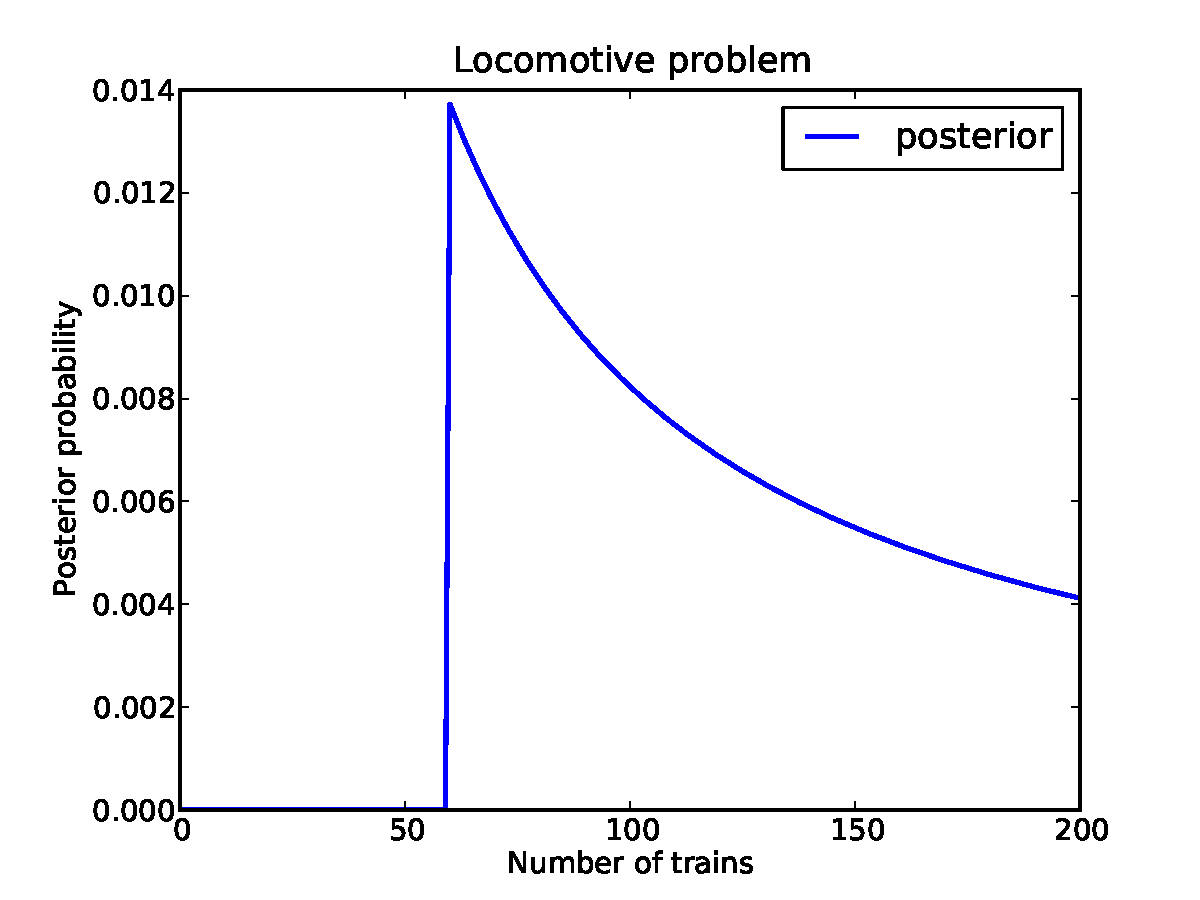
\includegraphics[height=2.5in]{figs/locomotive.pdf}}
\caption{Posterior distribution of the number of trains.}
\label{locomotive}
\end{figure}

Finally, to compute the Bayesian posterior distribution, we compute
%
\[ P(H_n \given i) = \frac{P(i \given H_n) P(H_n)}{P(i)} \]
%
Where \HH\sub{n} is the hypothesis that there are \n~trains, and \ii~is
the evidence: we saw train \ii.  Again, \Prob(\ii|\HH\sub{n})
is 1/\n~if \ii~< \n, and 0 otherwise.  The normalizing constant,
\Prob(\ii), is just the sum of the numerators for each hypothesis.
\index{Bayesian estimation}
\index{prior distribution}

If the prior distribution is uniform from 1 to 200, we start with 200
hypotheses and compute the likelihood for each.  You can download an
implementation from
\url{http://thinkstats.com/locomotive.py}.  Figure~\ref{locomotive} shows
what the result looks like.
\index{{\tt locomotive.py}}
\index{uniform distribution}
\index{distribution!uniform}

The 90\% credible interval for this posterior is [63, 189], which
is still quite wide.  Seeing one train doesn't provide strong evidence
for any of the hypotheses (although it does rule out the hypotheses
with \n~<~\ii).
\index{credible interval}

If we start with a different prior, the posterior is significantly
different, which helps to explain why the other estimators are so
diverse.

One way to think of different estimators is that they are implicitly
based on different priors.  If there is enough evidence to swamp the
priors, then all estimators tend to converge; otherwise, as in this
case, there is no single estimator that has all of the properties we
might want.

\begin{exercise}
Generalize \verb"locomotive.py" to handle the case where you
see more than one train.  You should only have to
change a few lines of code.
\index{{\tt locomotive.py}}

See if you can answer the other questions for the case where you
see more than one train.  You can find a discussion of the problem
and several solutions at
\url{http://wikipedia.org/wiki/German_tank_problem}.

\end{exercise}

\section{Glossary}

\begin{description}

\item[estimation:] The process of inferring the parameters of a distribution
from a sample.
\index{estimation}

\item[estimator:] A statistic used to estimate a parameter.
\index{estimation}

\item[mean squared error:] A measure of estimation error.
\index{mean squared error}
\index{MSE}

\item[maximum likelihood estimator:] An estimator that computes the
point estimate with the highest likelihood.
\index{MLE}
\index{maximum likelihood estimator}

\item[bias:] The tendency of an estimator to be above or below the actual
value of the parameter, when averaged over repeated samples.
\index{biased estimator}

\item[point estimate:] An estimate expressed as a single value.
\index{point estimation}

\item[confidence interval:] An estimate expressed as an interval with a
given probability of containing the true value of the parameter.
\index{confidence interval}
\index{interval!confidence}

\item[credible interval:] Another name for a Bayesian confidence interval.
\index{credible interval}
\index{interval!credible}

\item[censored data:] A dataset sampled in a way that systematically
excludes some data.
\index{censored data}

\end{description}


\chapter{Correlation}

\section{Standard scores}

In this chapter we look at relationships between variables.  For
example, we have a sense that height is related to weight; people who
are taller tend to be heavier.  {\bf Correlation} is a description of
this kind of relationship.
\index{correlation}

A challenge in measuring correlation is that the variables we want
to compare might not be expressed in the same units.  For example, height
might be in centimeters and weight in kilograms.  And even if they are
in the same units, they come from different distributions.
\index{units}

There are two common solutions to these problems:

\begin{enumerate}

\item Transform all values to {\bf standard scores}.  This leads to
the Pearson coefficient of correlation.
\index{standard scores}
\index{Pearson coefficient of correlation}
\index{Spearman coefficient of correlation}
\index{coefficient!correlation}

\item Transform all values to their percentile ranks.  This
leads to the Spearman coefficient.
\index{rank}
\index{percentile rank}

\end{enumerate}

If \X~is a series of values, \xsubi, we can convert to standard
scores by subtracting the mean and dividing by the standard deviation:
z\sub{i}~=~(x\sub{i}~\minus~\mymu) / \mysigma.
\index{mean}
\index{standard deviation}

The numerator is a deviation: the distance from the mean.  Dividing by
\mysigma~{\bf normalizes} the deviation, so the values of \Z~are
dimensionless (no units) and their distribution has mean 0 and
variance 1.
\index{normalize}
\index{deviation}
\index{normal distribution}
\index{distribution!normal}
\index{Gaussian distribution}
\index{distribution!Gaussian}

If \X~is normally-distributed, so is \Z; but if \X~is skewed or has
outliers, so does \Z.  In those cases it is more robust to use
percentile ranks.  If \R contains the percentile ranks of the
values in \X, the distribution of \R is uniform between 0 and 100,
regardless of the distribution of \X.
\index{uniform distribution}
\index{distribution!uniform}
\index{robust}

\section{Covariance}
\index{covariance}
\index{deviation}

{\bf Covariance} is a measure of the tendency of two variables
to vary together.  If we have two series, \X~and \Y, their
deviations from the mean are

\Eqn{ \dd\x\sub{i} = \x\sub{i}~\minus~\mymu\sub{X} }

\Eqn{ \dd\y\sub{i} = \y\sub{i}~\minus~\mymu\sub{Y} }

where \mymu \sub{X} is the mean of \X~and \mymu \sub{Y} is the mean of \Y.
If \X~and \Y~vary together, their deviations tend to have the same
sign.

If we multiply them together, the product is positive when the
deviations have the same sign and negative when they have the opposite
sign.  So adding up the products gives a measure of the tendency to
vary together.

Covariance is the mean of these products:
%
\[ Cov(X,Y) = \frac{1}{n} \sum dx_i dy_i \]
%
where \n~is the length of the two series (they have to be the same
length).

Covariance is useful in some computations, but
it is seldom reported as a summary statistic because it is hard to
interpret.  Among other problems, its units are the product of the
units of \X~and \Y.  So the covariance of weight and height might be
in units of kilogram-meters, which doesn't mean much.

\begin{exercise}
Write a function called {\tt Cov} that takes two lists
and computes their covariance.  To test your function, compute
the covariance of a list with itself and confirm that
Cov(\X, \X)~=~Var(\X).

You can download a solution from
\url{http://thinkstats.com/correlation.py}.
\index{{\tt correlation.py}}

\end{exercise}


\section{Correlation}
\index{correlation}
\index{standard score}

One solution to this problem is to divide the deviations by \mysigma,
which yields standard scores, and compute the product of standard scores:
%
\[ p_i = \frac{(x_i - \mu_X)}{\sigma_X} \frac{(y_i - \mu_Y)}{\sigma_Y} \]
%
The mean of these products is
%
\[ \rho = \frac{1}{n} \sum p_i \]
%
This value is called {\bf Pearson's correlation} after Karl Pearson,
an influential early statistician.  It is easy to compute and easy to
interpret.  Because standard scores are dimensionless, so is \myrho.
\index{Pearson, Karl}
\index{Pearson coefficient of correlation}
\index{coefficient!correlation}

Also, the result is necessarily between \minus1 and +1.  To see why, we
can rewrite \myrho~by factoring out \mysigma \sub{X} and \mysigma \sub{Y}:
%
\[ \rho = \frac{Cov(X,Y)}{\sigma_X \sigma_Y} \]
%
Expressed in terms of deviations, we have
%
\[ \rho = \frac{\sum dx_i dy_x}{\sum dx_i \sum dy_i} \]
%
Then by the ever-useful Cauchy-Schwarz inequality\footnote{See
  \url{http://wikipedia.org/wiki/Cauchy-Schwarz_inequality}.}, we can show
that \myrho\super{2}~\myle~1, so \minus1~\myle~\myrho~\myle~1.
\index{Cauchy-Schwarz inequality}

The magnitude of \myrho~indicates the strength of the correlation.  If
\myrho~=~1 the variables are perfectly correlated, which means that if
you know one, you can make a perfect prediction about the other.  The
same is also true if \myrho~=~\minus1.  It means that the variables
are negatively correlated, but for purposes of prediction, a
negative correlation is just as good as a positive one.
\index{prediction}

Most correlation in the real world is not perfect, but it
is still useful.  For example, if you know someone's height, you might
be able to guess their weight.  You might not get it exactly right, but
your guess will be better than if you didn't know the height.
Pearson's correlation is a measure of how much better.

So if \myrho~=~0, does that mean there is no
relationship between the variables?  Unfortunately, no.  Pearson's
correlation only measures {\em linear} relationships.  If there's a
nonlinear relationship, \myrho~understates the strength of the
dependence.
\index{linear relationship}

\begin{figure}
% descriptive.py
\centerline{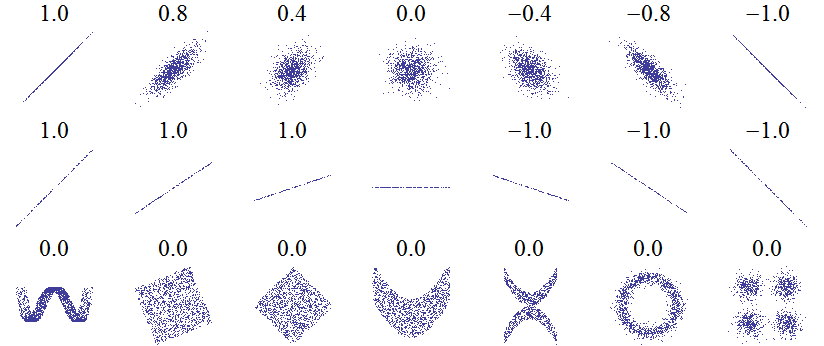
\includegraphics[height=2.5in]{figs/Correlation_examples.png}}
\caption{Examples of datasets with a range of correlations.}
\label{corr_examples}
\end{figure}

Figure~\ref{corr_examples} is from
\url{http://wikipedia.org/wiki/Correlation_and_dependence}.  It shows
scatterplots and correlation coefficients for several
carefully-constructed datasets.
\index{coefficient!correlation}
\index{scatter plot}
\index{plot!scatter}

The top row shows linear relationships with a range of correlations;
you can use this row to get a sense of what different values of
\myrho~look like.  The second row shows perfect correlations with a
range of slopes, which demonstrates that correlation is unrelated to
slope (we'll talk about estimating slope soon).  The third row shows
variables that are clearly related, but because the relationship is
non-linear, the correlation coefficient is 0.

The moral of this story is that you should always look at a scatterplot of
your data before blindly computing a correlation coefficient.
\index{correlation coefficient}
\index{coefficient!correlation}

\begin{exercise}
Write a function called {\tt Corr} that takes two lists and
computes their correlation.  Hint: use {\tt thinkstats.Var} and
the {\tt Cov} function you wrote in the previous exercise.
\index{variance}
\index{covariance}

To test your function, compute the covariance of a list with itself
and confirm that Corr(\X, \X) is 1.  You can download a solution
from \url{http://thinkstats.com/correlation.py}.
\index{{\tt correlation.py}}

\end{exercise}


\section{Making scatterplots in pyplot}
\index{scatter plot}
\index{plot!scatter}
\index{pyplot}

\begin{figure}
% brfss_corr.py
\centerline{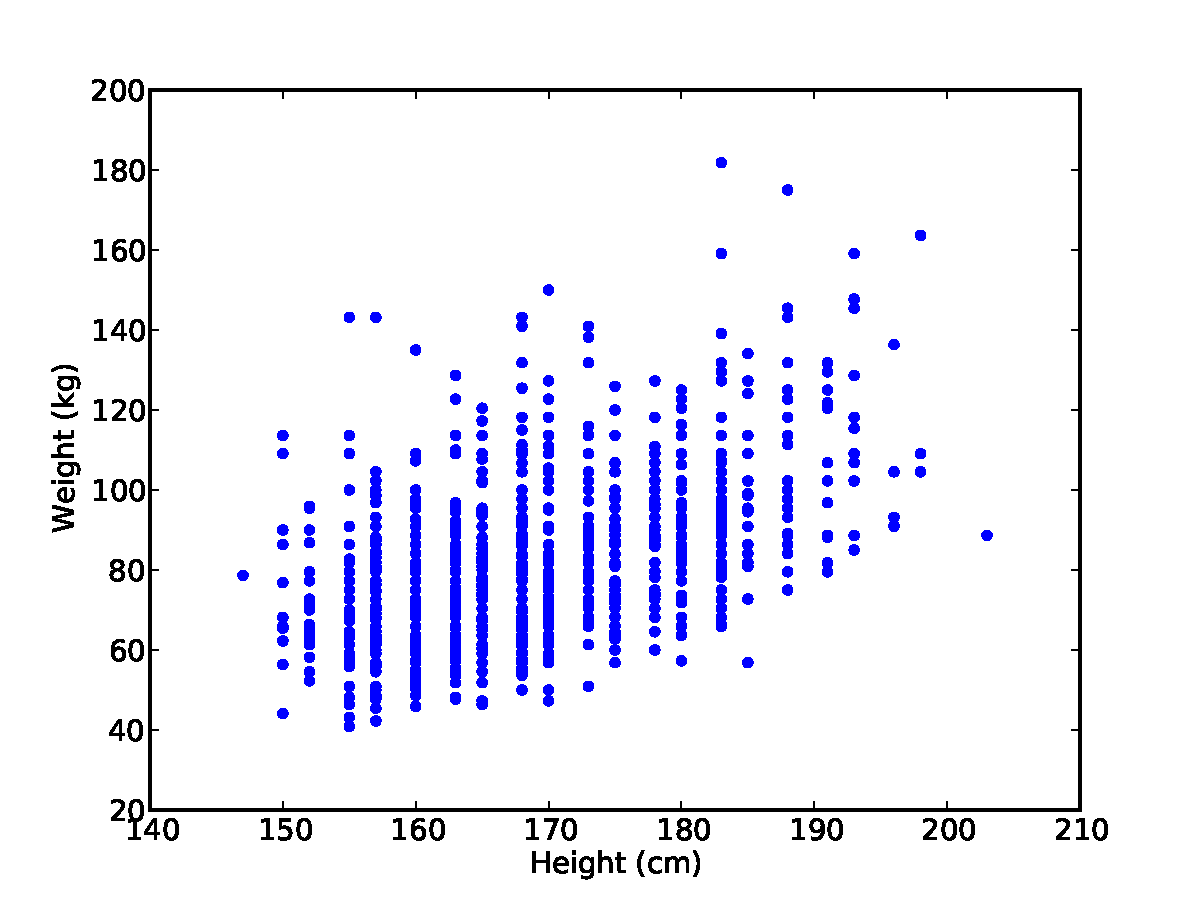
\includegraphics[height=2.5in]{figs/scatter1.pdf}}
\caption{Simple scatterplot of weight versus height for the respondents
in the BRFSS.}
\label{scatterplot1}
\end{figure}

\begin{figure}
% brfss_corr.py
\centerline{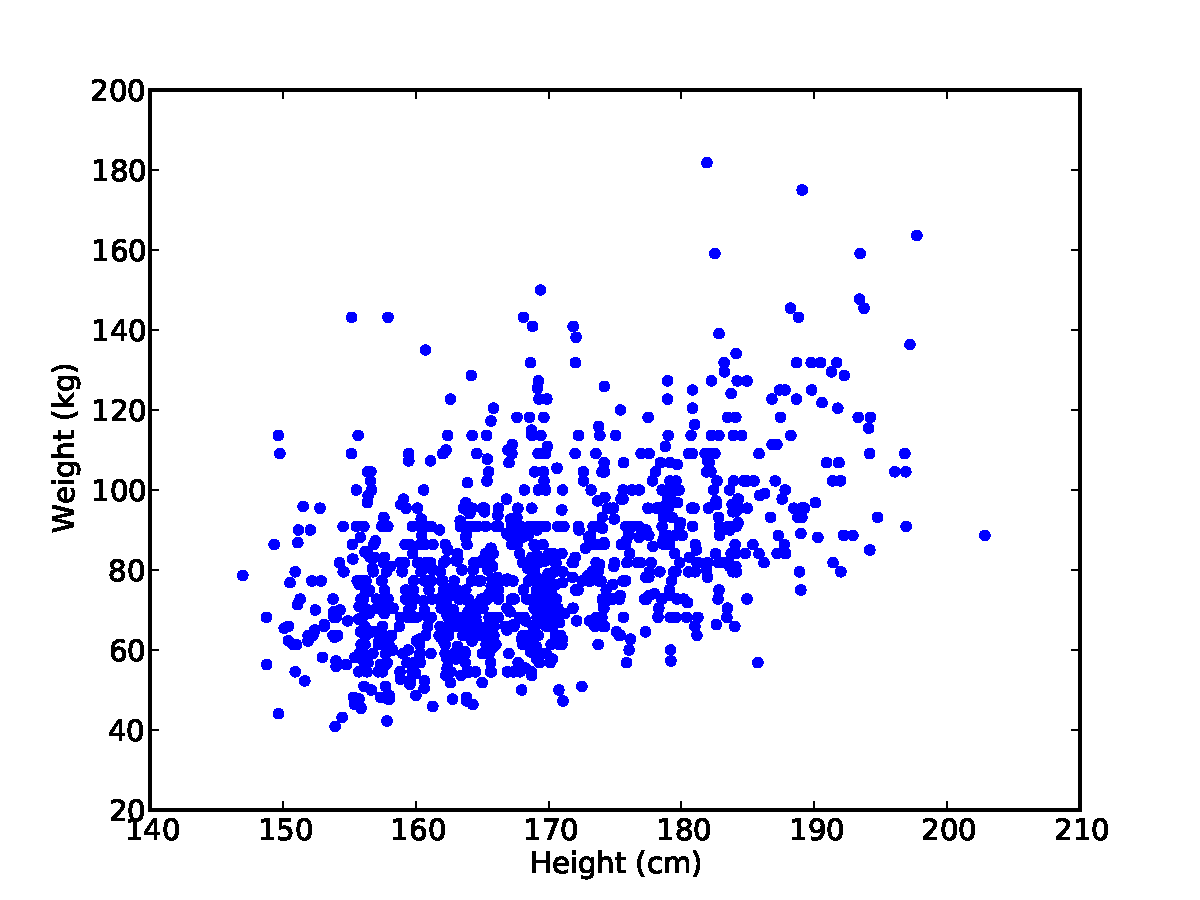
\includegraphics[height=2.5in]{figs/scatter2.pdf}}
\caption{Scatterplot with jittered data.}
\label{scatterplot2}
\end{figure}

\begin{figure}
% brfss_corr.py
\centerline{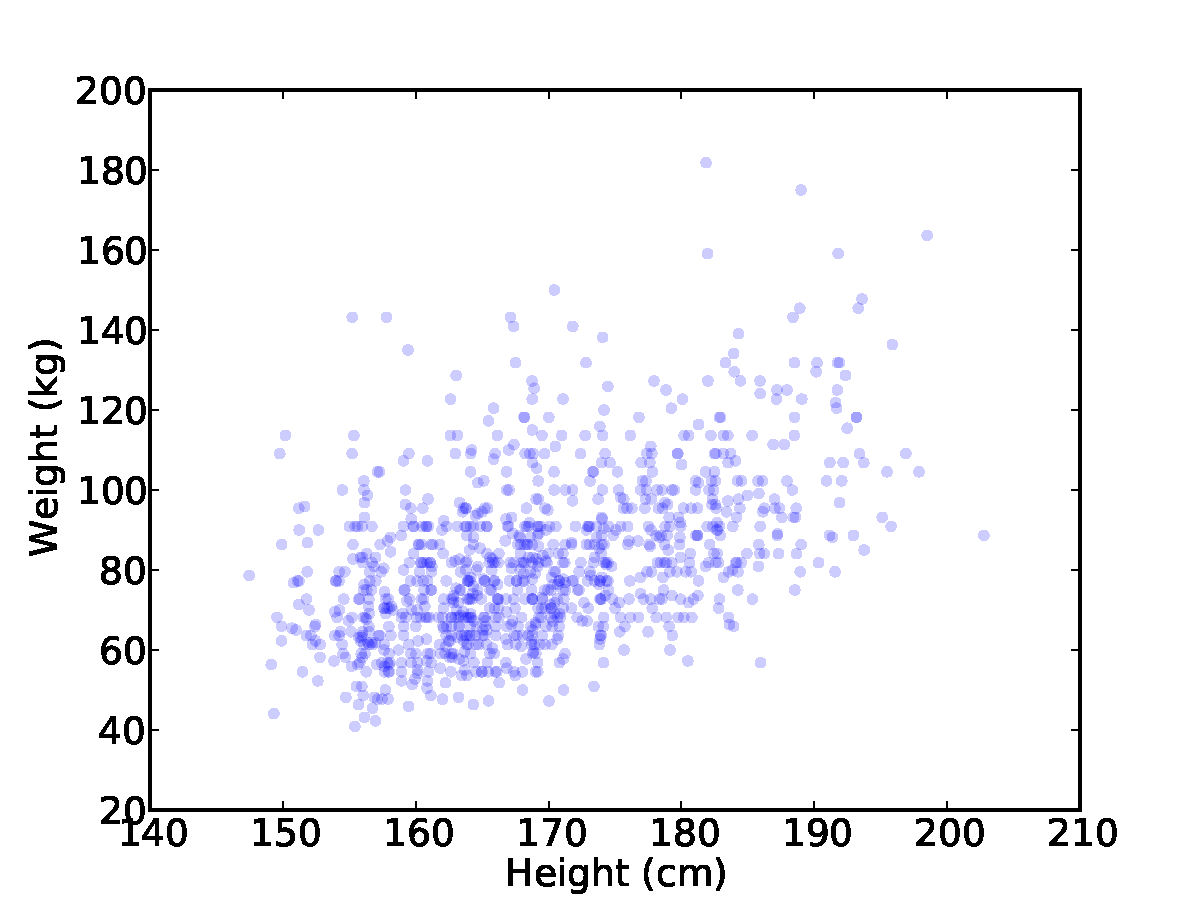
\includegraphics[height=2.5in]{figs/scatter3.pdf}}
\caption{Scatterplot with jittering and transparency.}
\label{scatterplot3}
\end{figure}

\begin{figure}
% brfss_corr.py
\centerline{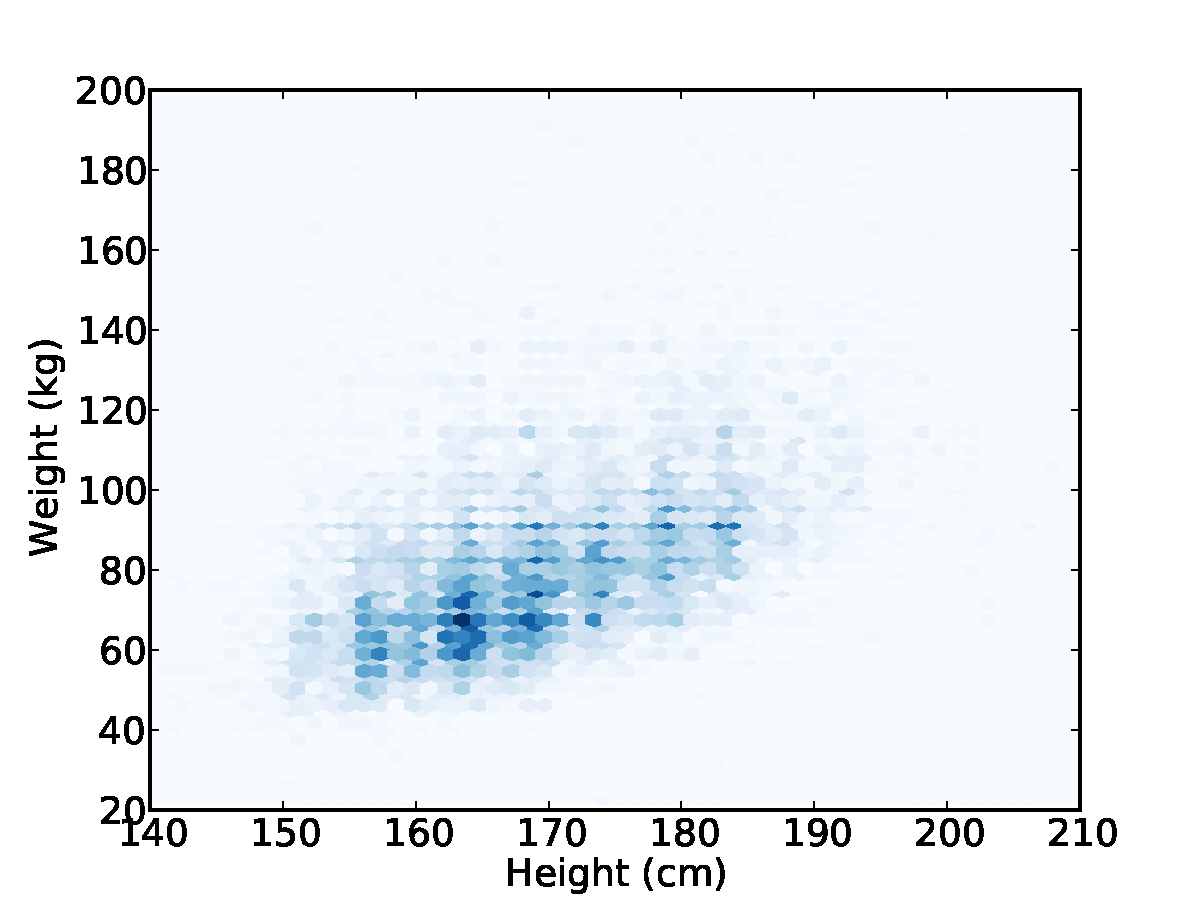
\includegraphics[height=2.5in]{figs/scatter4.pdf}}
\caption{Scatterplot with binned data using {\tt pyplot.hexbin}.}
\label{scatterplot4}
\end{figure}
\index{Behavioral Risk Factor Surveillance System}
\index{BRFSS}

The simplest way to check for a relationship between two variables
is a scatterplot, but making a good scatterplot is not always easy.
As an example, I'll plot weight versus height for the respondents
in the BRFSS (see Section~\ref{lognormal}).  {\tt pyplot} provides
a function named {\tt scatter} that makes scatterplots:
%
\begin{verbatim}
import matplotlib.pyplot as pyplot
pyplot.scatter(heights, weights)
\end{verbatim}

Figure~\ref{scatterplot1} shows the result.  Not surprisingly, it
looks like there is a positive correlation: taller people tend to be
heavier.  But this is not the best representation of the data, because
the data are packed into columns.  The problem is that the heights
were rounded to the nearest inch, converted to centimeters, and
then rounded again.  Some information is lost in translation.
\index{height}
\index{weight}
\index{jitter}

We can't get that information back, but we can minimize the effect on
the scatterplot by {\bf jittering} the data, which means adding random
noise to reverse the effect of rounding off.  Since these measurements
were rounded to the nearest inch, they can be off by up to 0.5 inches or
1.3 cm.  So I added uniform noise in the range \minus1.3 to 1.3:
\index{uniform distribution}
\index{distribution!uniform}
\index{noise}
%
\begin{verbatim}
jitter = 1.3
heights = [h + random.uniform(-jitter, jitter) for h in heights]
\end{verbatim}

Figure~\ref{scatterplot2} shows the result.  Jittering the data makes
the shape of the relationship clearer.  In general you should only jitter
data for purposes of visualization and avoid using jittered data
for analysis.

Even with jittering, this is not the best way to represent the data.
There are many overlapping points, which hides data
in the dense parts of the figure and gives disproportionate emphasis
to outliers.
\index{outlier}

We can solve that with the {\tt alpha} parameter, which makes
the points partly transparent:
%
\begin{verbatim}
pyplot.scatter(heights, weights, alpha=0.2)
\end{verbatim}
%
Figure~\ref{scatterplot3} shows the result.  Overlapping data
points look darker, so darkness is proportional to density.  In this
version of the plot we can see an apparent artifact: a horizontal line
near 90 kg or 200 pounds.  Since this data is based on self-reports in
pounds, the most likely explanation is some responses were rounded off
(possibly down).

Using transparency works well for moderate-sized datasets, but this
figure only shows the first 1000 records in the BRFSS, out of a total
of 414509.
\index{hexbin plot}
\index{plot!hexbin}

To handle larger datasets, one option is a hexbin plot, which divides
the graph into hexagonal bins and colors each bin according to how many
data points fall in it.  {\tt pyplot} provides a function called 
{\tt hexbin}:
%
\begin{verbatim}
pyplot.hexbin(heights, weights, cmap=matplotlib.cm.Blues)
\end{verbatim}
%
Figure~\ref{scatterplot4} shows the result with a blue colormap.
An advantage of a hexbin is that it shows the shape of the relationship
well, and it is efficient for large datasets.  A drawback is that
it makes the outliers invisible.
\index{colormap}
\index{grayscale}

The moral of this story is that it is
not easy to make a scatterplot that is not potentially misleading.
You can download the code for these figures from
\url{http://thinkstats.com/brfss_scatter.py}.
\index{{\tt brfss\_scatter.py}}

\section{Spearman's rank correlation}

Pearson's correlation works well if the relationship between variables
is linear and if the variables are roughly normal.  But it is not
robust in the presence of outliers.
\index{Pearson coefficient of correlation}
\index{Spearman coefficient of correlation}
\index{coefficient!correlation}
\index{normal distribution}
\index{distribution!normal}
\index{Gaussian distribution}
\index{distribution!Gaussian}

Anscombe's quartet demonstrates this effect; it contains four data
sets with the same correlation.  One is a linear relation with random
noise, one is a non-linear relation, one is a perfect relation with an
outlier, and one has no relation except an artifact caused by an
outlier.  You can read more about it at
\url{http://wikipedia.org/wiki/Anscombe's_quartet}.
\index{Anscombe's quartet}

Spearman's rank correlation is an alternative that mitigates the
effect of outliers and skewed distributions.  To compute Spearman's
correction, we have to compute the {\bf rank} of each value, which is its
index in the sorted sample.  For example, in the sample \{7, 1, 2, 5\}
the rank of the value 5 is 3, because it appears third if we sort
the elements.  Then we compute Pearson's correlation for the ranks.

An alternative to Spearman's is to apply a transform that makes the
data more nearly normal, the compute Pearson's correlation for the
transformed data.  For example, if the data are approximately
lognormal, you could take the log of each value and compute the
correlation of the logs.
\index{lognormal distribution}
\index{distribution!lognormal}

\begin{exercise}
Write a function that takes a sequence and returns a list that
contains the rank for each element.  For example, if the sequence is
\{7, 1, 2, 5\}, the result should be \{ 4, 1, 2, 3\}.

If the same value appears more than once, the strictly correct
solution is to assign each of them the average of their ranks.  But if
you ignore that and assign them ranks in arbitrary order, the error is
usually small.

Write a function that takes two sequences (with the same length) and
computes their Spearman rank coefficient.  You can download a solution
from \url{http://thinkstats.com/correlation.py}.
\index{{\tt correlation.py}}
\index{Spearman coefficient of correlation}
\index{coefficient!correlation}

\end{exercise}


\begin{exercise}
Download \url{http://thinkstats.com/brfss.py} and
\url{http://thinkstats.com/brfss_scatter.py}.  Run them and confirm that you
can read the BFRSS data and generate scatterplots.
\index{Behavioral Risk Factor Surveillance System}
\index{BRFSS}
\index{{\tt brfss.py}}
\index{{\tt brfss\_scatter.py}}

Comparing the scatterplots to Figure~\ref{corr_examples}, what value
do you expect for Pearson's correlation?  What value do you get?
\index{weight!adult}
\index{adult weight}
\index{lognormal distribution}
\index{distribution!lognormal}
\index{outlier}

Because the distribution of adult weight is lognormal, there are
outliers that affect the correlation.  Try plotting
log(weight) versus height, and compute Pearson's
correlation for the transformed variable.

Finally, compute Spearman's rank correlation for weight and height.
Which coefficient do you think is the best measure of the strength of
the relationship?  You can download a solution from
\url{http://thinkstats.com/brfss_corr.py}.
\index{{\tt brfss\_corr.py}}

\end{exercise}


\section{Least squares fit}

Correlation coefficients measure the strength and sign of a
relationship, but not the slope.  There are several ways to estimate
the slope; the most common is a {\bf linear least squares fit}.  A
``linear fit'' is a line intended to model the relationship between
variables.  A ``least squares'' fit is one that minimizes the mean
squared error (MSE) between the line and the data\footnote{See
  \url{http://wikipedia.org/wiki/Simple_linear_regression}.}.
\index{least squares fit}
\index{linear least squares}
\index{coefficient!correlation}
\index{linear regression}

Suppose we have a sequence of points, \Y, that we want to express as a
function of another sequence \X.  If there is a linear relationship
between \X~and \Y~with intercept \myinter~and slope \myslope, we
expect each \y\sub{i} to be roughly \myinter~+ \myslope~\x\sub{i}.
\index{residual}

But unless the correlation is perfect, this prediction is only
approximate.  The deviation, or {\bf residual}, is 

\Eqn{ \myeps\sub{i}~=~(\myinter~+~\myslope \x\sub{i})~\minus~\y\sub{i} }

The residual might be due to random factors like measurement error,
or non-random factors that are unknown.  For example, if we are
trying to predict weight as a function of height, unknown factors
might include diet, exercise, and body type.
\index{slope}
\index{intercept}

If we get the parameters \myinter~and \myslope~wrong, the residuals
get bigger, so it makes intuitive sense that the parameters we want
are the ones that minimize the residuals.

As usual, we could minimize the absolute value of the
residuals, or their squares, or their cubes, etc.  The most common
choice is to minimize the sum of squared residuals
%
\[ \min_{\inter, \slope} \sum \eps_i^2 \]
%
Why?  There are three good reasons and one bad one:

\begin{itemize}

\item Squaring has the obvious feature of treating positive and
negative residuals the same, which is usually what we want.

\item Squaring gives more weight to large residuals, but not
so much weight that the largest residual always dominates.

\item If the residuals are independent of \x, random, and normally
  distributed with \mymu~=~0 and constant (but unknown) \mysigma, then
  the least squares fit is also the maximum likelihood estimator of
  \myinter~and \myslope.\footnote{See Press et al., {\em Numerical Recipes in C},
    Chapter 15 at \url{http://www.nrbook.com/a/bookcpdf/c15-1.pdf}.}
\index{MLE}
\index{maximum likelihood estimator}

\item The values of $\hat{\inter}$ and $\hat{\slope}$ that minimize
  the squared residuals can be computed efficiently.

\end{itemize}

That last reason made sense when computational efficiency was more
important than choosing the method most appropriate to the problem
at hand.  That's no longer the case, so it is worth considering
whether squared residuals are the right thing to minimize.
\index{computation}

For example, if you are using values of \X~to predict values of \Y,
guessing too high might be better (or worse) than guessing too low.
In that case you might want to compute some cost function,
cost(\myeps\sub{i}), and minimize total cost.
\index{cost function}

However, computing a least squares fit is quick, easy and often good
enough, so here's how:

\begin{enumerate}

\item Compute the sample means, \myxbar~and \myybar, the variance
of \X, and the covariance of \X~and \Y.

\item The estimated slope is
%
\[ \hat{\slope} = \frac{Cov(X,Y)}{Var(X)} \]
%
\item And the intercept is
%
\[ \hat{\inter} = \ybar - \hat{\slope} \xbar \]
%
\end{enumerate}

To see how this is derived, you can read
\url{http://wikipedia.org/wiki/Numerical_methods_for_linear_least_squares}.


\begin{exercise}
Write a function named {\tt LeastSquares} that takes \X~and \Y~and
computes $\hat{\inter}$ and $\hat{\slope}$.  You can download a
solution from \url{http://thinkstats.com/correlation.py}.  \index{{\tt
    correlation.py}}

\end{exercise}

\begin{exercise}
Using the data from the BRFSS again, compute the linear least squares
fit for log(weight) versus height.  You can download a
solution from \url{http://thinkstats.com/brfss_corr.py}.
\index{Behavioral Risk Factor Surveillance System}
\index{BRFSS}
\index{{\tt brfss\_corr.py}}

\end{exercise}


\begin{exercise}
The distribution of wind speeds in a given location determines the
wind power density, which is an upper bound on the average power that
a wind turbine at that location can generate.  According to some
sources, empirical distributions of wind speed are well modeled by a
Weibull distribution (see
\url{http://wikipedia.org/wiki/Wind_power#Distribution_of_wind_speed}).
\index{wind speed}
\index{wind power density}
\index{turbine}
\index{Weibull distribution}
\index{distribution!Weibull}

To evaluate whether a location is a viable site for a wind turbine,
you can set up an anemometer to measure wind speed for a period of
time.  But it is hard to measure the tail of the wind speed distribution
accurately because, by definition, events in the tail don't happen
very often.
\index{tail}

One way to address this problem is to use measurements to estimate the
parameters of a Weibull distribution, then integrate over the
continuous PDF to compute wind power density.
\index{PDF}

To estimate the parameters of a Weibull distribution, we can use the
transformation from Exercise~\ref{weibull} and then use a linear fit
to find the slope and intercept of the transformed data.

Write a function that takes a sample from a Weibull distribution and
estimates its parameters.

Now write a function that takes the parameters of a Weibull distribution
of wind speed and computes average wind power density (you might have
to do some research for this part).

\end{exercise}


\section{Goodness of fit}
\index{goodness of fit}
\index{fit, goodness}

Having fit a linear model to the data, we might want to know how good
it is.  Well, that depends on what it's for.  One way to evaluate a
model is its predictive power.

In the context of prediction, the quantity we are trying to guess is
called a {\bf dependent variable} and the quantity we are using to
make the guess is called an {\bf explanatory} or {\bf independent
  variable}.
\index{dependent variable}
\index{explanatory variable}
\index{independent variable}
\index{coefficient!determination}

To measure the predictive power of a model, we can compute the {\bf
  coefficient of determination}, more commonly known as ``R-squared'':
%
\[ R^2 = 1 - \frac{Var(\eps)}{Var(Y)}\]
%
To understand what \R\super{2} means, suppose (again) that you are trying
to guess someone's weight.  If you didn't know anything about them,
your best strategy would be to guess \myybar; in
that case the MSE of your guesses would be Var(\Y):
%
\[ MSE = \frac{1}{n} \sum (\ybar - y_i)^2 = Var(Y) \]
%
But if I told you their height, you would guess $\hat{\inter} +
\hat{\slope}$ \x\sub{i}; in that case your MSE would be Var(\myeps).
%
\[ MSE = 
\frac{1}{n} \sum (\hat{\inter} + \hat{\slope} x_i - y_i)^2 =
Var(\eps) \]
%
So the term Var(\myeps)/Var(\Y) is the ratio of mean squared error with
and without the explanatory variable, which is the fraction of
variability left unexplained by the model.  The complement, \R\super{2},
is the fraction of variability explained by the model.
\index{variability}

If a model yields \R\super{2}~=~0.64, you could say that the model explains
64\% of the variability, or it might be more precise to say that it
reduces the MSE of your predictions by 64\%.

In the context of a linear least squares model, it turns out that
there is a simple relationship between the coefficient of
determination and Pearson's correlation coefficient, \myrho:

\Eqn{ \R\super{2} = \myrho\super{2} }

See \url{http://wikipedia.org/wiki/Howzzat}!
\index{howzzat}

\begin{exercise}
The Wechsler Adult Intelligence Scale (WAIS) is meant to be a measure
of intelligence; scores are calibrated so that the mean and standard
deviation in the general population are 100 and 15.
\index{Adult Intelligence Scale}
\index{WAIS}
\index{IQ}
\index{intelligence}

Suppose that you wanted to predict someone's WAIS score based on their
SAT scores.  According to one study, there is a Pearson correlation of
0.72 between total SAT scores and WAIS scores.

If you applied your predictor to a large sample, what would you expect to
be the mean squared error (MSE) of your predictions?

Hint: What is the MSE if you always guess 100?
\end{exercise}


\begin{exercise}
Write a function named {\tt Residuals} that takes \X, \Y, $\hat{\inter}$
and $\hat{\slope}$ and returns a list of \myeps\sub{i}.
\index{residual}

Write a function named {\tt CoefDetermination} that takes the 
\myeps\sub{i}~and \Y~and returns \R\super{2}.  To test your functions, 
confirm that {\R\super{2}~=~\myrho\super{2}}.  You can download a solution
from \url{http://thinkstats.com/correlation.py}.
\index{{\tt correlation.py}}

\end{exercise}

\begin{exercise}
Using the height and weight data from the BRFSS (one more time),
compute $\hat{\inter}$, $\hat{\slope}$ and \R\super{2}.  If you were trying to guess
someone's weight, how much would it help to know their height?
You can download a solution from
\url{http://thinkstats.com/brfss_corr.py}.
\index{Behavioral Risk Factor Surveillance System}
\index{BRFSS}
\index{{\tt brfss\_corr.py}}

\end{exercise}


\section{Correlation and Causation}
\index{correlation}
\index{causation}
\index{xkcd}
\index{comic}
\index{Munroe, Randall}

The web comic {\tt xkcd} demonstrates the difficulty of inferring
causation:

\begin{figure}
\centerline{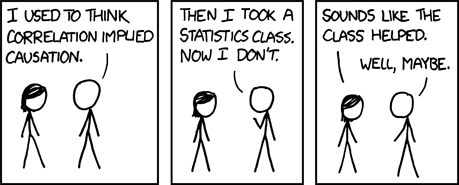
\includegraphics[width=4.0in]{figs/correlation.png}}
\caption{From {\tt xkcd.com} by Randall Munroe.}
\end{figure}

In general, a relationship between two variables does not tell you
whether one causes the other, or the other way around, or both, or
whether they might both be caused by something else altogether.

This rule can be summarized with the phrase ``Correlation
does not imply causation,'' which is so pithy it has its own
Wikipedia page: \url{http://wikipedia.org/wiki/Correlation_does_not_imply_causation}.

So what can you do to provide evidence of causation?

\begin{enumerate}

\item Use time.  If A comes before B, then A can cause B but not the
  other way around (at least according to our common understanding of
  causation).  The order of events can help us infer the direction
  of causation, but it does not preclude the possibility that something
  else causes both A and B.

\item Use randomness.  If you divide a large population into two
  groups at random and compute the means of almost any variable, you
  expect the difference to be small.  This is a consequence of the
  Central Limit Theorem (so it is subject to the same requirements).

  If the groups are nearly identical in all variable but one, you
  can eliminate spurious relationships.
\index{spurious relationship}

  This works even if you don't know what the relevant variables
  are, but it works even better if you do, because you can check that
  the groups are identical.

\end{enumerate}

These ideas are the motivation for the {\bf randomized controlled
trial}, in which subjects are assigned randomly to two (or more)
groups: a {\bf treatment} group that receives some kind of intervention,
like a new medicine, and a {\bf control group} that receives
no intervention, or another treatment whose effects are known.
\index{randomized controlled trial}
\index{controlled trial}
\index{treatment group}
\index{control group}
\index{medicine}

A randomized controlled trial is the most reliable way to demonstrate
a causal relationship, and the foundation of science-based medicine
(see \url{http://wikipedia.org/wiki/Randomized_controlled_trial}).

Unfortunately, controlled trials are only possible in the laboratory
sciences, medicine, and a few other disciplines.  In the social sciences,
controlled experiments are rare, usually because they are impossible
or unethical.

One alternative is to look for a {\bf natural experiment}, where
different ``treatments'' are applied to groups that are otherwise
similar.  One danger of natural experiments is that the groups might
differ in ways that are not apparent.  You can read more about this
topic at \url{http://wikipedia.org/wiki/Natural_experiment}.
\index{natural experiment}

In some cases it is possible to infer causal relationships using {\bf
  regression analysis}.  A linear least squares fit
is a simple form of regression that explains a dependent
variable using one explanatory variable.  There are similar
techniques that work with arbitrary numbers of independent variables.
\index{regression analysis}

I won't cover those techniques here, but there are also simple ways to
control for spurious relationships.  For example, in the NSFG, we saw
that first babies tend to be lighter than others (see
Section~\ref{birth_weights}).  But birth weight is also correlated
with the mother's age, and mothers of first babies tend to be younger
than mothers of other babies.
\index{birth weight}
\index{weight!birth}
\index{National Survey of Family Growth}
\index{NSFG}

So it may be that first babies are lighter because their mothers are
younger.  To control for the effect of age, we could divide the mothers
into age groups and compare birth weights for first babies and others
in each age group.
\index{pooled data}

If the difference between first babies and others is the same in
each age group as it was in the pooled data, we conclude
that the difference is not related to age.  If there is no difference,
we conclude that the effect is entirely due to age.  Or,
if the difference is smaller, we can quantify how much of the effect
is due to age.

\begin{exercise}
The NSFG data includes a variable named {\tt agepreg} that records
the age of the mother at the time of birth.
Make a scatterplot of mother's age and baby's weight for each live
birth.  Can you see a relationship?

Compute a linear least-squares fit for these variables.  What are the
units of the estimated parameters $\hat{\inter}$ and $\hat{\slope}$?
How would you summarize these results in a sentence or two?

Compute the average age for mothers of first babies and the average
age of other mothers.  Based on the difference in ages between the
groups, how much difference do you expect in the mean birth weights?
What fraction of the actual difference in birth weights is explained
by the difference in ages?

You can download a solution to this problem from
\url{http://thinkstats.com/agemodel.py}.  If you are curious about
multivariate regression, you can run \url{http://thinkstats.com/age_lm.py}
which shows how to use the R statistical computing package from
Python.  But that's a whole other book.
\index{{\tt agemodel.py}}
\index{{\tt age\_lm.py}}

\end{exercise}


\section{Glossary}

\begin{description}

\item[correlation:] a description of the dependence between variables.
\index{correlation}

\item[normalize:] To transform a set of values so that their mean is 0 and
their variance is 1.
\index{normalize}

\item[standard score:] A value that has been normalized.
\index{standard score}

\item[covariance:] a measure of the tendency of two variables
to vary together.
\index{covariance}

\item[rank:] The index where an element appears in a sorted list.
\index{rank}

\item[least squares fit:] A model of a dataset that minimizes the
sum of squares of the residuals.
\index{least squares fit}

\item[residual:] A measure of the deviation of an actual value from a model.
\index{residual}

\item[dependent variable:] A variable we are trying to predict or explain.
\index{dependent variable}

\item[independent variable:] A variable we are using to predict a dependent
variable, also called an explanatory variable.
\index{independent variable}

\item[coefficient of determination:] A measure of the goodness of fit
of a linear model.
\index{coefficient!determination}

\item[randomized controlled trial:] An experimental design in which subject
are divided into groups at random, and different groups are given different
treatments.
\index{randomized controlled trial}

\item[treatment:] An change or intervention applied to one group in a
controlled trial.
\index{treatment group}

\item[control group:] A group in a controlled trial that receives no
treatment, or a treatment whose effect is known.
\index{control group}

\item[natural experiment:] An experimental design that takes advantage of
a natural division of subjects into groups in ways that are at least
approximately random.
\index{natural experiment}

\end{description}


\printindex

\clearemptydoublepage
%\blankpage
%\blankpage
%\blankpage


\end{document}

%Chapter 10: time series

%serial correlation

%auto-correlation function

%generating random series with correlation

%violating the CLT and see if the sum of correlated normals is lognormal

%If so, maybe that explains adult weight distribution.




% Topics to consider in the future:

% Time series

% Correlation of adjacent elements

% Autocorrelation function

% Information theory: Paul Revere example

% Gelman's paradox
% \url{http://www.iq.harvard.edu/blog/sss/archives/2008/04/gelmans_paradox.shtml}

% regression to the mean experiment

% Poisson distribution

% example using csvDictReader


